\section{Photoproduction with linearly polarized beam}%
\label{sec:photoprod}

\subsection{Moment decomposition}%
\label{sec:photoprod:moment}

Systems of two distinguishable spinless particles can also be produced
in photo-production reactions using stationary proton targets.  As in
the case of diffractive reactions discussed in \cref{sec:diffraction},
we are interested in the intermediate meson resonances~$X$ that are
produced in these reactions and that decay into the observed
two-(pseudo)scalar system.  A typical example for such a process is
the reaction
\begin{equation}
  \label{eq:etaOrPr_pi_photoprod}
  \gamma\, p \to X^0\, p \to \etaOrPr\pi^0\, p,
\end{equation}
which is shown in \cref{fig:photoprod_etaprimepi}.  How to analyze
these reactions was studied in detail by the JPAC collaboration
in~\refsCite{Mathieu:2019fts,Mathieu:2019gxo}.  We will follow these
references here and will derive some equations.

\begin{figure}[bp]
  \centering%
  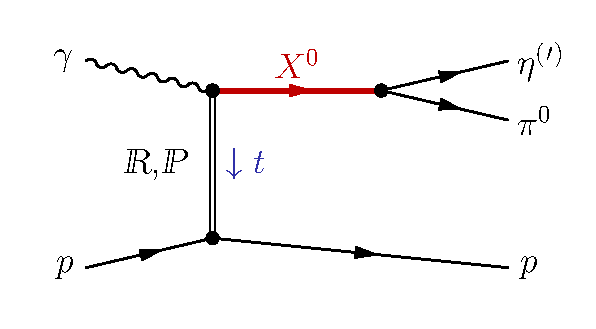
\includegraphics[width=0.5\textwidth]{photoproduction_x_etaprimepi_p}%
  \caption{Scattering of a real photon off a target proton mediated by
  Reggeon exchange.  In this photoproduction process, an intermediate
  state~$X^0$ with well-defined quantum numbers is produced, which in
  the example given here decays into the \etaOrPrPim channel.
  (\Confer~\cref{fig:diffraction_etaprimepi}.)}%
  \label{fig:photoprod_etaprimepi}%
\end{figure}

The analysis is based on the measured intensity distribution, \ie the
number density distribution of events, which is decomposed into
partial-wave amplitudes analogous to the diffractive case in
\cref{eq:diffraction_intensity}:\footnote{\label{fn:photoprod_ampl_redef}This
corresponds to Eq.~(A3) in \refCite{Mathieu:2019fts} with the
phase-space factor~$\kappa$ absorbed into the partial-wave amplitudes,
\ie with the redefinition $\prodAmp \to \prodAmp / \sqrt{\kappa}$ (see
also footnote~6 in \refCite{Mathieu:2019fts}), and with Eq.~(A5)
inserted.}\todo{Can we express this as $\abs{\text{amplitude}}^2$?}
\begin{equation}
  \label{eq:photoprod_intensity}
  \intensity(\Omega, \Phi; w, t)
  = \frac{\dif{N}}{\dif{w}\, \dif{t}\, \dif{\Omega}\, \dif{\Phi}}
  = \sum_{\substack{\ell m \\ \ell' m'}}^\infty
  Y_\ell^m(\Omega)~
  \dUnderbrace{\sum_{\substack{\lambda, \lambda' = \pm 1 \\ \mathclap{\lambda_1, \lambda_2 = \pm 1/2}}}
  \prodAmp^\ell_{\!m\, \lambda; \lambda_1\, \lambda_2}(w, t)\,
  \varrho^\gamma_{\lambda\, \lambda'}(\Phi)\,
  \prodAmp^{\ell' *}_{\!m'\, \lambda'; \lambda_1\, \lambda_2}(w, t)}{\equiv \varrho^{\ell\, \ell'}_{m\, m'}(w, t, \Phi)}~
  Y_{\ell'}^{m' *}(\Omega).
\end{equation}
Here, $N$~is the (acceptance-corrected) number of measured events,
$w$~is the invariant mass of the two-(pseudo)scalar system, $t$~is the
squared four-momentum transferred from the beam to the target
particle, $\Omega = (\theta, \phi)$ is the direction of one of the two
(pseudo)scalar mesons the~$X$ decays into, measured in the
Gottfried-Jackson or helicity rest frame of~$X$, and~$\Phi$ is the
azimuthal angle between the polarization vector of the linearly
polarized photon and the reaction plane in the $X$~rest frame.  The
$\prodAmp^\ell_{\!m\, \lambda; \lambda_1\, \lambda_2}(w, t)$ are
the partial-wave amplitudes that correspond to an intermediate state
with a spin, which is given by the relative orbital angular
momentum~$\ell$ between the two-(pseudo)scalar mesons, and a spin
projection~$m$ \wrt the chosen quantization axis (Gottfried-Jackson
frame: beam direction; helicity frame: momentum direction of~$X$).
This intermediate state is produced in the interaction of a photon
with helicity~$\lambda = \pm 1$ and a target proton with
helicity~$\lambda_1 = \pm 1/2$; the recoil proton has
helicity~$\lambda_2 = \pm 1/2$.  The angular distribution of the
$X$~decay products is given by the spherical harmonics
$Y_\ell^m(\Omega)$~\cite{wikipedia:sphericalHarm} and the dependence
on the polarization angle~$\Phi$ is given by the photon spin-density
matrix~$\mat{\upvarrho}^\gamma(\Phi)$.  In
\cref{eq:photoprod_intensity}, $\varrho^{\ell\, \ell'}_{m\, m'}(w, t,
\Phi)$ is the spin-density matrix element of~$X$ defined analogously
to the diffractive case in \cref{eq:diffraction_spin_dens_def}.

Using the fact that the three Pauli matrices $\vec{\mat{\upsigma}} =
(\mat{\upsigma}_1, \mat{\upsigma}_2, \mat{\upsigma}_3)^T$ and
$\mat{I}_{2 \times 2}$ form a complete set in the space of Hermitian
$2 \times 2$ matrices, we can expand $\mat{\upvarrho}^\gamma(\Phi)$,
\ie
\begin{equation}
  \mat{\upvarrho}^\gamma(\Phi)
  = \frac{1}{2}\, \mat{I}_{2 \times 2} + \frac{1}{2}\, \vec{P}_\gamma(\Phi) \cdot \vec{\mat{\upsigma}}.
\end{equation}
Here, the vector $\vec{P}_\gamma(\Phi)$ describes the photon
polarization.  Its length~$0 \leq P_\gamma \leq 1$ is the degree of
polarization and its direction depends on the kind of
polarization:\footnote{See Eq.~(19) in \refCite{Schilling:1969um}.}
\begin{equation}
  \vec{P}_\gamma(\Phi)
  = \begin{cases*}
    P_\gamma\, (0, 0, \lambda)^T                & for circularly polarized photons with $\lambda = \pm 1$, \\
    -P_\gamma\, (\cos(2 \Phi), \sin(2 \Phi), 0)^T & for linearly polarized photons with polarization angle~$\Phi$.
  \end{cases*}
\end{equation}
Hence, for linearly polarized photons, the intensity distribution in
\cref{eq:photoprod_intensity} can be written as the sum of three
terms:\footnote{See Eq.~(B4) in \refCite{Mathieu:2019fts}.}
\begin{equation}
  \label{eq:photoprod_intensity_sum}
  \intensity(\Omega, \Phi; w, t)
  = \intensity_0(\Omega; w, t)
  - \intensity_1(\Omega; w, t)\, P_\gamma\, \cos(2 \Phi)
  - \intensity_2(\Omega; w, t)\, P_\gamma\, \sin(2 \Phi)
\end{equation}
with the intensity components
\begin{equation}
  \label{eq:photoprod_intensity_components}
  \intensity_i(\Omega; w, t)
  = \sum_{\substack{\ell m \\ \ell' m'}}^\infty
  Y_\ell^m(\Omega)\,
  \prescript{i}{}{\varrho}^{\ell\, \ell'}_{m\, m'}(w, t)\,
  Y_{\ell'}^{m' *}(\Omega);
  \quad i = 0, 1, 2
\end{equation}
and the spin-density matrix components\footnote{See Eq.~(11) in
\refCite{Mathieu:2019fts}.}
\begin{align}
  \label{eq:photoprod_rho_0}
  \prescript{0}{}{\varrho}^{\ell\, \ell'}_{m\, m'}(w, t)
  ={}& \frac{1}{2}\quad \sum_{\substack{\lambda = \pm 1 \\ \mathclap{\lambda_1, \lambda_2 = \pm 1/2}}}
  \prodAmp^\ell_{\!m\, \lambda; \lambda_1\, \lambda_2}(w, t)\,
  \prodAmp^{\ell' *}_{\!m'\, \lambda; \lambda_1\, \lambda_2}(w, t)
  \\
  \label{eq:photoprod_rho_1}
  \prescript{1}{}{\varrho}^{\ell\, \ell'}_{m\, m'}(w, t)
  ={}& \frac{1}{2}\quad \sum_{\substack{\lambda = \pm 1 \\ \mathclap{\lambda_1, \lambda_2 = \pm 1/2}}}
  \prodAmp^\ell_{\!m\, {-\lambda}; \lambda_1\, \lambda_2}(w, t)\,
  \prodAmp^{\ell' *}_{\!m'\, \lambda; \lambda_1\, \lambda_2}(w, t)
  \\
  \label{eq:photoprod_rho_2}
  \prescript{2}{}{\varrho}^{\ell\, \ell'}_{m\, m'}(w, t)
  ={}& \frac{\imag}{2}\quad \sum_{\substack{\lambda = \pm 1 \\ \mathclap{\lambda_1, \lambda_2 = \pm 1/2}}}
  \lambda\,
  \prodAmp^\ell_{\!m\, {-\lambda}; \lambda_1\, \lambda_2}(w, t)\,
  \prodAmp^{\ell' *}_{\!m'\, \lambda; \lambda_1\, \lambda_2}(w, t).
\end{align}
Using the above, the spin-density matrix elements of~$X$ in
\cref{eq:photoprod_intensity} are given by
\begin{equation}
  \label{eq:photoprod_spin_dens_sum}
  \varrho^{\ell\, \ell'}_{m\, m'}(w, t, \Phi)
  = \prescript{0}{}{\varrho}^{\ell\, \ell'}_{m\, m'}(w, t)
  - \prescript{1}{}{\varrho}^{\ell\, \ell'}_{m\, m'}(w, t)\, P_\gamma\, \cos(2 \Phi)
  - \prescript{2}{}{\varrho}^{\ell\, \ell'}_{m\, m'}(w, t)\, P_\gamma\, \sin(2 \Phi).
\end{equation}

Note that in \cref{eq:photoprod_intensity_sum}, the $\Phi$~dependence
is separated, \ie neither the $\intensity_i$ nor the
$\prescript{i}{}{\varrho}^{\ell\, \ell'}_{m\, m'}$ depend on~$\Phi$.
The three intensity components $\intensity_i(\Omega; w, t)$ (as well
as the three spin-density matrix components in
\cref{eq:photoprod_spin_dens_sum}) are modulated by different
$\Phi$~dependences.  From \cref{eq:photoprod_intensity_sum} follows
that
\begin{equation}
  \label{eq:photoprod_unpolarized_intensity}
  \int_{-\pi}^{+\pi}\hspace{-1.2em} \dif{\Phi}\, \intensity(\Omega, \Phi; w, t)
  = 2 \pi\, \intensity_0(\Omega; w, t).
\end{equation}
This means that $\mathcal{I}_0(\Omega; w, t)$ corresponds---up to a
factor of $2 \pi$---to the unpolarized intensity distribution and is
equivalent to the intensity for the diffractive case in
\cref{eq:diffraction_intensity}.  The other two components
$\intensity_{1, 2}(\Omega; w, t)$ represent additional information
that is accessible in photoproduction with linearly polarized beam.
They depend on the photon polarization and are hence modulated by
different $\Phi$~dependences.  Note that the functions
$\cBrk[1]{f_0(\Phi), f_1(\Phi), f_2(\Phi)} = \cBrk[1]{1, \cos(2 \Phi),
\sin(2 \Phi)}$ that modulate the intensity components constitute an
orthogonal set of functions, \ie
\begin{equation}
  \label{eq:photoprod_orthogonality_phi}
  \int_{-\pi}^{+\pi}\hspace{-1.2em} \dif{\Phi}\, f_i(\Phi)\, f_j(\Phi)
  = (1 + \delta_{i 0})\, \pi\, \delta_{i j};
  \quad i, j = 0 ,1, 2.
\end{equation}

Like for the diffractive case, the partial-wave analysis as well as
the moment decomposition are performed in narrow kinematic cells in
the $(w, t)$ plane, assuming that within each cell all quantities are
in good approximation independent of~$w$ and~$t$.  To simplify
notation we hence omit the~$w$ and $t$~dependencies in all formulas
below, \ie the given formulas are valid in a $(w, t)$ cell.

Analogously to the diffractive case in
\cref{eq:diffraction_intensity_moments}, we decompose the intensity in
\cref{eq:photoprod_intensity_sum} into spherical harmonics to obtain
the moments.  Due to the orthogonality of the $\intensity_i$ terms in
$\Phi$~space, we can decompose each intensity component
separately:\footnote{See Eq.~(A8) in \refCite{Mathieu:2019fts}.}
\begin{align}
  \label{eq:photoprod_intensity_moments_norm_unpol}
  \intensity_0(\Omega)
  ={}& \sum_{L M}^\infty \sqrt{\frac{2 L + 1}{4 \pi}}\, H_0(L, M)\, Y_L^M(\Omega)
  \\
  \label{eq:photoprod_intensity_moments_norm_pol}
  \intensity_{1, 2}(\Omega)
  ={}& -\sum_{L M}^\infty \sqrt{\frac{2 L + 1}{4 \pi}}\, H_{1, 2}(L, M)\, Y_L^M(\Omega).
\end{align}
Here, we have used the same normalization as in
\cref{sec:diffraction:moments_norm}.
\Cref{eq:photoprod_intensity_moments_norm_unpol} is equivalent to
\cref{eq:diffraction_intensity_moments_norm}.  The minus sign in
\cref{eq:photoprod_intensity_moments_norm_pol} is introduced in order
to compensate that the respective intensity components contribute
negatively to the intensity distribution in
\cref{eq:photoprod_intensity_sum}.\footnote{\label{fn:photoprod_intensity_sign}The
minus sign also ensures that $H_1(0, 0) \geq 0$ if the wave set
contains only positive-reflectivity waves with $m \geq 0$ (see
\cref{sec:photoprod:reflectivity}, in particular
\cref{eq:photoprod_H_1_0_0_refl_2}, and Appendix~D in
\refCite{Mathieu:2019fts}).}

The corresponding moments are
\begin{equation}
  \label{eq:photoprod_moments_norm}
  H_i(L, M)
  = \frac{1}{\pi}\, \sqrt{\frac{4 \pi}{2 L + 1}} \int_{4 \pi}\!\!\!\! \dif{\Omega} \int_{-\pi}^{+\pi}\hspace{-1.2em} \dif{\Phi}\,
  \intensity(\Omega, \Phi)\, Y_L^{M *}(\Omega) \times \begin{cases*}
    1 / 2                   & for $i = 0$, \\
    \cos(2 \Phi) / P_\gamma & for $i = 1$, \\
    \sin(2 \Phi) / P_\gamma & for $i = 2$.
  \end{cases*}
\end{equation}
Here, $H_0(L, M)$ is equivalent to \cref{eq:diffraction_moments_norm}
for the diffractive case.\footnote{The $1 / (2 \pi)$ factor comes from
\cref{eq:photoprod_unpolarized_intensity}.}  The two polarized moments
$H_{1, 2}(L, M)$ represent orthogonal angular distributions in~$\Phi$
(see \cref{eq:photoprod_orthogonality_phi}).


\subsection{Relation between moments and partial-wave amplitudes}%
\label{sec:photoprod:moments_pw}

As in the diffractive case (\confer\
\cref{eq:diffraction_moments_pw_norm}), the moments are linear
combinations of the elements of the respective components of the
spin-density matrix of~$X$.  We see this by inserting
\cref{eq:spherical_harm_prod} into
\cref{eq:photoprod_intensity_components} and comparing with
\cref{eq:photoprod_intensity_moments_norm_unpol,eq:photoprod_intensity_moments_norm_pol},
\ie\footnote{See Eq.~(A9) in \refCite{Mathieu:2019fts}.}
\begin{align}
  \label{eq:photoprod_moment_unpol_pw}
  H_0(L, M)
  ={}& \sum_{\substack{\ell m \\ \ell' m'}}^\infty \sqrt{\frac{2 \ell' + 1}{2 \ell + 1}}
  \clebsch{\ell'}{0}{L}{0}{\ell}{0}\, \clebsch{\ell'}{m'}{L}{M}{\ell}{m}\,
  \prescript{0}{}{\varrho}^{\ell\, \ell'}_{m\, m'}
  \\
  \label{eq:photoprod_moments_pol_pw}
  H_{1, 2}(L, M)
  ={}& -\sum_{\substack{\ell m \\ \ell' m'}}^\infty \sqrt{\frac{2 \ell' + 1}{2 \ell + 1}}
  \clebsch{\ell'}{0}{L}{0}{\ell}{0}\, \clebsch{\ell'}{m'}{L}{M}{\ell}{m}\,
  \prescript{1, 2}{}{\varrho}^{\ell\, \ell'}_{m\, m'},
\end{align}
where the $\prescript{i}{}{\varrho}^{\ell\, \ell'}_{m\, m'}$ are given
by \crefrange{eq:photoprod_rho_0}{eq:photoprod_rho_2}.  For given~$(L,
M)$, the Clebsch-Gordan coefficients restrict the sums to those
quantum-number combinations, for which $\ell' + L + \ell =
\text{even}$ (see \cref{eq:ang_mom_sum}), $\abs{\ell' - L} \leq \ell
\leq \ell' + L$, and $m = m' + M$.  This means that if the
partial-wave amplitudes vanish for $\ell, \ell' > \ell_\text{max}$ the
moments~$H_i(L, M)$ will vanish $L > 2 \ell_\text{max}$.


\subsection{Symmetry properties of moments}%
\label{sec:photo_prod:moments_sym}

To derive the symmetry relations for the photoproduction moments we
use the same approach as in \cref{sec:diffraction:moments_sym}.

From the symmetry property of the spherical harmonics in
\cref{eq:spherical_harm_sym} and the definition of the moments in
\cref{eq:photoprod_moments_norm}, we get
\begin{align}
  \label{eq:photoprod_moments_sym_1}
  H_i^*(L, M)
  ={}& (-1)^M\, \frac{1}{\pi}\, \sqrt{\frac{4 \pi}{2 L + 1}}
  \int_{4 \pi}\!\!\!\! \dif{\Omega} \int_{-\pi}^{+\pi}\hspace{-1.2em} \dif{\Phi}\,
  \intensity(\Omega, \Phi)\, Y_L^{(-M) *}(\Omega) \times \begin{cases*}
    1 / 2                   & for $i = 0$, \\
    \cos(2 \Phi) / P_\gamma & for $i = 1$, \\
    \sin(2 \Phi) / P_\gamma & for $i = 2$
  \end{cases*}
  \\
  ={}& (-1)^M\, H_i(L, {-M}),
\end{align}
which is analogous to \cref{eq:diffraction_moment_sym_1}.

Since the formulas for the intensity components in
\cref{eq:photoprod_intensity_moments_norm_unpol,eq:photoprod_intensity_moments_norm_pol}
have---up to overall signs---the same form as
\cref{eq:diffraction_intensity_moments_norm} for the diffractive case,
we can apply the same arguments that lead us to
\cref{eq:diffraction_intensity_moments_general}.  Thus, all intensity
components are real-valued and only moments with $M \geq 0$ are
required to calculate them, \ie
\begin{align}
  \label{eq:photoprod_intensity_moments_unpol_general}
  \intensity_0(\Omega)
  ={}& \sum_{L = 0}^\infty \sqrt{\frac{2 L + 1}{4 \pi}} \sum_{M = 0}^{L} (2 - \delta_{M 0})\, \Re{H_0(L, M)\, Y_L^M(\Omega)}
  \\
  \label{eq:photoprod_intensity_moments_pol_general}
  \intensity_{1, 2}(\Omega)
  ={}& -\sum_{L = 0}^\infty \sqrt{\frac{2 L + 1}{4 \pi}} \sum_{M = 0}^{L} (2 - \delta_{M 0})\, \Re{H_{1, 2}(L, M)\, Y_L^M(\Omega)}.
\end{align}

Parity conservation and the assumption that $X$~decays into two
daughter particles with identical parity lead to the following
relations for the spin-density matrix components in
\crefrange{eq:photoprod_rho_0}{eq:photoprod_rho_2}:\footnote{See
Eq.~(A15) in \refCite{Mathieu:2019fts}.}
\begin{equation}
  \label{eq:photoprod_spin_dens_parity}
  \prescript{0, 1}{}{\varrho}^{\ell\, \ell'}_{m\, m'}
  = (-1)^{m - m'}\, \varrho^{\ell'\, \ell}_{{-m}\, {-m'}}
  \quad\text{and}\quad
  \prescript{2}{}{\varrho}^{\ell\, \ell'}_{m\, m'}
  = -(-1)^{m - m'}\, \varrho^{\ell'\, \ell}_{{-m}\, {-m'}}.
\end{equation}
The first equations is analogous to
\cref{eq:diffraction_spin_dens_parity}

Using this together with
\cref{eq:photoprod_moment_unpol_pw,eq:photoprod_moments_pol_pw} and the
symmetry property of the Clebsch-Gordan coefficients in
\cref{eq:clebsch_sym2}, we get\footnote{See Eq.~(A16) in
\refCite{Mathieu:2019fts}.}
\begin{align}
  H_{0, 1}(L, -M)
  ={}& \sum_{\substack{\ell m \\ \ell' m'}}^\infty
  \sqrt{\frac{2 \ell' + 1}{2 \ell + 1}}\,
  \clebsch{\ell'}{0}{L}{0}{\ell}{0}\, \clebsch{\ell'}{-m'}{L}{M}{\ell}{-m}\,
  (-1)^{m - m'}\, \prescript{0, 1}{}{\varrho}^{\ell\, \ell'}_{{-m}\, {-m}'} \nonumber
  \\
  \label{eq:photoprod_moments_01_sym_2}
  \equalUsing{$\mathclap{\substack{\displaystyle{m \to -m} \\ \displaystyle{m' \to -m'}}}$}{}& \quad
  (-1)^M\, H_{0, 1}(L, M)
  \\
  H_2(L, -M)
  ={}& -\sum_{\substack{\ell m \\ \ell' m'}}^\infty
  \sqrt{\frac{2 \ell' + 1}{2 \ell + 1}}\,
  \clebsch{\ell'}{0}{L}{0}{\ell}{0}\, \clebsch{\ell'}{-m'}{L}{M}{\ell}{-m}\,
  (-1)^{m - m'}\, \prescript{2}{}{\varrho}^{\ell\, \ell'}_{{-m}\, {-m}'} \nonumber
  \\
  \label{eq:photoprod_moment_2_sym_2}
  \equalUsing{$\mathclap{\substack{\displaystyle{m \to -m} \\ \displaystyle{m' \to -m'}}}$}{}& \quad
  -(-1)^M\, H_2(L, M).
\end{align}
In the last steps of each equation, we used that the second
Clebsch-Gordan coefficient enforces $m' - M = m$,\footnote{Therefore,
$(-1)^{m - m'} = (-1)^{m' - m} = (-1)^M$.} rearranged the terms in the
sum, and compared to
\cref{eq:photoprod_moment_unpol_pw,eq:photoprod_moments_pol_pw}.

From
\cref{eq:photoprod_moments_sym_1,eq:photoprod_moments_01_sym_2,eq:photoprod_moment_2_sym_2}
it follows that
\begin{equation}
  \label{eq:photoprodP_moments_real_imag}
  H_{0, 1}^*(L, M)
  = H_{0, 1}(L, M)
  \quad\text{and}\quad
  H_2^*(L, M)
  = -H_2(L, M).
\end{equation}
Hence, all $H_{0, 1}(L, M)$ must be real-valued and all $H_2(L, M)$
must be purely imaginary.  Consequently, from
\cref{eq:photoprod_moments_norm}, we get\footnote{See Eq.~(B6) in
\refCite{Mathieu:2019fts}.}
\begin{align}
  \label{eq:photoprod_moment_0_real}
  H(L, M)
  \mustBeEq{}& \frac{1}{2 \pi}\, \sqrt{\frac{4 \pi}{2 L + 1}} \int_{4 \pi}\!\!\!\! \dif{\Omega} \int_{-\pi}^{+\pi}\hspace{-1.2em} \dif{\Phi}\,
  \intensity(\Omega, \Phi)\, y_L^M(\theta)\, \cos(M\, \phi)
  \\
  \label{eq:photoprod_moment_0_imag}
  0
  \mustBeEq{}& \frac{1}{2 \pi}\, \sqrt{\frac{4 \pi}{2 L + 1}} \int_{4 \pi}\!\!\!\! \dif{\Omega} \int_{-\pi}^{+\pi}\hspace{-1.2em} \dif{\Phi}\,
  \intensity(\Omega, \Phi)\, y_L^M(\theta)\, \sin(M\, \phi)
  \\
  \label{eq:photoprod_moment_1_real}
  H_1(L, M)
  \mustBeEq{}& \frac{1}{\pi P_\gamma}\, \sqrt{\frac{4 \pi}{2 L + 1}} \int_{4 \pi}\!\!\!\! \dif{\Omega} \int_{-\pi}^{+\pi}\hspace{-1.2em} \dif{\Phi}\,
  \intensity(\Omega, \Phi)\, y_L^M(\theta)\, \cos(M\, \phi)\, \cos(2 \Phi)
  \\
  \label{eq:photoprod_moment_1_imag}
  0
  \mustBeEq{}& \frac{1}{\pi P_\gamma}\, \sqrt{\frac{4 \pi}{2 L + 1}} \int_{4 \pi}\!\!\!\! \dif{\Omega} \int_{-\pi}^{+\pi}\hspace{-1.2em} \dif{\Phi}\,
  \intensity(\Omega, \Phi)\, y_L^M(\theta)\, \sin(M\, \phi)\, \cos(2 \Phi)
  \\
  \label{eq:photoprod_moment_2_real}
  0
  \mustBeEq{}& \frac{1}{\pi P_\gamma}\, \sqrt{\frac{4 \pi}{2 L + 1}} \int_{4 \pi}\!\!\!\! \dif{\Omega} \int_{-\pi}^{+\pi}\hspace{-1.2em} \dif{\Phi}\,
  \intensity(\Omega, \Phi)\, y_L^M(\theta)\, \cos(M\, \phi)\, \sin(2 \Phi)
  \\
  \label{eq:photoprod_moment_2_imag}
  H_2(L, M)
  \mustBeEq{}& -\imag \frac{1}{\pi P_\gamma}\, \sqrt{\frac{4 \pi}{2 L + 1}} \int_{4 \pi}\!\!\!\! \dif{\Omega} \int_{-\pi}^{+\pi}\hspace{-1.2em} \dif{\Phi}\,
  \intensity(\Omega, \Phi)\, y_L^M(\theta)\, \sin(M\, \phi)\, \sin(2 \Phi)
\end{align}
The first two equations are equivalent to
\cref{eq:diffraction_moments_real,eq:diffraction_moments_imag}.  Note
that since $\sin(M\, \phi) = 0$ for $M = 0$,
\begin{equation}
  \label{eq:photoprod_moment_2_M0}
  H_2(L, 0) = 0
  \quad\forall\; L.
\end{equation}

Analogous to \cref{eq:diffraction_intensity_moments_real} for the
diffractive case, we can rewrite
\cref{,eq:photoprod_intensity_moments_unpol_general,eq:photoprod_intensity_moments_pol_general}
taking into account
\cref{eq:photoprodP_moments_real_imag}:\footnote{See Eq.~(A17) in
\refCite{Mathieu:2019fts}.}
\begin{align}
  \intensity_0(\Omega)
  ={}& \sum_{L = 0}^\infty \sqrt{\frac{2 L + 1}{4 \pi}} \sum_{M = 0}^{L} (2 - \delta_{M 0})\, \Re[2]{H_0(L, M)}\, \Re[2]{Y_L^M(\Omega)} \nonumber
  \\
  \label{eq:photoprod_intensity_0_moments_real}
  ={}& \sum_{L = 0}^\infty \sqrt{\frac{2 L + 1}{4 \pi}} \sum_{M = 0}^{L} (2 - \delta_{M 0})\, H_0(L, M)\, y_L^M(\theta)\, \cos(M\, \phi)
  \\
  \intensity_1(\Omega)
  ={}& -\sum_{L = 0}^\infty \sqrt{\frac{2 L + 1}{4 \pi}} \sum_{M = 0}^{L} (2 - \delta_{M 0})\, \Re[2]{H_1(L, M)}\, \Re[2]{Y_L^M(\Omega)} \nonumber
  \\
  \label{eq:photoprod_intensity_1_moments_real}
  ={}& -\sum_{L = 0}^\infty \sqrt{\frac{2 L + 1}{4 \pi}} \sum_{M = 0}^{L} (2 - \delta_{M 0})\, H_1(L, M)\, y_L^M(\theta)\, \cos(M\, \phi)
  \\
  \intensity_2(\Omega)
  ={}& \sum_{L = 0}^\infty \sqrt{\frac{2 L + 1}{4 \pi}} \sum_{M = 0}^{L} (2 - \delta_{M 0})\, \Im[2]{H_2(L, M)}\, \Im[2]{Y_L^M(\Omega)} \nonumber
  \\
  \label{eq:photoprod_intensity_2_moments_imag}
  ={}& -\imag \sum_{L = 0}^\infty \sqrt{\frac{2 L + 1}{4 \pi}} \sum_{M = 0}^{L} (2 - \delta_{M 0})\, H_2(L, M)\, y_L^M(\theta)\, \sin(M\, \phi).
\end{align}
Note that \cref{eq:photoprod_intensity_2_moments_imag} is identical to
the corresponding expression in Eq.~(A17) in
\refCite{Mathieu:2019fts}, if one considers that $H_2(L, 0) = 0$
(including the corresponding $M = 0$ terms into the sum hence leaves
its value unchanged) and that $\Im{H_2(L, M)} = -\imag H_2(L, M)$
because $H_2(L, M)$ is purely imaginary (see
\cref{eq:photoprod_moment_2_imag}).  Compared to
\refCite{Mathieu:2019fts}, our formulation is more symmetrical \wrt
\cref{eq:photoprod_intensity_0_moments_real,eq:photoprod_intensity_1_moments_real}.

Since $H_{0, 1}(L, M)$ are real-valued and $H_2(L, M)$ is purely
imaginary, it is clear from
\crefrange{eq:photoprod_intensity_0_moments_real}{eq:photoprod_intensity_2_moments_imag}
that the $\intensity_i(\Omega)$ are all real-valued, as expected.
Also note that $\intensity_{0, 1}(\Omega)$ are even functions
in~$\phi$, whereas $\intensity_2(\Omega)$ is an odd function
in~$\phi$.


\subsection{Reflectivity basis}%
\label{sec:photoprod:reflectivity}

In Appendix~D of \refCite{Mathieu:2019fts}, the reflectivity basis is
introduced by defining the partial-wave amplitudes\footnote{See
Eq.~(D1) in \refCite{Mathieu:2019fts}.}\footnote{Alternative
approaches to apply the reflectivity basis are discussed in
\refCite{Salgado:2020}.}
\begin{equation}
  \label{eq:photoprod_amplitude_refl}
  \prescript{\refl}{}{\prodAmp}^\ell_{\!m; \lambda_1\, \lambda_2}
  \equiv \frac{1}{2}\, \sBrk{\prodAmp^\ell_{\!m\, {+1}; \lambda_1\, \lambda_2}
  - \refl\, (-1)^m\, \prodAmp^\ell_{\!{-m}\, {-1}; \lambda_1\, \lambda_2}},
\end{equation}
which are linear combinations of partial-wave amplitudes with opposite
photon helicities~$\lambda$ and opposite $X$~spin projection quantum
numbers~$m$, where $m = -\ell, \ldots, +\ell$.  Hence, the
reflectivity quantum number $\refl = \pm$ effectively replaces the
photon helicity $\lambda = \pm 1$ such that the total number of
amplitudes for given~$\ell$ and~$m$ remains unchanged.

Formulating the intensity model in the reflectivity basis has the
advantage that in the high-energy limit at leading order,
\refl~corresponds to the naturality of the spin-parity exchanged in
the scattering process (see Appendices~C and~D in
\refCite{Mathieu:2019fts}).  Another advantage of the reflectivity
basis is that due to parity conservation partial-wave amplitudes with
opposite~\refl do not interfere.\footnote{See Eq.~(D5) in
\refCite{Mathieu:2019fts}.}  Parity conservation also directly relates
partial-wave amplitudes with opposite helicities of the target and the
recoil proton, \ie\footnote{See Eq.~(D3) in
\refCite{Mathieu:2019fts}.}
\begin{equation}
  \label{eq:photoprod_amplitude_parity_refl}
  \prescript{\refl}{}{\prodAmp}^\ell_{\!m; {-\lambda_1}\, {-\lambda_2}}
  = \refl\, (-1)^{\lambda_1 - \lambda_2}\, \prescript{\refl}{}{\prodAmp}^\ell_{\!m; \lambda_1\, \lambda_2}.
\end{equation}
Therefore, for given~\refl, $\ell$, and~$m$, only two of the four
possible partial-wave amplitudes are independent,%
\footnote{In general, scattering reactions with a recoil particle with
spin~$J_R$ are described by $2 J_R + 1$ independent amplitudes
$\sBrk{\ell}^{(\refl)}_{m; k}$ with $k = 0, \ldots, 2 J_R$.}
namely the proton spin-flip amplitude\footnote{See Eq.~(D4) in
\refCite{Mathieu:2019fts}.}
\begin{align}
  \prescript{\refl}{}{\prodAmp}^\ell_{\!m; {+1}\, {-1}}
  \equiv{}& \sBrk{\ell}^{(\refl)}_{m; 0}
  \intertext{and the proton spin-non-flip amplitude}
  \prescript{\refl}{}{\prodAmp}^\ell_{\!m; {+1}\, {+1}}
  \equiv{}& \sBrk{\ell}^{(\refl)}_{m; 1}.
\end{align}
Furthermore, since parity is conserved the spin-flip and
spin-non-flip amplitudes do not interfere. In the conventional basis,
it would be difficult to incorporate these parity constraints into
\crefrange{eq:photoprod_intensity_components}{eq:photoprod_rho_2}
because parity relates those $\prodAmp^\ell_{\!m\, \lambda;
\lambda_1\, \lambda_2}$ that in addition to opposite~$\lambda_1$
and~$\lambda_2$ quantum numbers also have opposite~$m$
and~$\lambda$.\footnote{See Eq.~(A14) in \refCite{Mathieu:2019fts}.}
However, in the reflectivity basis we can simply write\footnote{See
Eq.~(D7) in \refCite{Mathieu:2019fts}.}
\begin{equation}
  \label{eq:photoprod_rho_refl}
  \prescript{i}{}{\varrho}^{\ell\, \ell'}_{m\, m'}
  = \prescript{i}{}{\varrho}^{(+)\, \ell\, \ell'}_{m\, m'} + \prescript{i}{}{\varrho}^{(-)\, \ell\, \ell'}_{m\, m'};
  \quad i = 0, 1, 2
\end{equation}
with\footnote{See Eq.~(D8) in \refCite{Mathieu:2019fts} and
\cref{fn:photoprod_ampl_redef}.}
\begin{align}
  \label{eq:photoprod_rho_0_refl}
  \prescript{0}{}{\varrho}^{(\refl)\, \ell\, \ell'}_{m\, m'}
  ={}& \sum_{k = 0, 1} \rBrk[2]{\sBrk{\ell}^{(\refl)}_{m; k}\, \sBrk{\ell'}^{(\refl) *}_{m'; k}
  + (-1)^{m - m'}\, \sBrk{\ell}^{(\refl)}_{{-m}; k}\, \sBrk{\ell'}^{(\refl) *}_{{-m'}; k}}
  \\
  \label{eq:photoprod_rho_1_refl}
  \prescript{1}{}{\varrho}^{(\refl)\, \ell\, \ell'}_{m\, m'}
  ={}& -\refl \sum_{k = 0, 1}
  \rBrk[2]{(-1)^m\, \sBrk{\ell}^{(\refl)}_{{-m}; k}\, \sBrk{\ell'}^{(\refl) *}_{m'; k}
  + (-1)^{m'}\, \sBrk{\ell}^{(\refl)}_{m; k}\, \sBrk{\ell'}^{(\refl) *}_{{-m'}; k}}
  \\
  \label{eq:photoprod_rho_2_refl}
  \prescript{2}{}{\varrho}^{(\refl)\, \ell\, \ell'}_{m\, m'}
  ={}& -\imag\, \refl \sum_{k = 0, 1}
  \rBrk[2]{(-1)^m\, \sBrk{\ell}^{(\refl)}_{{-m}; k}\, \sBrk{\ell'}^{(\refl) *}_{m'; k}
  - (-1)^{m'}\, \sBrk{\ell}^{(\refl)}_{m; k}\, \sBrk{\ell'}^{(\refl) *}_{{-m'}; k}}.
\end{align}
In \cref{eq:photoprod_rho_refl}, we sum incoherently over~$\refl =
\pm$ and in
\crefrange{eq:photoprod_rho_0_refl}{eq:photoprod_rho_2_refl}, we sum
incoherently over~$k = 0, 1$, \ie the rank of the
$\prescript{i}{}{\varrho}^{(\refl)\, \ell\, \ell'}_{m\, m'}$ is in
general~2.  By inserting \cref{eq:photoprod_rho_refl} into
\cref{eq:photoprod_intensity_components}, we obtain the intensity
components in the reflectivity basis:
\begin{equation}
  \label{eq:photoprod_intensity_components_refl}
  \intensity_i(\Omega)
  = \sum_{\substack{\ell m \\ \ell' m'}}^\infty
  Y_\ell^m(\Omega)
  \sBrk[3]{\, \sum_{\refl = \pm} \prescript{i}{}{\varrho}^{(\refl)\, \ell\, \ell'}_{m\, m'}}
  Y_{\ell'}^{m' *}(\Omega);
  \quad i = 0, 1, 2
\end{equation}

Note that usually neither the spin of the target proton
nor the one of the recoil proton is measured.  Still, the intensity
distribution obtained by inserting
\crefrange{eq:photoprod_rho_refl}{eq:photoprod_rho_2_refl} into
\cref{eq:photoprod_intensity_components} has two incoherent sectors
indexed by~$k = 0, 1$ as required by parity conservation.  However, in
this case $k$~has no direct physical interpretation anymore, \ie
experimentally we cannot distinguish, which value of~$k$ belongs to
proton spin-flip and which to proton spin-non-flip.  In practice, one
often assumes that either the spin-non-flip or the spin-flip
amplitudes dominate and sets $k = 0$.  This means the partial-wave
amplitudes are all fully coherent and the spin-density matrix
components in
\crefrange{eq:photoprod_rho_0_refl}{eq:photoprod_rho_2_refl} have
rank~1.

We can relate the moments to the partial-wave amplitudes in the
reflectivity basis by inserting
\crefrange{eq:photoprod_rho_refl}{eq:photoprod_rho_2_refl} into
\cref{eq:photoprod_moment_unpol_pw,eq:photoprod_moments_pol_pw}:
\begin{align}
  \label{eq:photoprod_moment_0_pw_refl}
  H_0(L, M)
  ={}& \begin{multlined}[t][0.8\columnwidth]
    \sum_{\substack{\ell m \\ \ell' m'}}^\infty \sqrt{\frac{2 \ell' + 1}{2 \ell + 1}}
    \clebsch{\ell'}{0}{L}{0}{\ell}{0}\, \clebsch{\ell'}{m'}{L}{M}{\ell}{m}
    \\[-2ex]
    \shoveleft{\hfill \times%
      \sum_{\refl = \pm} \sum_{k = 0, 1} \rBrk[2]{\sBrk{\ell}^{(\refl)}_{m; k}\, \sBrk{\ell'}^{(\refl) *}_{m'; k}
      + (-1)^{m - m'}\, \sBrk{\ell}^{(\refl)}_{{-m}; k}\, \sBrk{\ell'}^{(\refl) *}_{{-m'}; k}}
    }
  \end{multlined}
  \\
  \label{eq:photoprod_moment_1_pw_refl}
  H_1(L, M)
  ={}& \begin{multlined}[t][0.8\columnwidth]
    \sum_{\substack{\ell m \\ \ell' m'}}^\infty \sqrt{\frac{2 \ell' + 1}{2 \ell + 1}}
    \clebsch{\ell'}{0}{L}{0}{\ell}{0}\, \clebsch{\ell'}{m'}{L}{M}{\ell}{m}
    \\[-2ex]
    \shoveleft{\hfill \times%
      \sum_{\refl = \pm} \refl \sum_{k = 0, 1} \rBrk[2]{(-1)^m\, \sBrk{\ell}^{(\refl)}_{{-m}; k}\, \sBrk{\ell'}^{(\refl) *}_{m'; k}
      + (-1)^{m'}\, \sBrk{\ell}^{(\refl)}_{m; k}\, \sBrk{\ell'}^{(\refl) *}_{{-m'}; k}}
    }
  \end{multlined}
  \\
  \label{eq:photoprod_moment_2_pw_refl}
  H_2(L, M)
  ={}& \begin{multlined}[t][0.8\columnwidth]
    \imag \sum_{\substack{\ell m \\ \ell' m'}}^\infty \sqrt{\frac{2 \ell' + 1}{2 \ell + 1}}
    \clebsch{\ell'}{0}{L}{0}{\ell}{0}\, \clebsch{\ell'}{m'}{L}{M}{\ell}{m}
    \\[-2ex]
    \shoveleft{\hfill \times%
      \sum_{\refl = \pm} \refl \sum_{k = 0, 1} \rBrk[2]{(-1)^m\, \sBrk{\ell}^{(\refl)}_{{-m}; k}\, \sBrk{\ell'}^{(\refl) *}_{m'; k}
      - (-1)^{m'}\, \sBrk{\ell}^{(\refl)}_{m; k}\, \sBrk{\ell'}^{(\refl) *}_{{-m'}; k}}
    }.
  \end{multlined}
\end{align}
It is important to note that each moment is an incoherent sum of
contributions from both reflectivities, \ie the moments do not
separate these contributions.  Also note that in
\cref{eq:photoprod_moment_0_pw_refl} the contributions from the two
reflectivities enter with the same sign, whereas in
\cref{eq:photoprod_moment_1_pw_refl,eq:photoprod_moment_2_pw_refl}
they enter with opposite sign, \ie the terms in the sum over~\refl are
multiplied by~\refl.  Similarly, each moment is an incoherent sum
over~$k$, \ie the moments do not separate spin-flip and spin-non-flip
amplitudes.

From
\cref{eq:photoprod_moment_0_real,eq:photoprod_moment_0_pw_refl,eq:photoprod_moment_1_pw_refl,eq:photoprod_moment_2_pw_refl}
it follows that in particular
\begin{align}
  H_0(0, 0)
  = \frac{1}{2 \pi} \int_{4 \pi}\!\!\!\! \dif{\Omega} \int_{-\pi}^{+\pi}\hspace{-1.2em} \dif{\Phi}\,
  \intensity(\Omega, \Phi)
  ={}& \sum_{\ell m}^\infty \prescript{0}{}{\varrho}^{\ell\, \ell}_{m\, m}
  = \sum_{\ell m}^\infty \sum_{\refl = \pm} \sum_{k = 0, 1}
  \rBrk[2]{\Abs[1]{\sBrk{\ell}^{(\refl)}_{m; k}}^2 + \Abs[1]{\sBrk{\ell}^{(\refl)}_{{-m}; k}}^2} \nonumber
  \\
  \label{eq:photoprod_H_1_0_0_refl}
  ={}& 2 \sum_{\ell m}^\infty \sum_{k = 0, 1}
  \rBrk[2]{\Abs[1]{\sBrk{\ell}^{(+)}_{m; k}}^2 + \Abs[1]{\sBrk{\ell}^{(-)}_{m; k}}^2}
  \\
  H_1(0, 0)
  ={}& -\sum_{\ell m}^\infty \prescript{1}{}{\varrho}^{\ell\, \ell}_{m\, m}
  = \sum_{\ell m}^\infty \sum_{\refl = \pm} \refl \sum_{k = 0, 1}
  (-1)^m \rBrk[2]{\sBrk{\ell}^{(\refl)}_{{-m}; k}\, \sBrk{\ell}^{(\refl) *}_{m; k}
  + \sBrk{\ell}^{(\refl)}_{m; k}\, \sBrk{\ell}^{(\refl) *}_{{-m}; k}}
  \\
  H_2(0, 0)
  ={}& -\sum_{\ell m}^\infty \prescript{2}{}{\varrho}^{\ell\, \ell}_{m\, m}
  = \imag \sum_{\ell m}^\infty \sum_{\refl = \pm} \refl \sum_{k = 0, 1}
  (-1)^m \rBrk[2]{\sBrk{\ell}^{(\refl)}_{{-m}; k}\, \sBrk{\ell}^{(\refl) *}_{m; k}
  - \sBrk{\ell}^{(\refl)}_{m; k}\, \sBrk{\ell}^{(\refl) *}_{{-m}; k}}
\end{align}
Like in the diffractive case (\confer\
\cref{eq:diffraction_moment_00_pw,eq:diffraction_moment_00_pw_refl}),
the lowest unpolarized moment $H_0(0, 0)$ is identical to the
intensity integral and the sum of all partial-wave
intensities.\footnote{The factor~2 in the right-hand side of
\cref{eq:photoprod_H_1_0_0_refl} appears because---due to
\cref{eq:photoprod_amplitude_parity_refl}---we replaced four
amplitudes for the various proton helicities by two amplitudes for
proton spin-flip and spin-non-flip.}

We can simplify the equations for $H_1(0, 0)$ and $H_2(0, 0)$ further
by using
\begin{align}
  \sum_{m = -\ell}^{m = +\ell}
  (-1)^m \sBrk{\ell}^{(\refl)}_{m; k}\, \sBrk{\ell}^{(\refl) *}_{{-m}; k}
  ={}& \sum_{m = -\ell}^{m = -1}
  (-1)^m \sBrk{\ell}^{(\refl)}_{m; k}\, \sBrk{\ell}^{(\refl) *}_{{-m}; k}
  + \sBrk{\ell}^{(\refl)}_{0; k}\, \sBrk{\ell}^{(\refl) *}_{0; k}
  + \sum_{m = +1}^{m = +\ell}
  (-1)^m \sBrk{\ell}^{(\refl)}_{m; k}\, \sBrk{\ell}^{(\refl) *}_{{-m}; k} \nonumber
  \\
  ={}& \Abs[2]{\sBrk{\ell}^{(\refl)}_{0; k}}^2
  + \sum_{m = +1}^{m = +\ell}
  (-1)^m \rBrk[2]{\sBrk{\ell}^{(\refl)}_{m; k}\, \sBrk{\ell}^{(\refl) *}_{{-m}; k} + \sBrk{\ell}^{(\refl) *}_{m; k}\, \sBrk{\ell}^{(\refl)}_{{-m}; k}} \nonumber
  \\
  ={}& \Abs[2]{\sBrk{\ell}^{(\refl)}_{0; k}}^2
  + 2 \sum_{m = +1}^{m = +\ell}
  (-1)^m \Re[2]{\sBrk{\ell}^{(\refl)}_{m; k}\, \sBrk{\ell}^{(\refl) *}_{{-m}; k}}
  \in \mathbb{R}.
\end{align}
With the above, we see that
\begin{align}
  H_1(0, 0)
  ={}& \sum_{\refl = \pm} \refl \sum_{k = 0, 1} \sum_{\ell}^\infty
  \rBrk[3]{\Abs[2]{\sBrk{\ell}^{(\refl)}_{0; k}}^2
  + 2 \sum_{m = +1}^{m = +\ell}
  (-1)^m \Re[2]{\sBrk{\ell}^{(\refl)}_{{-m}; k}\, \sBrk{\ell}^{(\refl) *}_{m; k}}
  + \Abs[2]{\sBrk{\ell}^{(\refl)}_{0; k}}^2
  + 2 \sum_{m = +1}^{m = +\ell}
  (-1)^m \Re[2]{\sBrk{\ell}^{(\refl)}_{m; k}\, \sBrk{\ell}^{(\refl) *}_{{-m}; k}}} \nonumber
  \\
  \label{eq:photoprod_H_1_0_0_refl_2}
  ={}& 2 \sum_{\refl = \pm} \refl \sum_{k = 0, 1} \sum_{\ell}^\infty
  \rBrk[3]{\Abs[2]{\sBrk{\ell}^{(\refl)}_{0; k}}^2
  + 2 \sum_{m = +1}^{m = +\ell}
  (-1)^m \Re[2]{\sBrk{\ell}^{(\refl)}_{{-m}; k}\, \sBrk{\ell}^{(\refl) *}_{m; k}}}
  \\
  H_2(0, 0)
  ={}& \imag \sum_{\refl = \pm} \refl \sum_{k = 0, 1} \sum_{\ell}^\infty
  \rBrk[3]{\Abs[2]{\sBrk{\ell}^{(\refl)}_{0; k}}^2
  + 2 \sum_{m = +1}^{m = +\ell}
  (-1)^m \Re[2]{\sBrk{\ell}^{(\refl)}_{{-m}; k}\, \sBrk{\ell}^{(\refl) *}_{m; k}}
  - \Abs[2]{\sBrk{\ell}^{(\refl)}_{0; k}}^2
  - 2 \sum_{m = +1}^{m = +\ell}
  (-1)^m \Re[2]{\sBrk{\ell}^{(\refl)}_{m; k}\, \sBrk{\ell}^{(\refl) *}_{{-m}; k}}} \nonumber
  \\
  ={}& 0.
\end{align}
As mentioned in \cref{fn:photoprod_intensity_sign}, $H_1(0, 0) \geq 0$
if the wave set contains only positive-reflectivity waves with $m \geq
0$ because in this case the amplitudes~$\sBrk{\ell}^{(\refl)}_{{-m}; k}$ in
\cref{eq:photoprod_H_1_0_0_refl_2} are all zero.  $H_2(0, 0)$ vanishes
as expected from \cref{eq:photoprod_moment_2_M0}.


\subsection{Calculation of moments from data}%
\label{sec:photoprod:moments_data}

In order to calculate the photoproduction moments from data, we
generalize the approach that we used to calculate the moments in the
case of diffractive scattering discussed in
\cref{sec:diffraction:acceptance_corr}.  We again assume that
resolution effects in the $(\Omega, \Phi)$ angular space are
negligible, \ie that\footnote{\Confer\
\cref{eq:diffraction_int_meas}.}
\begin{equation}
  \label{eq:photoprod_intensity_meas}
  \intensity_\text{meas}(\Omega, \Phi)
  = \eta(\Omega, \Phi)\, \intensity(\Omega, \Phi)
  \equalUsing{\cref{eq:photoprod_intensity_sum}} \eta(\Omega, \Phi) \sBrk[2]{\intensity_0(\Omega)
  - \intensity_1(\Omega)\, P_\gamma\, \cos(2 \Phi)
  - \intensity_2(\Omega)\, P_\gamma\, \sin(2 \Phi)},
\end{equation}
where $\eta(\Omega, \Phi)$ describes the detection efficiency.

We obtain the measured moments analogous to
\cref{eq:diffraction_moments_meas} by decomposing
$\intensity_\text{meas}(\Omega, \Phi)$ into the same three sets of
orthogonal functions in the $(\Omega, \Phi)$ angular space, \ie
\begin{equation}
  Y_L^M(\Omega) \times \begin{cases}
    1 & \\
    \cos(2 \Phi) & \\
    \sin(2 \Phi) &
  \end{cases},
\end{equation}
that we already used to define the physical moments in
\cref{sec:photoprod:moment}.  As a consequence, we get three sets of
measured moments:
\begin{equation}
  \label{eq:photoprod_moments_meas}
  H_i^\text{meas}(L, M)
  = \frac{1}{\pi}\, \sqrt{\frac{4 \pi}{2 L + 1}} \int_{4 \pi}\!\!\!\! \dif{\Omega} \int_{-\pi}^{+\pi}\hspace{-1.2em} \dif{\Phi}\,
  \intensity_\text{meas}(\Omega, \Phi)\, Y_L^{M *}(\Omega) \times \begin{cases*}
    1 / 2                   & for $i = 0$, \\
    \cos(2 \Phi) / P_\gamma & for $i = 1$, \\
    \sin(2 \Phi) / P_\gamma & for $i = 2$.
  \end{cases*}
\end{equation}
This is equivalent to
\cref{eq:photoprod_moments_norm}
and the equation for $H_0^\text{meas}(L, M)$ is equivalent to
\cref{eq:diffraction_moments_meas} for the diffractive case.  Note
that \cref{eq:photoprod_moments_sym_1} still holds for the measured
moments, because it is related only to the symmetry properties of the
spherical harmonics in \cref{eq:spherical_harm_sym}.  This means that
we have to calculate the measured moments only for $M \geq 0$ (see
also \cref{fn:real_valued_spherical_harmonics}).  In contrast,
\cref{eq:photoprodP_moments_real_imag} does not hold for the measured
moments, because of arguments analogous to the ones given below
\cref{eq:diffraction_moments_meas}, \ie all measured moments are in
general complex-valued.

With the above moments, the intensity can be written as a sum of three
measured intensities, \ie\footnote{We use the same sign convention for
the intensity components as in \cref{eq:photoprod_intensity_sum}.}
\begin{equation}
  \intensity_\text{meas}(\Omega, \Phi)
  = \intensity_0^\text{meas}(\Omega) - \intensity_1^\text{meas}(\Omega, \Phi) - \intensity_2^\text{meas}(\Omega, \Phi)
\end{equation}
with
\begin{equation}
  \intensity_i^\text{meas}(\Omega, \Phi)
  = \sum_{L = 0}^\infty \sqrt{\frac{2 L + 1}{4 \pi}} \sum_{M = 0}^{L} (2 - \delta_{M 0})\,
  \Re{H_i^\text{meas}(L, M)\, Y_L^M(\Omega)} \times \begin{cases*}
    1             & for $i = 0$, \\
    -\cos(2 \Phi) & for $i = 1$, \\
    -\sin(2 \Phi) & for $i = 2$.
  \end{cases*}
\end{equation}
The first equation is equivalent to
\cref{eq:diffraction_intensity_moments_meas}.  Note that
$\intensity_0^\text{meas}$ is actually independent of~$\Phi$.

To relate the measured to the physical moments, we insert
\cref{eq:photoprod_intensity_meas} and the moment decomposition of the
physical intensity components from
\cref{eq:photoprod_intensity_0_moments_real,eq:photoprod_intensity_1_moments_real,eq:photoprod_intensity_2_moments_imag}
into \cref{eq:photoprod_moments_meas}:
\begin{align}
  H_0^\text{meas}(L, M)
  ={}& \frac{1}{2 \pi}\, \sqrt{\frac{4 \pi}{2 L + 1}} \int_{4 \pi}\!\!\!\! \dif{\Omega} \int_{-\pi}^{+\pi}\hspace{-1.2em} \dif{\Phi}\,
  \eta(\Omega, \Phi) \sBrk[2]{\intensity_0(\Omega)
  - \intensity_1(\Omega)\, P_\gamma\, \cos(2 \Phi)
  - \intensity_2(\Omega)\, P_\gamma\, \sin(2 \Phi)}
  Y_L^{M *}(\Omega) \nonumber
  \\
  ={}& \sum_{L' = 0}^\infty \sum_{M' = 0}^{L'} \Bigg[
  H_0(L', M')\,
  \rdUnderbrace{\int_{4 \pi}\!\!\!\! \dif{\Omega} \int_{-\pi}^{+\pi}\hspace{-1.2em} \dif{\Phi}\,
  \rdOverbrace{\sqrt{\frac{2 L' + 1}{4 \pi}}\, (2 - \delta_{M' 0})\, y_{L'}^{M'}(\theta)\, \cos(M'\, \phi)\vphantom{\frac{Y_L^M}{\sqrt{L}}}}{\equiv f_{0, L' M'}^\text{phys}(\Omega, \Phi)}\,
  \eta(\Omega, \Phi)\,
  \rdOverbrace{\frac{1}{2 \pi}\, \sqrt{\frac{4 \pi}{2 L + 1}}\, Y_L^{M *}(\Omega)}{\equiv f_{0, L M}^\text{meas}(\Omega, \Phi)}}%
  {\equiv I^\text{acc}_{0 0, L M\, L' M'}} \nonumber
  \\
  & + H_1(L', M')\,
  \rdUnderbrace{\int_{4 \pi}\!\!\!\! \dif{\Omega} \int_{-\pi}^{+\pi}\hspace{-1.2em} \dif{\Phi}\,
  \rdOverbrace{P_\gamma\, \sqrt{\frac{2 L' + 1}{4 \pi}}\, (2 - \delta_{M' 0})\, y_{L'}^{M'}(\theta)\, \cos(M'\, \phi)\, \cos(2 \Phi)}{\equiv f_{1, L' M'}^\text{phys}(\Omega, \Phi)}\,
  \eta(\Omega, \Phi)\,
  f_{0, L M}^\text{meas}(\Omega, \Phi)}%
  {\equiv I^\text{acc}_{0 1\, L M\, L' M'}} \nonumber
  \\
  & + H_2(L', M')\,
  \rdUnderbrace{\int_{4 \pi}\!\!\!\! \dif{\Omega} \int_{-\pi}^{+\pi}\hspace{-1.2em} \dif{\Phi}\,
  \rdOverbrace{\imag\, P_\gamma\, \sqrt{\frac{2 L' + 1}{4 \pi}}\, (2 - \delta_{M' 0})\, y_{L'}^{M'}(\theta)\, \sin(M'\, \phi)\, \sin(2 \Phi)}{\equiv f_{2, L' M'}^\text{phys}(\Omega, \Phi)}\,
  \eta(\Omega, \Phi)\,
  f_{0, L M}^\text{meas}(\Omega, \Phi)}%
  {\equiv I^\text{acc}_{0 2\, L M\, L' M'}}\, \Bigg] \nonumber
  \\
  \label{eq:photoprod_moment_0_meas2}
  ={}& \sum_{j = 0}^2 \sum_{L' = 0}^\infty \sum_{M' = 0}^{L'}
  I^\text{acc}_{0 j\, L M\, L' M'}\, H_j(L', M').
\end{align}
This is equivalent to \cref{eq:diffraction_moments_meas2}.  Similarly,
\begin{align}
  H_1^\text{meas}(L, M)
  ={}& \frac{1}{\pi P_\gamma}\, \sqrt{\frac{4 \pi}{2 L + 1}} \int_{4 \pi}\!\!\!\! \dif{\Omega} \int_{-\pi}^{+\pi}\hspace{-1.2em} \dif{\Phi}\,
  \eta(\Omega, \Phi) \sBrk[2]{\intensity_0(\Omega)
  - \intensity_1(\Omega)\, P_\gamma\, \cos(2 \Phi)
  - \intensity_2(\Omega)\, P_\gamma\, \sin(2 \Phi)}\,
  Y_L^{M *}(\Omega)\, \cos(2 \Phi) \nonumber
  \\
  ={}& \sum_{L' = 0}^\infty \sum_{M' = 0}^{L'} \Bigg[
  H_0(L', M')\,
  \rdUnderbrace{\int_{4 \pi}\!\!\!\! \dif{\Omega} \int_{-\pi}^{+\pi}\hspace{-1.2em} \dif{\Phi}\,
  f_{0, L' M'}^\text{phys}(\Omega, \Phi)\,
  \eta(\Omega, \Phi)\,
  \rdOverbrace{\frac{1}{\pi P_\gamma}\, \sqrt{\frac{4 \pi}{2 L + 1}}\, Y_L^{M *}(\Omega)\, \cos(2 \Phi)}{\equiv f_{1, L M}^\text{meas}(\Omega, \Phi)}}%
  {\equiv I^\text{acc}_{1 0\, L M\, L' M'}} \nonumber
  \\
  & + H_1(L', M')\,
  \rdUnderbrace{\int_{4 \pi}\!\!\!\! \dif{\Omega} \int_{-\pi}^{+\pi}\hspace{-1.2em} \dif{\Phi}\,
  f_{1, L' M'}^\text{phys}(\Omega, \Phi)\,
  \eta(\Omega, \Phi)\,
  f_{1, L M}^\text{meas}(\Omega, \Phi)}%
  {\equiv I^\text{acc}_{1 1\, L M\, L' M'}} \nonumber
  \\
  & + H_2(L', M')\,
  \rdUnderbrace{\int_{4 \pi}\!\!\!\! \dif{\Omega} \int_{-\pi}^{+\pi}\hspace{-1.2em} \dif{\Phi}\,
  f_{2, L' M'}^\text{phys}(\Omega, \Phi)\,
  \eta(\Omega, \Phi)\,
  f_{1, L M}^\text{meas}(\Omega, \Phi)}%
  {\equiv I^\text{acc}_{1 2\, L M\, L' M'}}\, \Bigg] \nonumber
  \\
  \label{eq:photoprod_moment_1_meas2}
  ={}& \sum_{j = 0}^2 \sum_{L' = 0}^\infty \sum_{M' = 0}^{L'}
  I^\text{acc}_{1 j\, L M\, L' M'}\, H_j(L', M')
\end{align}
and
\begin{align}
  H_2^\text{meas}(L, M)
  ={}& \frac{1}{\pi P_\gamma}\, \sqrt{\frac{4 \pi}{2 L + 1}} \int_{4 \pi}\!\!\!\! \dif{\Omega} \int_{-\pi}^{+\pi}\hspace{-1.2em} \dif{\Phi}\,
  \eta(\Omega, \Phi) \sBrk[2]{\intensity_0(\Omega)
  - \intensity_1(\Omega)\, P_\gamma\, \cos(2 \Phi)
  - \intensity_2(\Omega)\, P_\gamma\, \sin(2 \Phi)}\,
  Y_L^{M *}(\Omega)\, \sin(2 \Phi) \nonumber
  \\
  ={}& \sum_{L' = 0}^\infty \sum_{M' = 0}^{L'} \Bigg[
  H_0(L', M')\,
  \rdUnderbrace{\int_{4 \pi}\!\!\!\! \dif{\Omega} \int_{-\pi}^{+\pi}\hspace{-1.2em} \dif{\Phi}\,
  f_{0, L' M'}^\text{phys}(\Omega, \Phi)\,
  \eta(\Omega, \Phi)\,
  \rdOverbrace{\frac{1}{\pi P_\gamma}\, \sqrt{\frac{4 \pi}{2 L + 1}}\, Y_L^{M *}(\Omega)\, \sin(2 \Phi)}{\equiv f_{2, L M}^\text{meas}(\Omega, \Phi)}}%
  {\equiv I^\text{acc}_{2 0\, L M\, L' M'}} \nonumber
  \\
  & + H_1(L', M')\,
  \rdUnderbrace{\int_{4 \pi}\!\!\!\! \dif{\Omega} \int_{-\pi}^{+\pi}\hspace{-1.2em} \dif{\Phi}\,
  f_{1, L' M'}^\text{phys}(\Omega, \Phi)\,
  \eta(\Omega, \Phi)\,
  f_{2, L M}^\text{meas}(\Omega, \Phi)}%
  {\equiv I^\text{acc}_{2 1\, L M\, L' M'}} \nonumber
  \\
  & + H_2(L', M')\,
  \rdUnderbrace{\int_{4 \pi}\!\!\!\! \dif{\Omega} \int_{-\pi}^{+\pi}\hspace{-1.2em} \dif{\Phi}\,
  f_{2, L' M'}^\text{phys}(\Omega, \Phi)\,
  \eta(\Omega, \Phi)\,
  f_{2, L M}^\text{meas}(\Omega, \Phi)}%
  {\equiv I^\text{acc}_{2 2\, L M\, L' M'}}\, \Bigg] \nonumber
  \\
  \label{eq:photoprod_moment_2_meas2}
  ={}& \sum_{j = 0}^2 \sum_{L' = 0}^\infty \sum_{M' = 0}^{L'}
  I^\text{acc}_{2 j\, L M\, L' M'}\, H_j(L', M').
\end{align}

As expected, the detection
efficiency $\eta(\Omega, \Phi)$ mixes all physical moments.  However,
the relation between measured and physical moments is still given by a
linear equation, \ie
\begin{equation}
  \label{eq:photoprod_moments_meas_matrix}
  \vect{H}_\text{meas}
  = \mat{I}^\text{acc}\, \vect{H},
\end{equation}
which is identical to \cref{eq:diffraction_moments_meas_matrix}.  The
differences \wrt the diffractive case lie in the definition of the
moment vectors~$\vect{H}$~and~$\vect{H}_\text{meas}$.  For
photoproduction, we have to replace the scalar moment for each $(L,
M)$ by a column vector of the three photoproduction
moments:\footnote{Alternatively, one could stack the
vectors~$\vect{H}_0$, $\vect{H}_1$, and~$\vect{H}_2$ on top of each
other (and analogously for $\vect{H}_{\text{meas}, i}$).}
\begin{equation}
  \rBrk[0]{\vect{H}}_{L M}
  = \begin{pmatrix}
    H_0(L M) \\
    H_1(L M) \\
    H_2(L M)
  \end{pmatrix}
  \quad\text{and}\quad
  \rBrk[0]{\vect{H}_\text{meas}}_{L M}
  = \begin{pmatrix}
    H^\text{meas}_0(L M) \\
    H^\text{meas}_1(L M) \\
    H^\text{meas}_2(L M)
  \end{pmatrix}.
\end{equation}
Each of the three photoproduction moments has an associated basis
function, \ie
\begin{align}
  \label{eq:photoprod_phys_basis_fcn}
  \rBrk[0]{\vect{f}^\text{phys}}_{L M}(\Omega, \Phi)
  ={}& \begin{pmatrix}
    f^\text{phys}_{0, L M}(\Omega, \Phi) \\
    f^\text{phys}_{1, L M}(\Omega, \Phi) \\
    f^\text{phys}_{2, L M}(\Omega, \Phi)
  \end{pmatrix}
  = \sqrt{\frac{2 L + 1}{4 \pi}}\, (2 - \delta_{M 0})\, y_L^M(\theta)
  \begin{pmatrix}
    \cos(M\, \phi) \\
    P_\gamma\, \cos(M\, \phi)\, \cos(2 \Phi) \\
    \imag\, P_\gamma\, \sin(M\, \phi)\, \sin(2 \Phi)
  \end{pmatrix}
  \intertext{and}
  \label{eq:photoprod_meas_basis_fcn}
  \rBrk[0]{\vect{f}^\text{meas}}_{L M}(\Omega, \Phi)
  ={}& \begin{pmatrix}
    f^\text{meas}_{0, L M}(\Omega, \Phi) \\
    f^\text{meas}_{1, L M}(\Omega, \Phi) \\
    f^\text{meas}_{2, L M}(\Omega, \Phi)
  \end{pmatrix}
  = \frac{1}{\pi}\, \sqrt{\frac{4 \pi}{2 L + 1}}\, Y_L^{M *}(\Omega)
  \begin{pmatrix}
    1 / 2 \\
    \cos(2 \Phi) / P_\gamma \\
    \sin(2 \Phi) / P_\gamma
  \end{pmatrix},
\end{align}
as defined in
\Crefrange{eq:photoprod_moment_0_meas2}{eq:photoprod_moment_2_meas2}.
Consequently, the acceptance integral matrix in
\cref{eq:photoprod_moments_meas_matrix} has the form
\begin{equation}
  \label{eq:photoprod_integral_matrix}
  \rBrk[0]{\mat{I}^\text{acc}}_{i j, L M\, L' M'}
  = \int_{4 \pi}\!\!\!\! \dif{\Omega} \int_{-\pi}^{+\pi}\hspace{-1.2em} \dif{\Phi}\,
  f_{i, L M}^\text{meas}(\Omega, \Phi)\,
  \eta(\Omega, \Phi)\,
  f_{j, L' M'}^\text{phys}(\Omega, \Phi).
\end{equation}
Note that in general, the elements of~$\mat{I}^\text{acc}$ are
complex-valued.  Inserting \cref{eq:small_y_def} into
\cref{eq:photoprod_phys_basis_fcn,eq:photoprod_meas_basis_fcn} and then into
\cref{eq:photoprod_integral_matrix}, we get equations analogous to
\cref{eq:diffraction_integral_matrix_detail}:
\begin{align}
  \label{eq:photoprod_integral_matrix_detail_0}
  \rBrk[0]{\mat{I}^\text{acc}}_{i 0, L M\, L' M'}
  ={}&
  \begin{multlined}[t]
    \frac{1}{\pi}\, \sqrt{\dfrac{2 L' + 1}{2 L + 1}}\, (2 - \delta_{M' 0})
    \int_{-1}^{+1}\!\!\! \dif{\cos \theta}\,
    \dUnderbrace{y_L^M(\theta)\, y_{L'}^{M'}(\theta)}{\in \mathbb{R}}
    \\
    \times
    \int_{-\pi}^{+\pi}\hspace{-1.2em} \dif{\Phi}\, \begin{cases}
      1 / 2 & \text{for $i = 0$}, \\
      \cos(2 \Phi) / P_\gamma & \text{for $i = 1$}, \\
      \sin(2 \Phi) / P_\gamma & \text{for $i = 2$}
    \end{cases}
    \times
    \int_{-\pi}^{+\pi}\!\!\! \dif{\phi}\,
    \sBrk[2]{\cos(M \phi) - \imag \sin(M \phi)}\, \eta(\theta, \phi, \Phi)\, \cos(M' \phi)
  \end{multlined}
  \\
  \label{eq:photoprod_integral_matrix_detail_1}
  \rBrk[0]{\mat{I}^\text{acc}}_{i 1, L M\, L' M'}
  ={}&
  \begin{multlined}[t]
    \frac{P_\gamma}{\pi}\, \sqrt{\dfrac{2 L' + 1}{2 L + 1}}\, (2 - \delta_{M' 0})
    \int_{-1}^{+1}\!\!\! \dif{\cos \theta}\,
    y_L^M(\theta)\, y_{L'}^{M'}(\theta
    \\
    \times
    \int_{-\pi}^{+\pi}\hspace{-1.2em} \dif{\Phi}\, \cos(2 \Phi)\, \begin{cases}
      1 / 2 & \text{for $i = 0$}, \\
      \cos(2 \Phi) / P_\gamma & \text{for $i = 1$}, \\
      \sin(2 \Phi) / P_\gamma & \text{for $i = 2$}
    \end{cases}
    \times
    \int_{-\pi}^{+\pi}\!\!\! \dif{\phi}\,
    \sBrk[2]{\cos(M \phi) - \imag \sin(M \phi)}\, \eta(\theta, \phi, \Phi)\, \cos(M' \phi)
  \end{multlined}
  \\
  \label{eq:photoprod_integral_matrix_detail_2}
  \rBrk[0]{\mat{I}^\text{acc}}_{i 2, L M\, L' M'}
  ={}&
  \begin{multlined}[t]
    \frac{P_\gamma}{\pi}\, \sqrt{\dfrac{2 L' + 1}{2 L + 1}}\, (2 - \delta_{M' 0})
    \int_{-1}^{+1}\!\!\! \dif{\cos \theta}\,
    y_L^M(\theta)\, y_{L'}^{M'}(\theta)
    \\
    \times
    \int_{-\pi}^{+\pi}\hspace{-1.2em} \dif{\Phi}\, \sin(2 \Phi)\, \begin{cases}
      1 / 2 & \text{for $i = 0$}, \\
      \cos(2 \Phi) / P_\gamma & \text{for $i = 1$}, \\
      \sin(2 \Phi) / P_\gamma & \text{for $i = 2$}
    \end{cases}
    \times
    \int_{-\pi}^{+\pi}\!\!\! \dif{\phi}\,
    \sBrk[2]{\imag \cos(M \phi) + \sin(M \phi)}\, \eta(\theta, \phi, \Phi)\, \sin(M' \phi).
  \end{multlined}
\end{align}
As in the diffractive case, the imaginary parts of
$\rBrk[0]{\mat{I}^\text{acc}}_{i j, L M\, L' M'}$ vanish only if
$\eta(\theta, \phi, \Phi)$ is an even function in~$\phi$.  Using
similar arguments as in
\cref{fn:diffraction_integral_matrix_perfect_det}, one can show that
for a perfect detector with $\eta(\Omega, \Phi) = 1$,
$\mat{I}^\text{acc}$ becomes a unit matrix, \ie the basis functions
are orthonormal.

As in the diffractive case, $\mat{I}^\text{acc}$~can be approximated
using a Monte Carlo data sample with $N_\text{gen}$~events that are
uniformly distributed in the two-body phase space.\footnote{This means
the events are uniformly distributed in the $(\cos\theta, \phi, \Phi)$
space.}  After passing the Monte Carlo events through the detector
simulation, event reconstruction, and event selection chains,
$N_\text{acc}$~accepted events remain with weights \set{w_k}.  From
these events, the acceptance integral matrix is calculated according
to
\begin{equation}
  \label{eq:photoprod_integral_matrix_mc_weighted}
  \rBrk[0]{\mat{I}^\text{acc}}_{i j, L M\, L' M'}
  \approx \frac{8 \pi^2}{N_\text{gen}} \sum_{k = 1}^{N_\text{acc}} w_k\,
  f_{i, L M}^\text{meas}(\Omega_k, \Phi_k)\,
  f_{j, L' M'}^\text{phys}(\Omega_k, \Phi_k).
\end{equation}
This is equivalent to
\cref{eq:diffraction_integral_matrix_mc_weighted}.  Note that
$f^\text{phys}_{2, L 0}(\Omega, \Phi) = 0$, which is equivalent to
\cref{eq:photoprod_moment_2_M0}.  Hence,
$\rBrk[0]{\mat{I}^\text{acc}}_{i j, L M\, L' M'}$ is singular.  To
restore the invertibility of the acceptance integral matrix so that we
can apply \cref{eq:diffraction_phys_moments}, the rows and columns
that correspond to $f^\text{phys}_{2, L 0}$ and $f^\text{meas}_{2, L
0}$ are removed from~$\mat{I}^\text{acc}$.  Likewise, the elements
$\rBrk[0]{\hat{\vect{H}}}_{2, L 0}$ and
$\rBrk[0]{\hat{\vect{H}}_\text{meas}}_{2, L 0}$ are removed
from~$\hat{\vect{H}}$ and~$\hat{\vect{H}}_\text{meas}$, respectively.

Using the definition of the basis functions in
\cref{eq:photoprod_meas_basis_fcn}, we rewrite
\cref{eq:photoprod_moments_meas}:
\begin{equation}
  H_i^\text{meas}(L, M)
  = \int_{4 \pi}\!\!\!\! \dif{\Omega} \int_{-\pi}^{+\pi}\hspace{-1.2em} \dif{\Phi}\,
  \intensity_\text{meas}(\Omega, \Phi)\, f_{i, L M}^\text{meas}(\Omega, \Phi).
\end{equation}
The measured moments are estimated from the data using the same
approach as in \cref{sec:diffraction:estimation_uncert}, \ie by
replacing the integrals in the above equation by a weighted sum over
the measured events:\footnote{This is equivalent to
\cref{eq:diffraction_moments_estimate_weighted}.}
\begin{equation}
  \label{eq:photoprod_moments_meas_estimate_weighted}
  \rBrk[0]{\hat{\vect{H}}_\text{meas}}_{i, L M}
  = 2 \pi \sum_{k = 1}^{N_\text{meas}} w_k\, f_{i, L M}^\text{meas}(\Omega_k, \Phi_k).
\end{equation}
Here, we added the factor~$2 \pi$ such that
\begin{equation}
  \label{eq:photoprod_norm_00}
  \rBrk[0]{\hat{\vect{H}}_\text{meas}}_{0, 0 0}
  = \sum_{k = 1}^{N_\text{meas}} w_k
  = N_\text{sig}
  \quad\text{because}\quad
  f_{0, 0 0}^\text{meas}(\Omega, \Phi)
  = \frac{1}{2 \pi}
  = \text{const},
\end{equation}
where $N_\text{sig}$~is the number of signal events, \ie the number of
events after background subtraction.  This is equivalent to
\cref{eq:event_weights_norm}.  Note that for unweighted events $w_k =
1~ \forall k$ and hence $\rBrk[0]{\hat{\vect{H}}_\text{meas}}_{0, 0 0}
= N_\text{meas}$.

With the above definitions, we use \cref{eq:diffraction_phys_moments}
to calculate the estimates~$\hat{\vect{H}}$ of the physical moments
from the measured moments~$\hat{\vect{H}}_\text{meas}$.\footnote{Doing
so, we again assume that $\mat{I}^\text{acc}$~is invertible and hence
have to choose a maximum $L$~value, $L_\text{max}$, that defines the
size of~$\mat{I}^\text{acc}$ (see the discussion at the end of
\cref{sec:diffraction:acceptance_corr}).}  Although,
\cref{eq:photoprodP_moments_real_imag} does not hold for the measured
moments, the physical moments have to satisfy this relation.  This
means that the real and imaginary parts
of~$\hat{\vect{H}}_\text{meas}$ and~$\mat{I}^\text{acc}$ must
compensate each other such that $\hat{H}_{0, 1}(L, M)$ are real-valued
and $\hat{H}_2(L, M)$ are purely imaginary within uncertainties.  As
for the diffractive case, deviations from these expectations may
indicate that the detector model does not accurately reproduce the
$\phi$-odd component of the detection efficiency and/or that
$L_\text{max}$ has been chosen too low.

We use \cref{eq:complex_uncert_prop} to propagate the uncertainties
from~$\hat{\vect{H}}_\text{meas}$ to~$\hat{\vect{H}}$.  For the
uncertainty propagation, we estimate the Hermitian and the
pseudo-covariance matrix for the measured moments using the sample
covariance analogous to
\cref{eq:diffraction_sample_cov_hermit_meas,eq:diffraction_sample_cov_pseudo_meas,eq:diffraction_w_f_sample_mean},
\ie
\begin{align}
  \rBrk[1]{\covMatEstSym_{\!\hat{\vect{H}}_\text{meas}}}_{i, L M; j, L' M'}
  ={}& \covEst[1]{\hat{H}_i^\text{meas}(L, M), \hat{H}_j^\text{meas}(L', M')} \nonumber
  \\
  \label{eq:photoprod_sample_cov_hermit_meas}
  ={}& \begin{multlined}[t][0.7\columnwidth]
    4 \pi^2\, \frac{N_\text{meas}}{N_\text{meas} - 1} \sum_{k = 1}^{N_\text{meas}}
    \sBrk[2]{w_k\, f_{i, L M}^\text{meas}(\Omega_k, \Phi_k)   - \mean{w\, f_{i, L M}^\text{meas}(\Omega, \Phi)}}
    \\
    {} \times \sBrk[2]{w_k\, f_{j, L' M'}^\text{meas}(\Omega_k, \Phi_k) - \mean{w\, f_{j, L' M'}^\text{meas}(\Omega, \Phi)}}^*
  \end{multlined}
  \\
  \rBrk[1]{\hat{\tilde{\covMatSym}}_{\!\hat{\vect{H}}_\text{meas}}}_{i, L M; j, L' M'}
  ={}& \covEst[1]{\hat{H}_i^\text{meas}(L, M), \hat{H}_j^{\text{meas}\, *}(L', M')} \nonumber
  \\
  \label{eq:photoprod_sample_cov_pseudo_meas}
  ={}& \begin{multlined}[t][0.7\columnwidth]
    4 \pi^2\, \frac{N_\text{meas}}{N_\text{meas} - 1} \sum_{k = 1}^{N_\text{meas}}
    \sBrk[2]{w_k\, f_{i, L M}^\text{meas}(\Omega_k, \Phi_k)   - \mean{w\, f_{i, L M}^\text{meas}(\Omega, \Phi)}}
    \\
    {} \times \sBrk[2]{w_k\, f_{j, L' M'}^\text{meas}(\Omega_k, \Phi_k) - \mean{w\, f_{j, L' M'}^\text{meas}(\Omega, \Phi)}}.
  \end{multlined}
\end{align}
with the sample mean
\begin{equation}
  \label{eq:photoprod_sample_mean_meas}
  \mean{w\, f_{i, L M}^\text{meas}(\Omega, \Phi)}
  = \frac{1}{N_\text{meas}} \sum_{k = 1}^{N_\text{meas}} w_k\, f_{i, L M}^\text{meas}(\Omega_k, \Phi_k).
\end{equation}
Note that from a numerical standpoint, the above equations are
not the most advantageous way to compute the covariance.  See
\refCite{wikipedia:CovarianceAlgorithm} for more suitable numerical
algorithms.

For unweighted events,
\cref{eq:photoprod_sample_cov_hermit_meas,eq:photoprod_sample_cov_pseudo_meas,eq:photoprod_sample_mean_meas}
reduce to
\begin{align}
  \rBrk[1]{\covMatEstSym_{\!\hat{\vect{H}}_\text{meas}}}_{i, L M; j, L' M'}
  ={}& \begin{multlined}[t][0.7\columnwidth]
    4 \pi^2\, \frac{N_\text{meas}}{N_\text{meas} - 1} \sum_{k = 1}^{N_\text{meas}}
    \sBrk[2]{f_{i, L M}^\text{meas}(\Omega_k, \Phi_k)   - \mean{f_{i, L M}^\text{meas}(\Omega, \Phi)}}
    \\
    {} \times \sBrk[2]{f_{j, L' M'}^\text{meas}(\Omega_k, \Phi_k) - \mean{f_{j, L' M'}^\text{meas}(\Omega, \Phi)}}^*
  \end{multlined}
  \\
  \rBrk[1]{\hat{\tilde{\covMatSym}}_{\!\hat{\vect{H}}_\text{meas}}}_{i, L M; j, L' M'}
  ={}& \begin{multlined}[t][0.7\columnwidth]
    4 \pi^2\, \frac{N_\text{meas}}{N_\text{meas} - 1} \sum_{k = 1}^{N_\text{meas}}
    \sBrk[2]{f_{i, L M}^\text{meas}(\Omega_k, \Phi_k)   - \mean{f_{i, L M}^\text{meas}(\Omega, \Phi)}}
    \\
    {} \times \sBrk[2]{f_{j, L' M'}^\text{meas}(\Omega_k, \Phi_k) - \mean{f_{j, L' M'}^\text{meas}(\Omega, \Phi)}}.
  \end{multlined}
\end{align}
with the sample mean
\begin{equation}
  \mean{f_{i, L M}^\text{meas}(\Omega, \Phi)}
  = \frac{1}{N_\text{meas}} \sum_{k = 1}^{N_\text{meas}} f_{i, L M}^\text{meas}(\Omega_k, \Phi_k).
\end{equation}
This is analogous to Monte Carlo integration of $f_{i, L
M}^\text{meas}(\Omega, \Phi)$ (see \eg\
\refCite{wikipedia:MonteCarloIntegration}).  Note that in the
unweighted case
\begin{equation}
  \label{eq:photoprod_H0_cov_unweighted}
  \rBrk[1]{\hat{\tilde{\covMatSym}}_{\!\hat{\vect{H}}_\text{meas}}}_{i, L M; 0, 0 0}
  = \rBrk[1]{\hat{\tilde{\covMatSym}}_{\!\hat{\vect{H}}_\text{meas}}}_{0, 0 0; j, L' M'}
  = 0
  \quad\text{and in particular}\quad
  \rBrk[1]{\hat{\tilde{\covMatSym}}_{\!\hat{\vect{H}}_\text{meas}}}_{0, 0 0; 0, 0 0}
  = \hat{\sigma}_{\rBrk[0]{\hat{\vect{H}}_\text{meas}}_{0, 0 0}}^2
  = 0.
\end{equation}
This is because $\rBrk[0]{\hat{\vect{H}}_\text{meas}}_{0, 0 0} =
N_\text{meas}$ (see \cref{eq:photoprod_norm_00}) and
$N_\text{meas}$~is fixed and hence not a random variable.\footnote{In
contrast, the covariances in \cref{eq:photoprod_H0_cov_unweighted} are
non-zero in the case of weighed events because in this case
$\rBrk[0]{\hat{\vect{H}}_\text{meas}}_{0, 0 0} = N_\text{sig}$ (see
\cref{eq:photoprod_norm_00}) and for fixed~$N_\text{meas}$ the number
of signal events is a random variable.}


\subsection{Examples}%
\label{sec:photoprod:example}

\subsubsection{Unweighted events}%
\label{sec:photoprod:example_unweighted}

To verify the approach described in \cref{sec:photoprod:moments_data}
for unweighted events we perform a Monte Carlo input-output study.  In
this study, we use
\cref{eq:photoprod_intensity_sum,eq:photoprod_intensity_components_refl,eq:photoprod_rho_0_refl,eq:photoprod_rho_1_refl,eq:photoprod_rho_2_refl}
to calculate $\intensity(\Omega, \Phi)$ from a set of partial-wave
amplitudes that contains all allowed waves up to $\ell = 2$ in the
reflectivity basis assuming a polarization of $P_\gamma = 1$ of the
beam photons.  The used amplitude values are given in
\cref{tab:photoprod_study_waveset}.  The resulting intensity
distribution is shown in \cref{fig:photoprod_study_intensity}.

\begin{table}[tbp]
  \centering%
  \renewcommand{\arraystretch}{1.2}%
  \caption{Partial-wave amplitude values used to generate pseudodata.
  The wave notation is $\ell_m^{(\refl)}$.}%
  \label{tab:photoprod_study_waveset}%
  \vspace*{1ex}%
  \hfill%
  \begin{tabular}{ll}
    \toprule
    \textbf{Partial wave} &
    \textbf{Amplitude value} \\
    \midrule
    % negative-reflectivity waves
    $S_0^{(-)}$    & $\hphantom{-}1.0$ \\
    $P_{-1}^{(-)}$ & $-0.4 + 0.1 \imag$ \\
    $P_0^{(-)}$    & $\hphantom{-}0.3 - 0.8 \imag$ \\
    $P_{+1}^{(-)}$ & $-0.8 + 0.7 \imag$ \\
    $D_{-2}^{(-)}$ & $\hphantom{-}0.1 - 0.4 \imag$ \\
    $D_{-1}^{(-)}$ & $\hphantom{-}0.5 + 0.2 \imag$ \\
    $D_0^{(-)}$    & $-0.1 - 0.2 \imag$ \\
    $D_{+1}^{(-)}$ & $\hphantom{-}0.2 - 0.1 \imag$ \\
    $D_{+2}^{(-)}$ & $-0.2 + 0.3 \imag$ \\
    \bottomrule
  \end{tabular}
  \hfill%
  \begin{tabular}{ll}
    \toprule
    \textbf{Partial wave} &
    \textbf{Amplitude value} \\
    \midrule
    % positive-reflectivity waves
    $S_0^{(+)}$    & $\hphantom{-}0.5$ \\
    $P_{-1}^{(+)}$ & $\hphantom{-}0.5 - 0.1 \imag$ \\
    $P_0^{(+)}$    & $-0.8 - 0.3 \imag$ \\
    $P_{+1}^{(+)}$ & $\hphantom{-}0.6 + 0.3 \imag$ \\
    $D_{-2}^{(+)}$ & $\hphantom{-}0.2 + 0.1 \imag$ \\
    $D_{-1}^{(+)}$ & $\hphantom{-}0.2 - 0.3 \imag$ \\
    $D_0^{(+)}$    & $\hphantom{-}0.1 - 0.2 \imag$ \\
    $D_{+1}^{(+)}$ & $\hphantom{-}0.2 + 0.5 \imag$ \\
    $D_{+2}^{(+)}$ & $-0.3 - 0.1 \imag$ \\
    \bottomrule
  \end{tabular}
  \hfill\null%
\end{table}

We weight the intensity distribution with the hypothetical detection
efficiency
\begin{equation}
  \label{eq:photoprod_study_acc1}
  \eta(\Omega, \Phi)
  = \rBrk[3]{\frac{3}{2} - \cos^2 \theta} \rBrk[3]{\frac{3}{2} - \frac{\phi^2}{\pi^2}} \rBrk[3]{\frac{3}{2} - \frac{\Phi^2}{\pi^2}} \rBrk[3]{\frac{2}{3}}^{\!3},
\end{equation}
which is shown in \cref{fig:photoprod_study_efficiency}.  From this
weighted intensity distribution (see
\cref{fig:photoprod_study_intensity_acc}), we randomly draw a sample
of \num{1000}~events (see \cref{fig:photoprod_study_data}).  This
sample is used to calculate the values of the measured
moments~$\hat{\vect{H}}_\text{meas}$ using
\cref{eq:photoprod_moments_meas_estimate_weighted} as well as their augmented
covariance matrix using the approach described in
\cref{fn:cov_aug_numpy}.

\begin{figure}[tbp]
  \centering%
  \subfloat[][]{%
    \label{fig:photoprod_study_intensity}%
    \includegraphics[width=0.5\textwidth]{photoprod/hIntensity}%
  }%
  \subfloat[][]{%
    \label{fig:photoprod_study_efficiency}%
    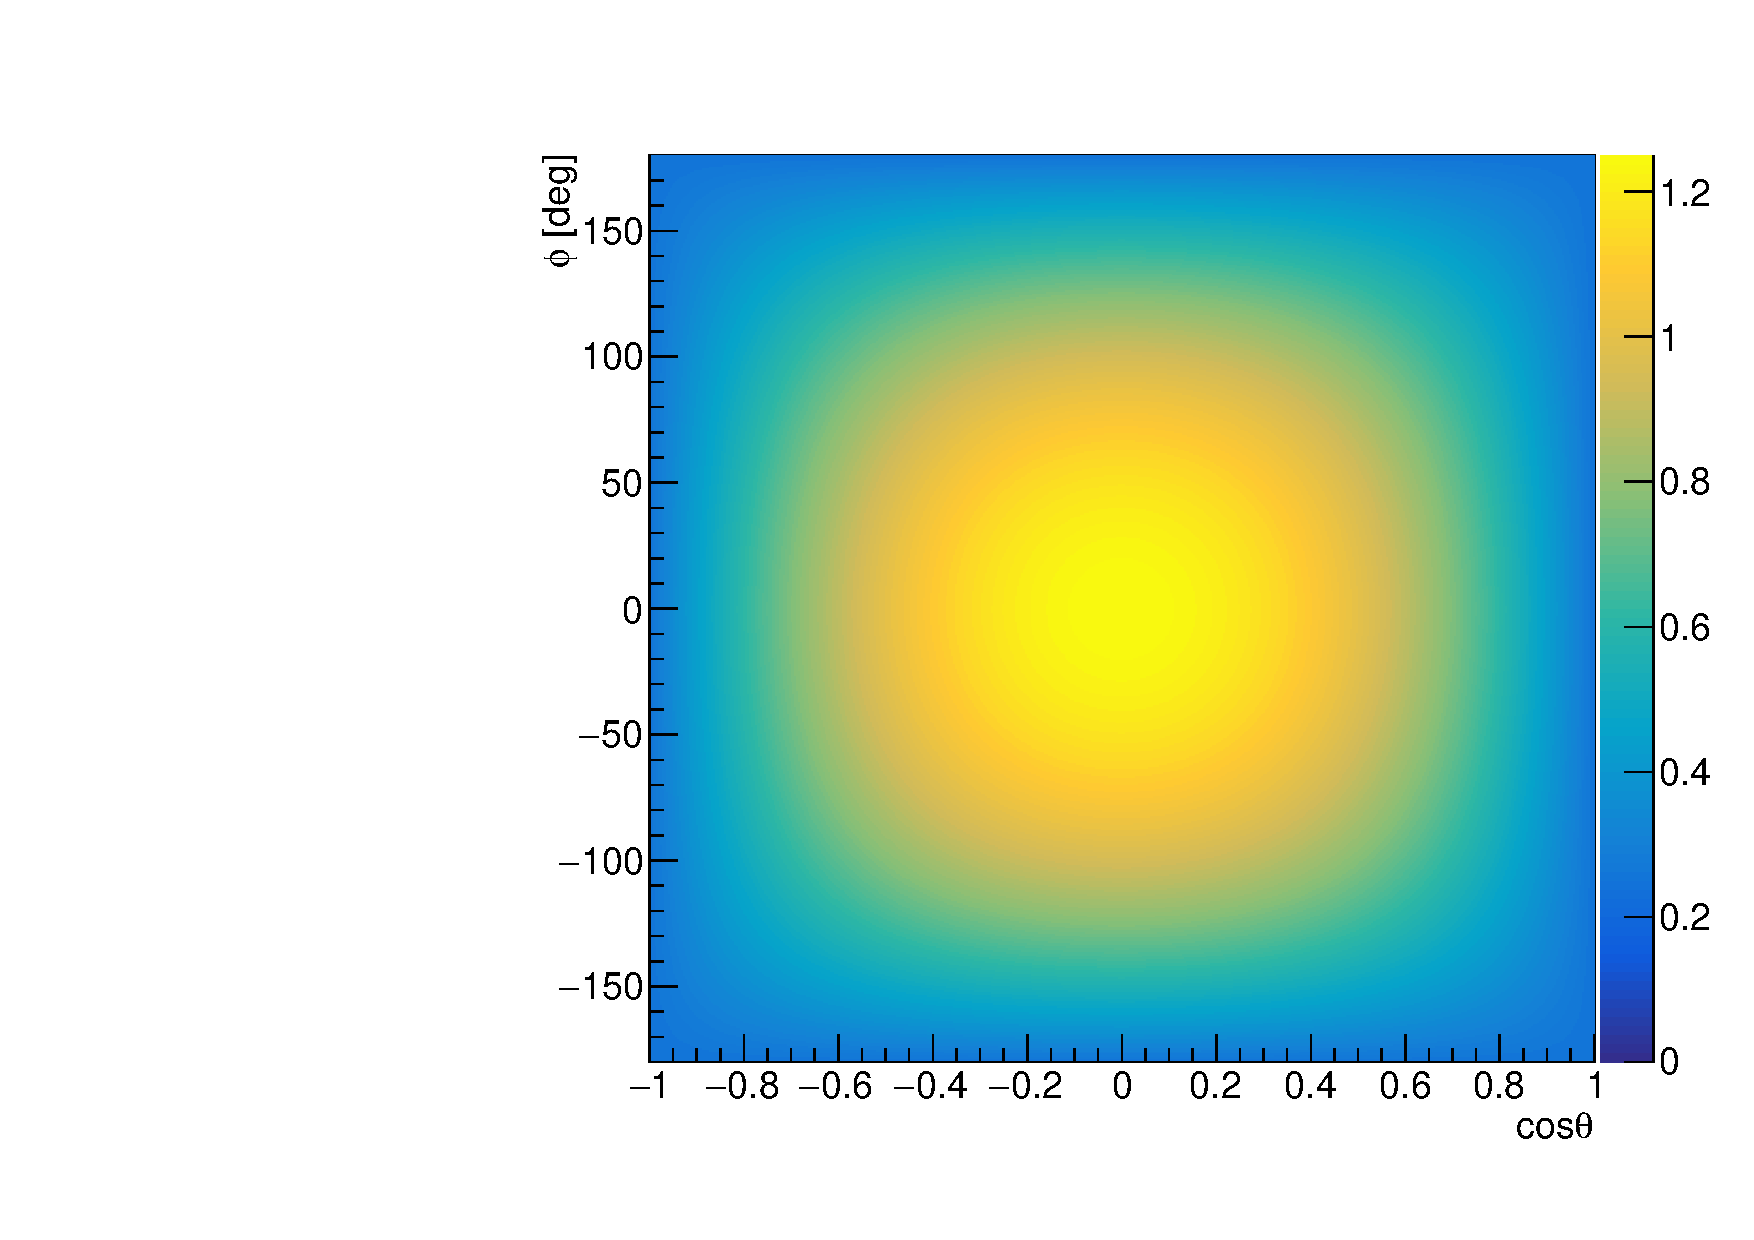
\includegraphics[width=0.5\textwidth]{photoprod/acc_1/hEfficiency}%
  }%
  \\%
  \subfloat[][]{%
    \label{fig:photoprod_study_intensity_acc}%
    \includegraphics[width=0.5\textwidth]{photoprod/acc_1/hIntensity}%
  }%
  \subfloat[][]{%
    \label{fig:photoprod_study_data}%
    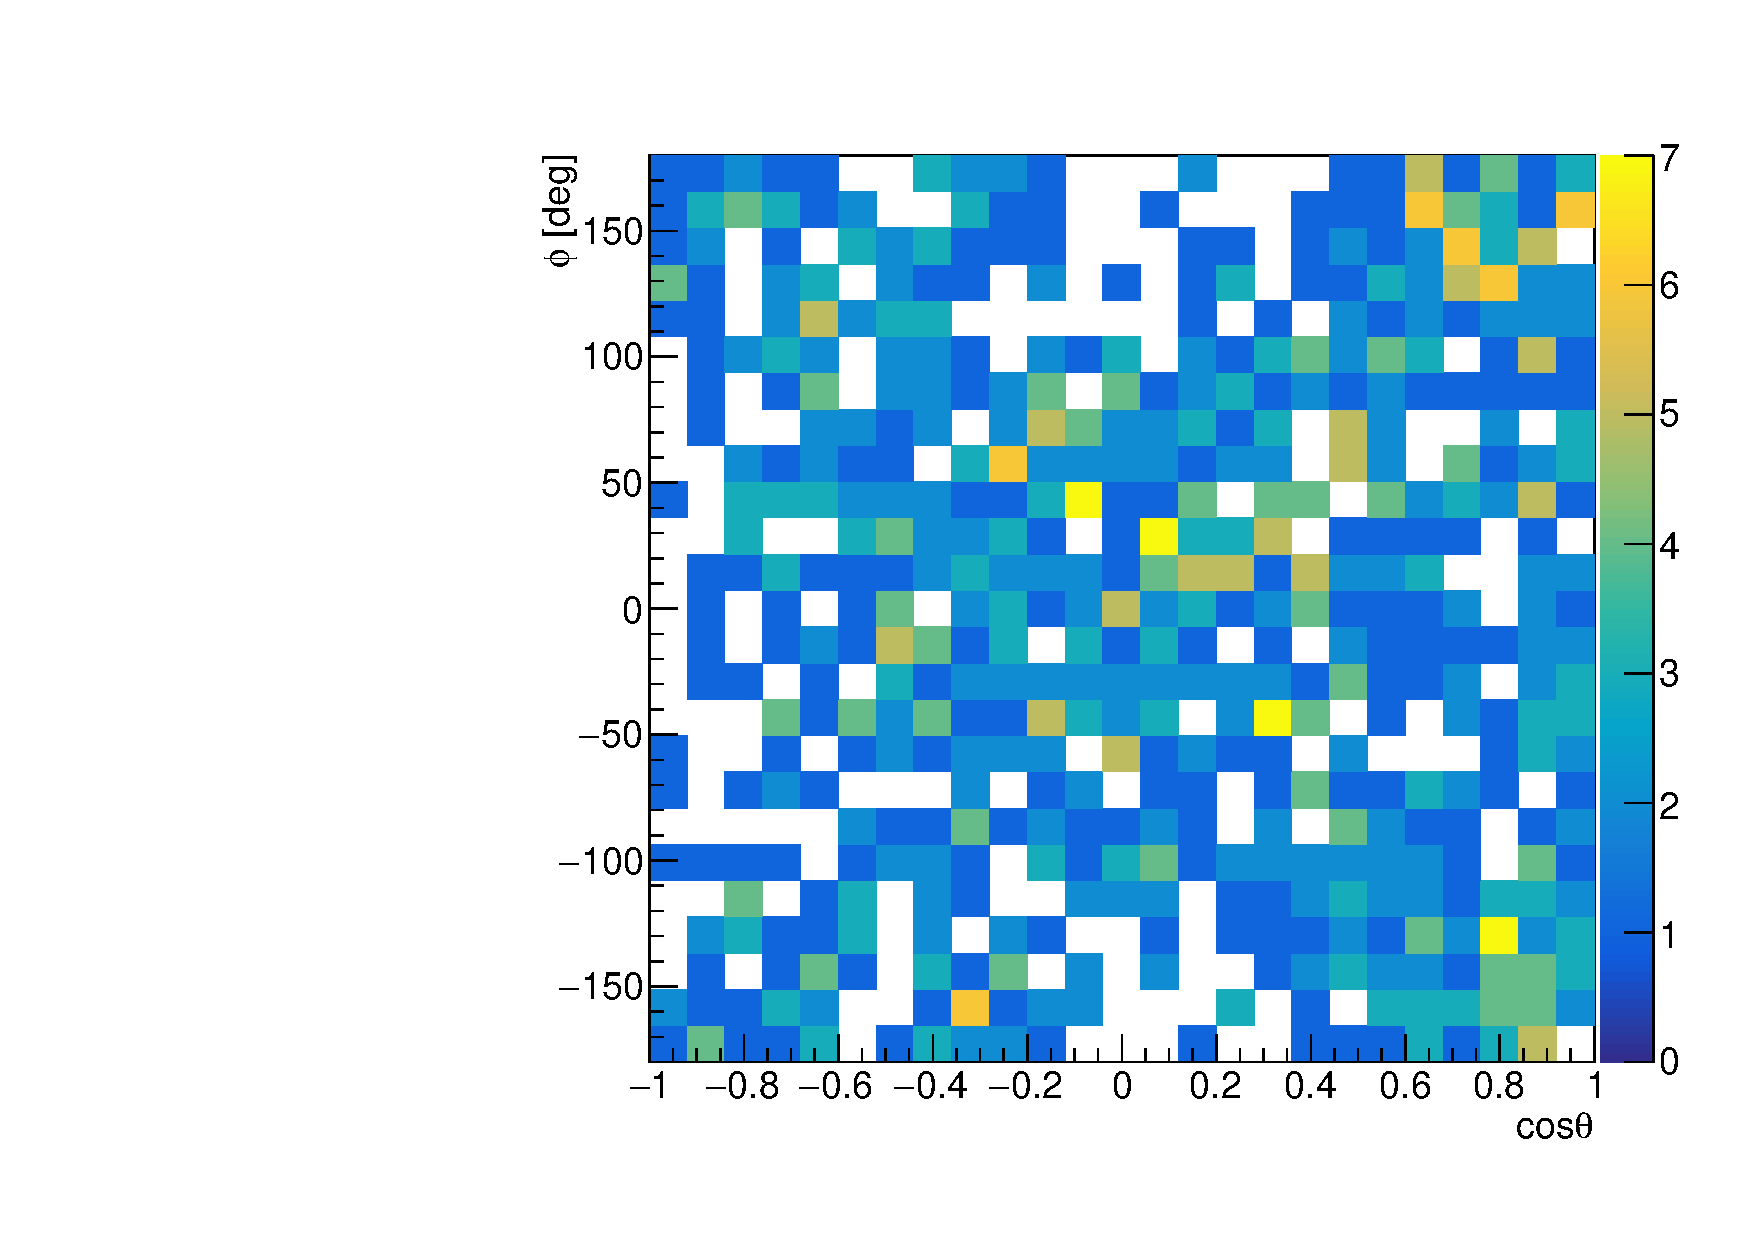
\includegraphics[width=0.5\textwidth]{photoprod/acc_1/hData}%
  }%
  \caption{Input used to generate Monte Carlo data:
  \subfloatLabel{fig:photoprod_study_intensity}~Intensity distribution
  $\intensity(\Omega, \Phi)$ calculated from the partial-wave
  amplitudes listed in \cref{tab:photoprod_study_waveset}.
  \subfloatLabel{fig:photoprod_study_efficiency}~Hypothetical
  detection efficiency $\eta(\Omega, \Phi)$ as given by
  \cref{eq:photoprod_study_acc1}.
  \subfloatLabel{fig:photoprod_study_intensity_acc}~Intensity
  distribution weighted by the detection efficiency, \ie $\eta(\Omega,
  \Phi)\, \intensity(\Omega, \Phi)$.
  \subfloatLabel{fig:photoprod_study_data}~Monte Carlo data sample of
  \num{1000}~events randomly drawn from the distribution
  in~\subfloatLabel{fig:photoprod_study_intensity_acc}.}%
  \label{fig:photoprod_study_input}%
\end{figure}

The acceptance integral matrix~$\mat{I}^\text{acc}$ is calculated
using \cref{eq:photoprod_integral_matrix_mc_weighted} based on \num{e7}~events
that are sampled randomly from the detection efficiency $\eta(\Omega,
\Phi)$ in \cref{eq:photoprod_study_acc1}.  Using~$\mat{I}^\text{acc}$,
the physical moments are calculated from the measured moments using
\cref{eq:diffraction_phys_moments,eq:complex_uncert_prop}.
\Crefrange{fig:photoprod_study_output_H0}{fig:photoprod_study_output_H2}
show the physical moments extracted from the Monte Carlo data in
\cref{fig:photoprod_study_data} and compare them to the expected
moment values calculated from the partial-wave amplitudes in
\cref{tab:photoprod_study_waveset} using
\crefrange{eq:photoprod_moment_0_pw_refl}{eq:photoprod_moment_2_pw_refl}.
As expected, the two sets of values  agree within statistical
uncertainties (see
\cref{fig:photoprod_study_residual_H0_re,fig:photoprod_study_residual_H1_re,fig:photoprod_study_residual_H2_im}).
Since the $H_0(L, M)$ and $H_1(L, M)$ are expected to be real-valued
and $H_2(L, M)$ to be purely imaginary (see
\cref{eq:photoprodP_moments_real_imag}), we also verify that the
imaginary parts of $H_{0, 1}(L, M)$ and the real parts of $H_2(L, M)$
are consistent with zero, which is indeed the case (see
\cref{fig:photoprod_study_comparison_H0_im,fig:photoprod_study_residual_H0_im,fig:photoprod_study_comparison_H1_im,fig:photoprod_study_residual_H1_im,fig:photoprod_study_comparison_H2_re,fig:photoprod_study_residual_H2_re}).

\begin{figure}[tbp]
  \centering%
  \subfloat[][]{%
    \label{fig:photoprod_study_comparison_H0_re}%
    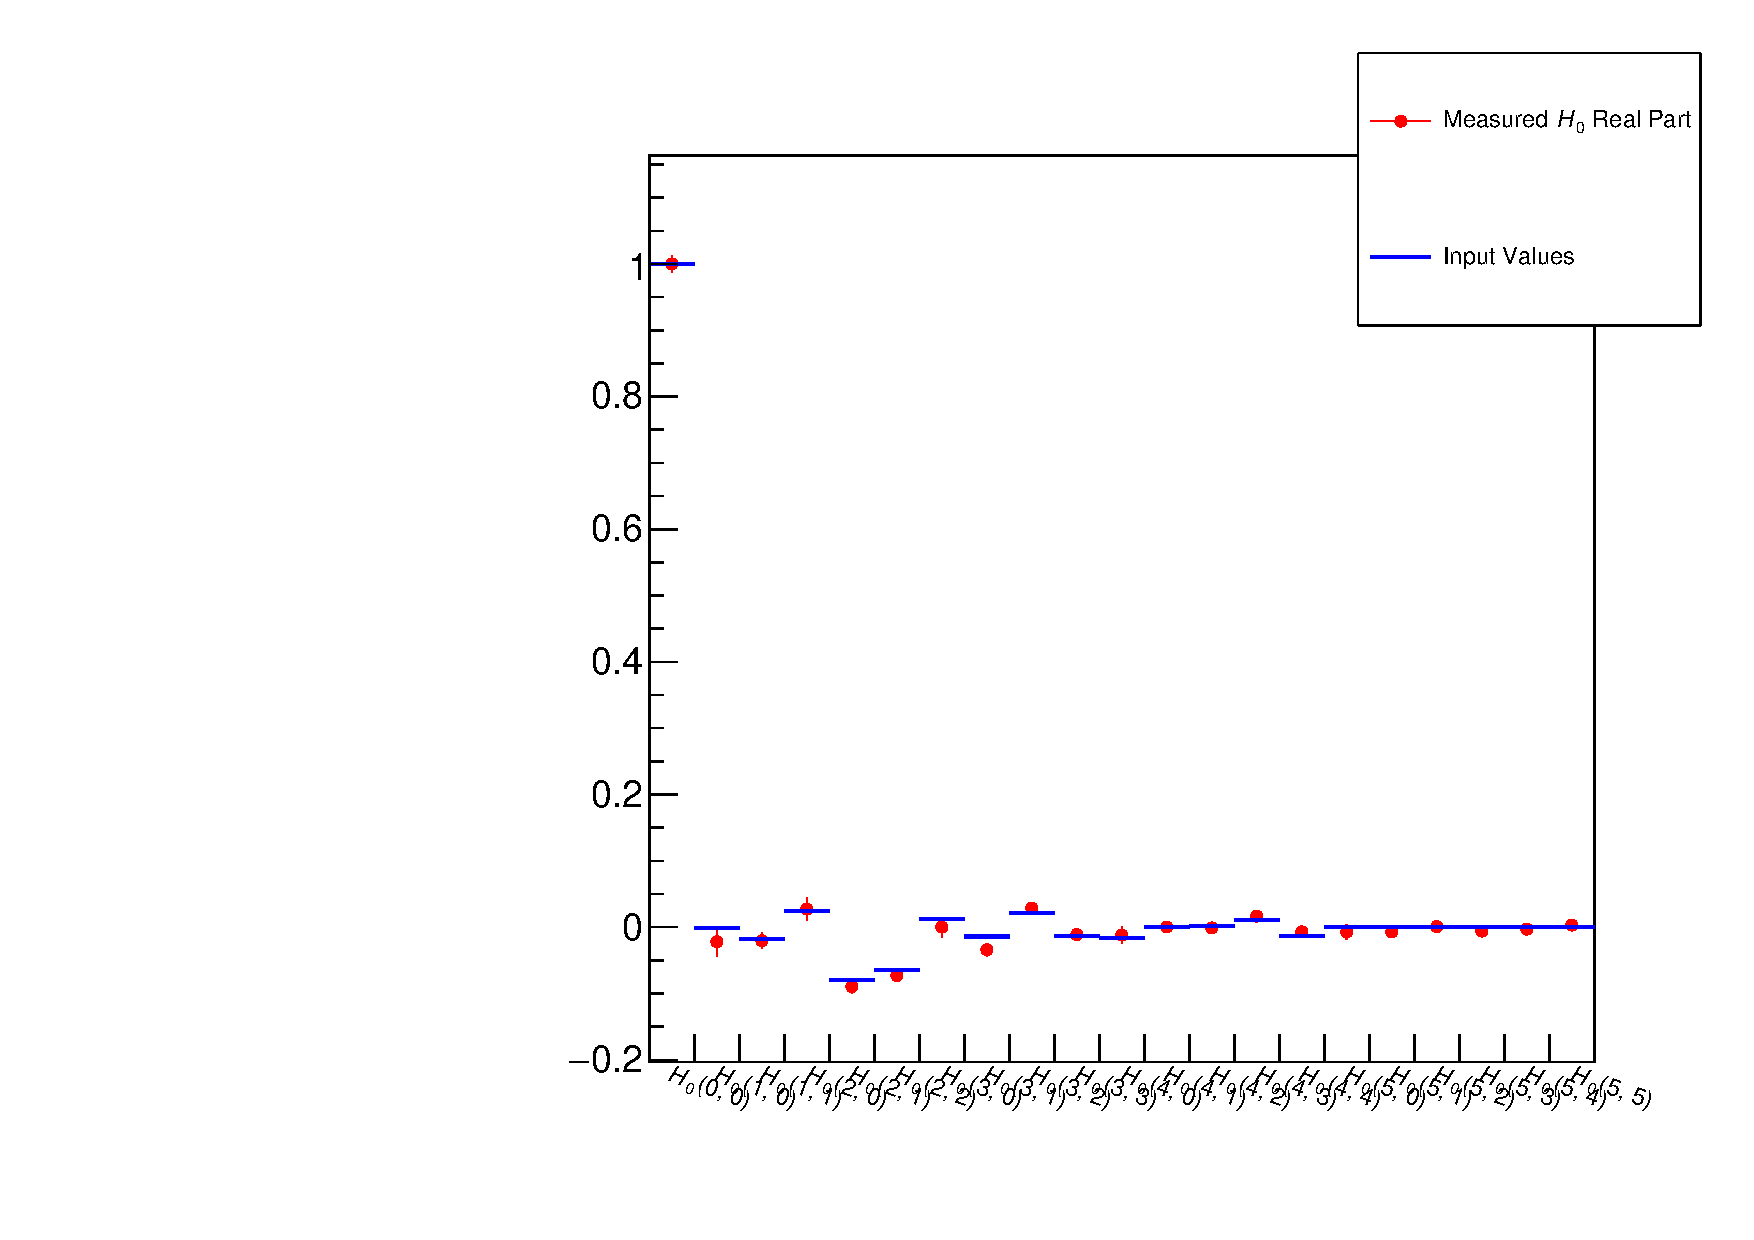
\includegraphics[width=0.5\textwidth]{photoprod/acc_1/hCompare_H0_Re}%
  }%
  \subfloat[][]{%
    \label{fig:photoprod_study_comparison_H0_im}%
    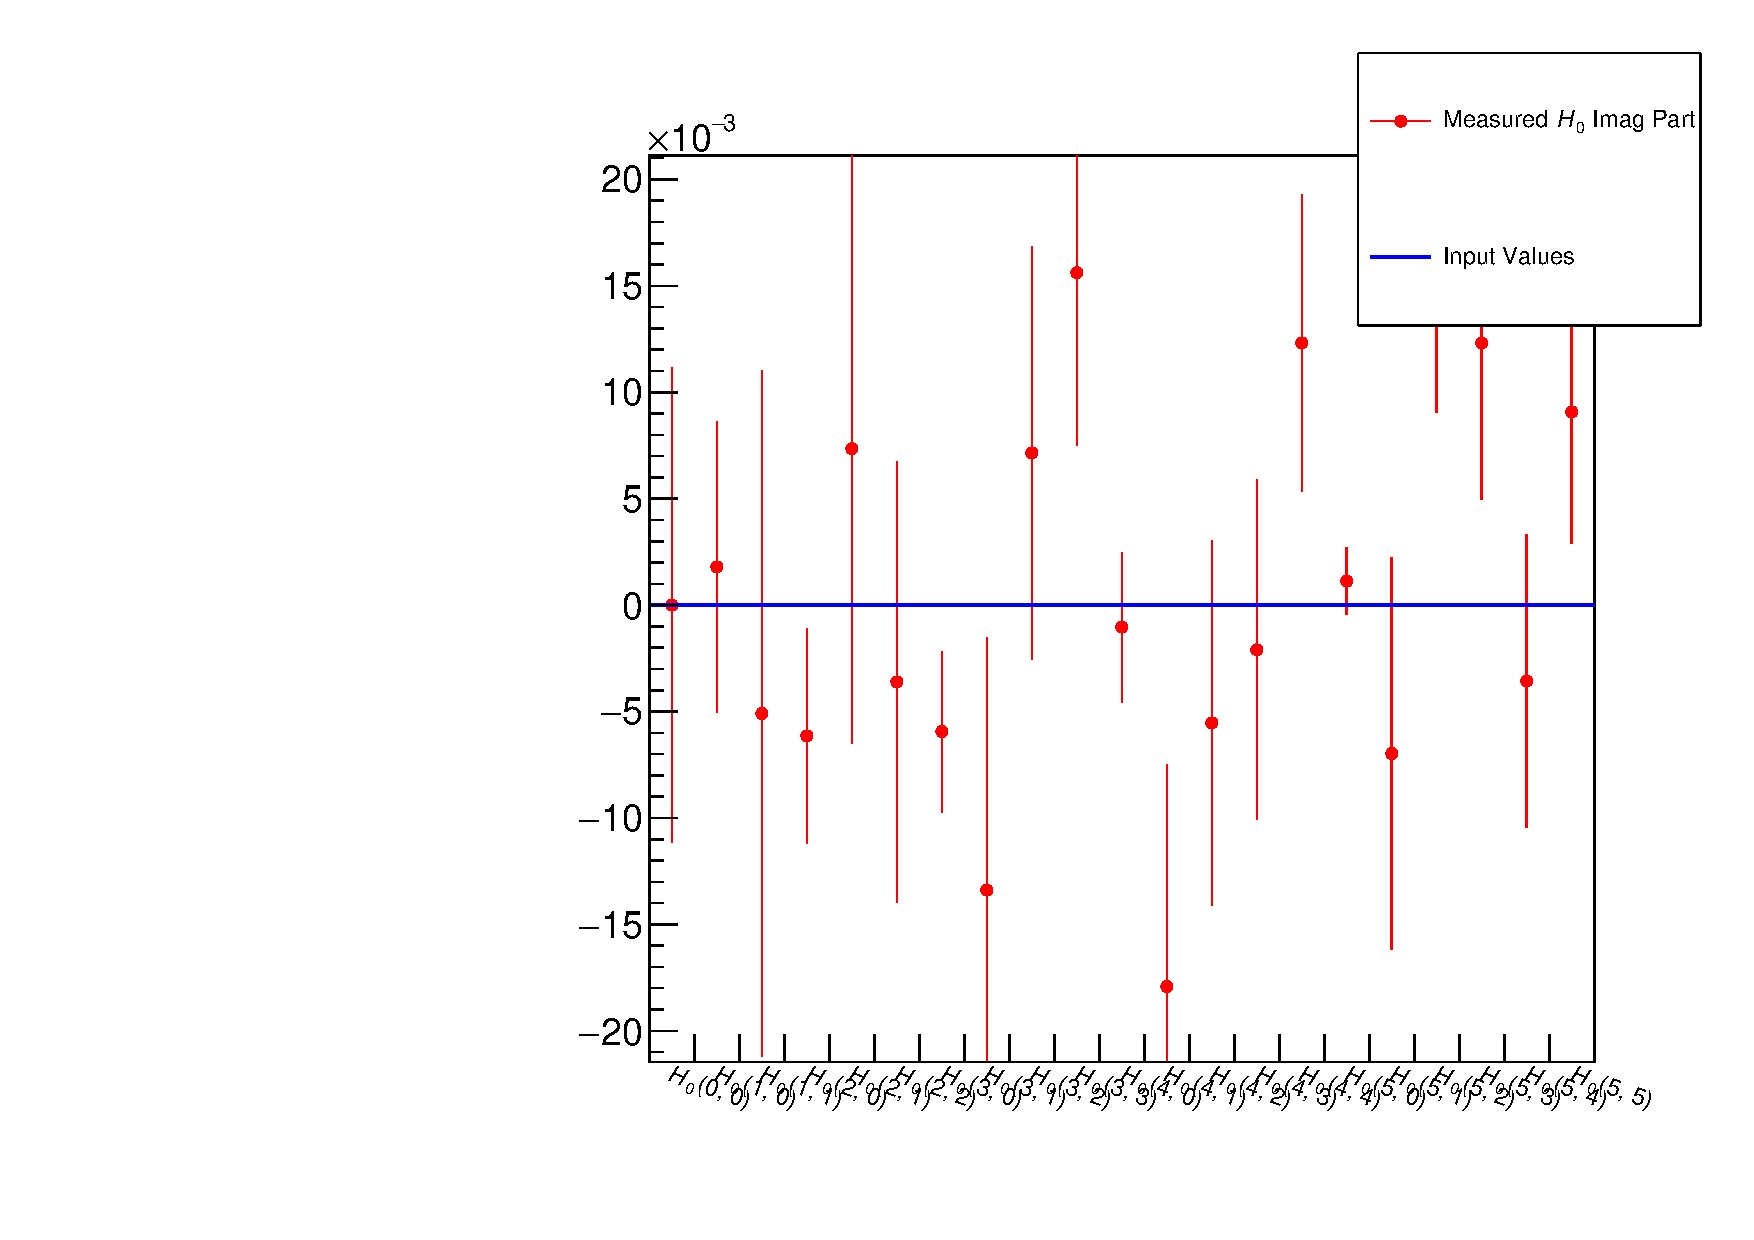
\includegraphics[width=0.5\textwidth]{photoprod/acc_1/hCompare_H0_Im}%
  }%
  \\%
  \subfloat[][]{%
    \label{fig:photoprod_study_residual_H0_re}%
    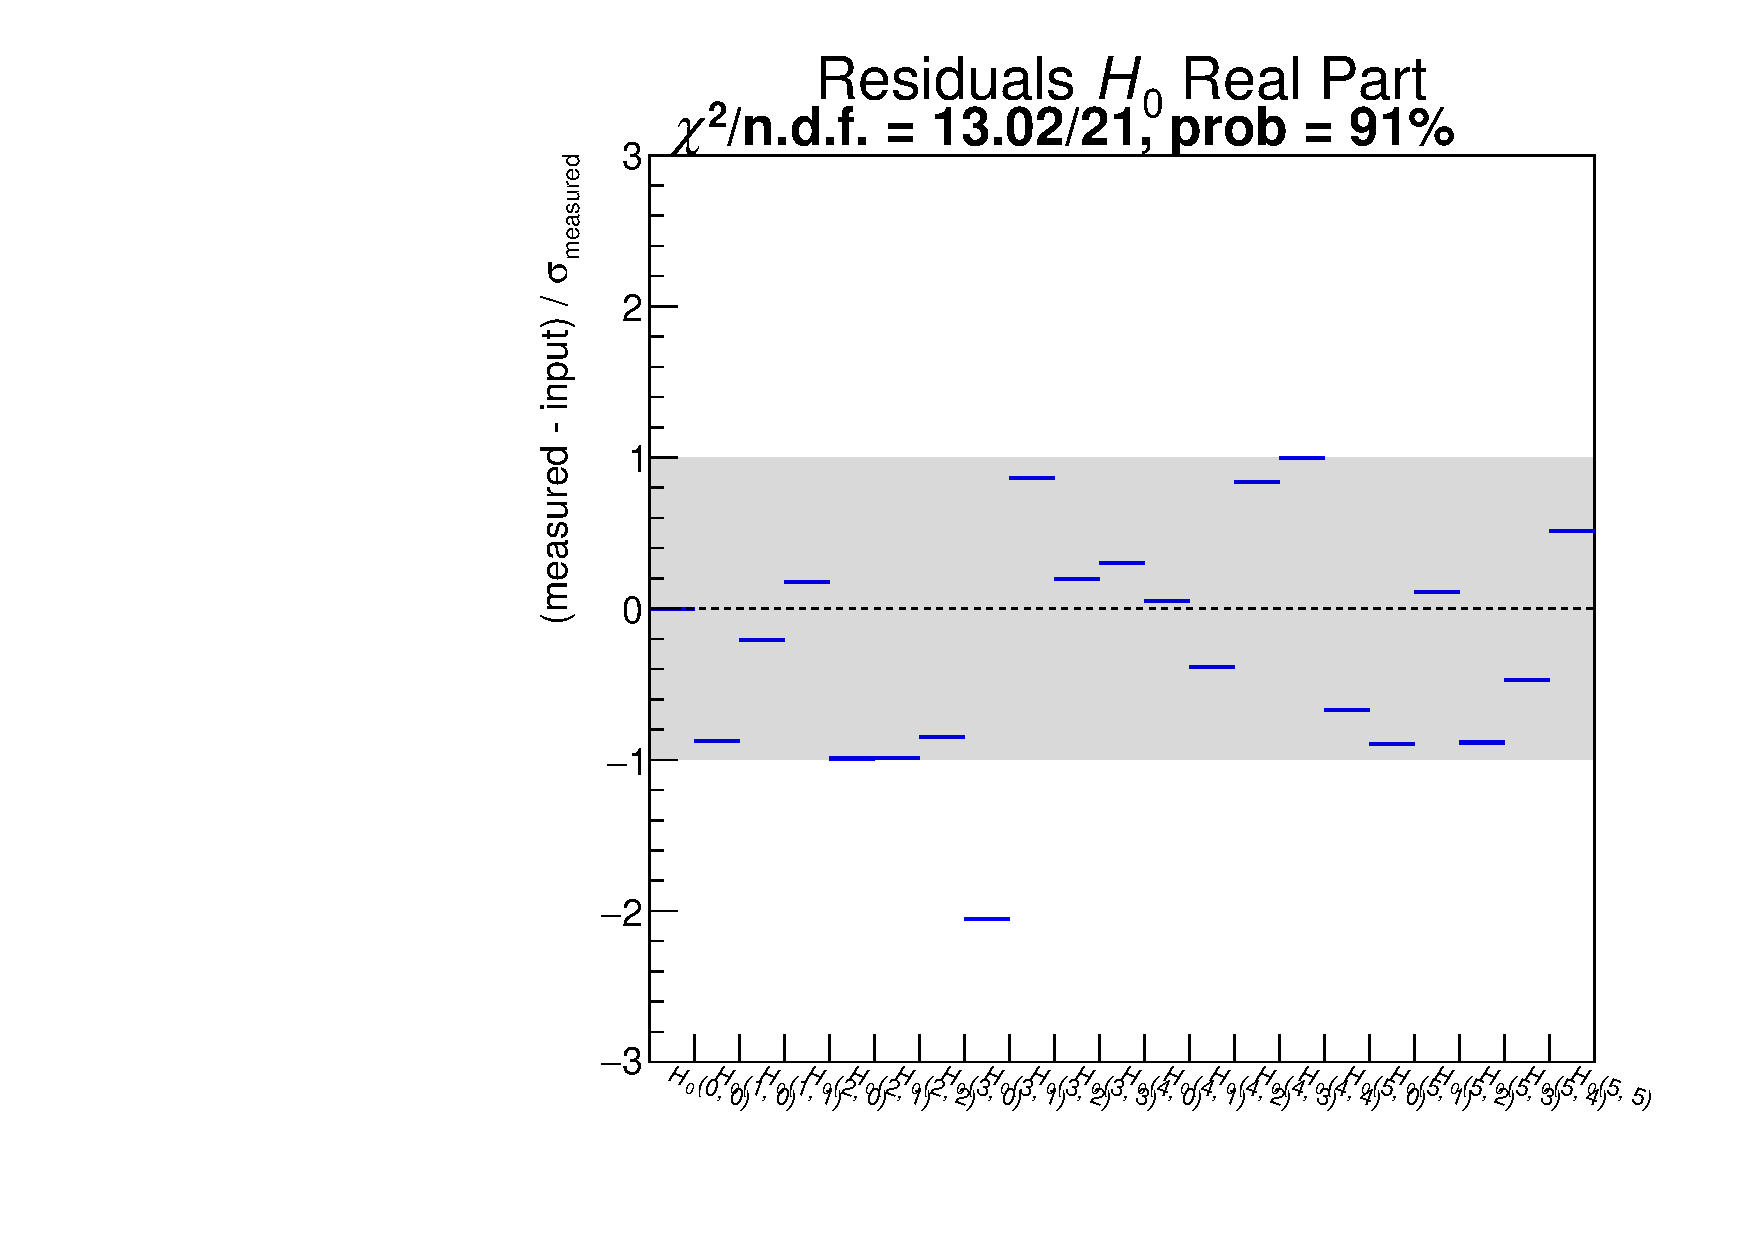
\includegraphics[width=0.5\textwidth]{photoprod/acc_1/hResiduals_H0_Re}%
  }%
  \subfloat[][]{%
    \label{fig:photoprod_study_residual_H0_im}%
    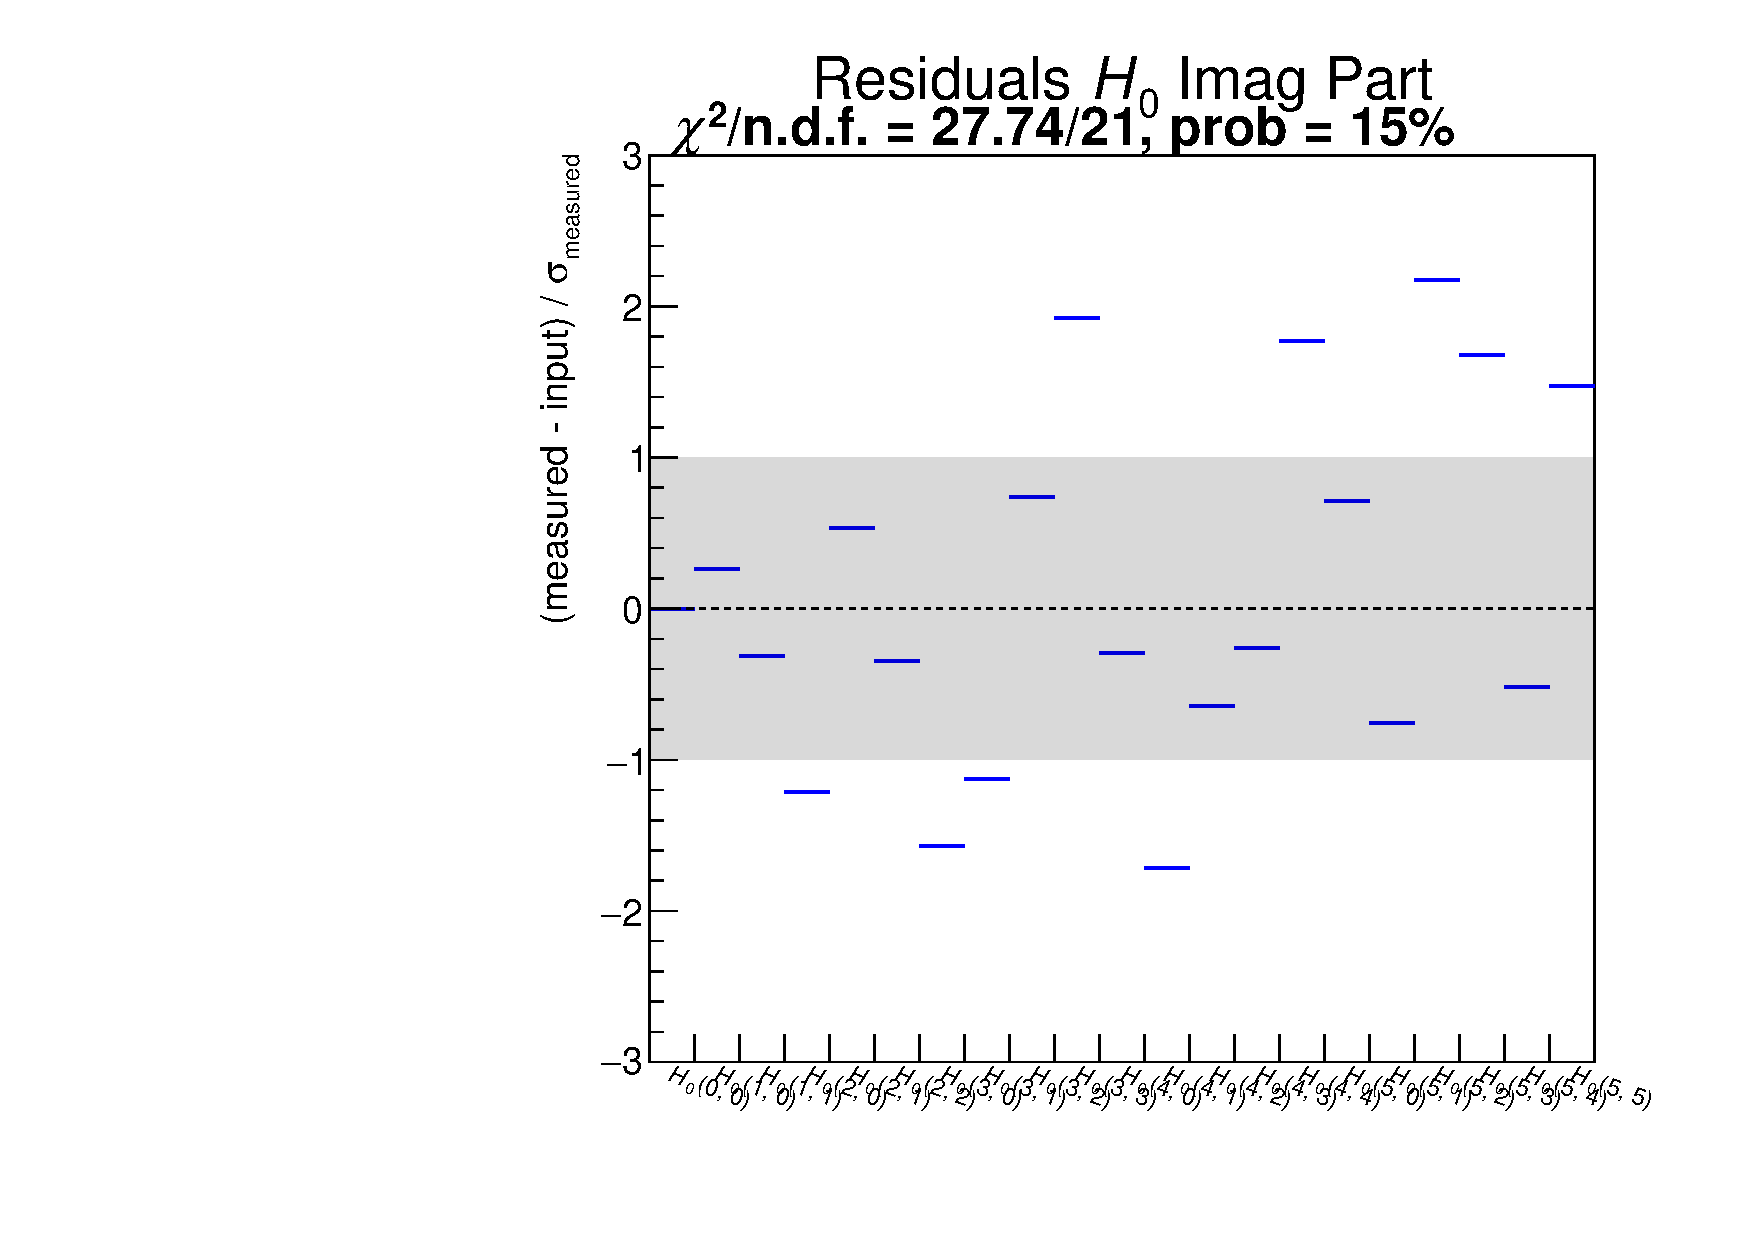
\includegraphics[width=0.5\textwidth]{photoprod/acc_1/hResiduals_H0_Im}%
  }%
  \caption{Upper row: Comparison of the physical moments $H_0(L, M)$
  (red points with uncertainties) extracted from the Monte Carlo data,
  which are generated using the partial-wave amplitudes in
  \cref{tab:photoprod_study_waveset} and the detection efficiency in
  \cref{eq:photoprod_study_acc1}, with the expected values (blue
  lines).  Both sets of values are normalized to the value of $H_0(0,
  0)$ in the respective set.
  \subfloatLabel{fig:photoprod_study_comparison_H0_re}~shows the real
  part of $H_0(L, M)$,
  \subfloatLabel{fig:photoprod_study_comparison_H0_im}~the imaginary
  part.  Note that moments with $L > 4$ are expected to be zero due to
  the chosen wave set.  Lower row: corresponding residuals.}%
  \label{fig:photoprod_study_output_H0}%
\end{figure}

\begin{figure}[tbp]
  \centering%
  \subfloat[][]{%
    \label{fig:photoprod_study_comparison_H1_re}%
    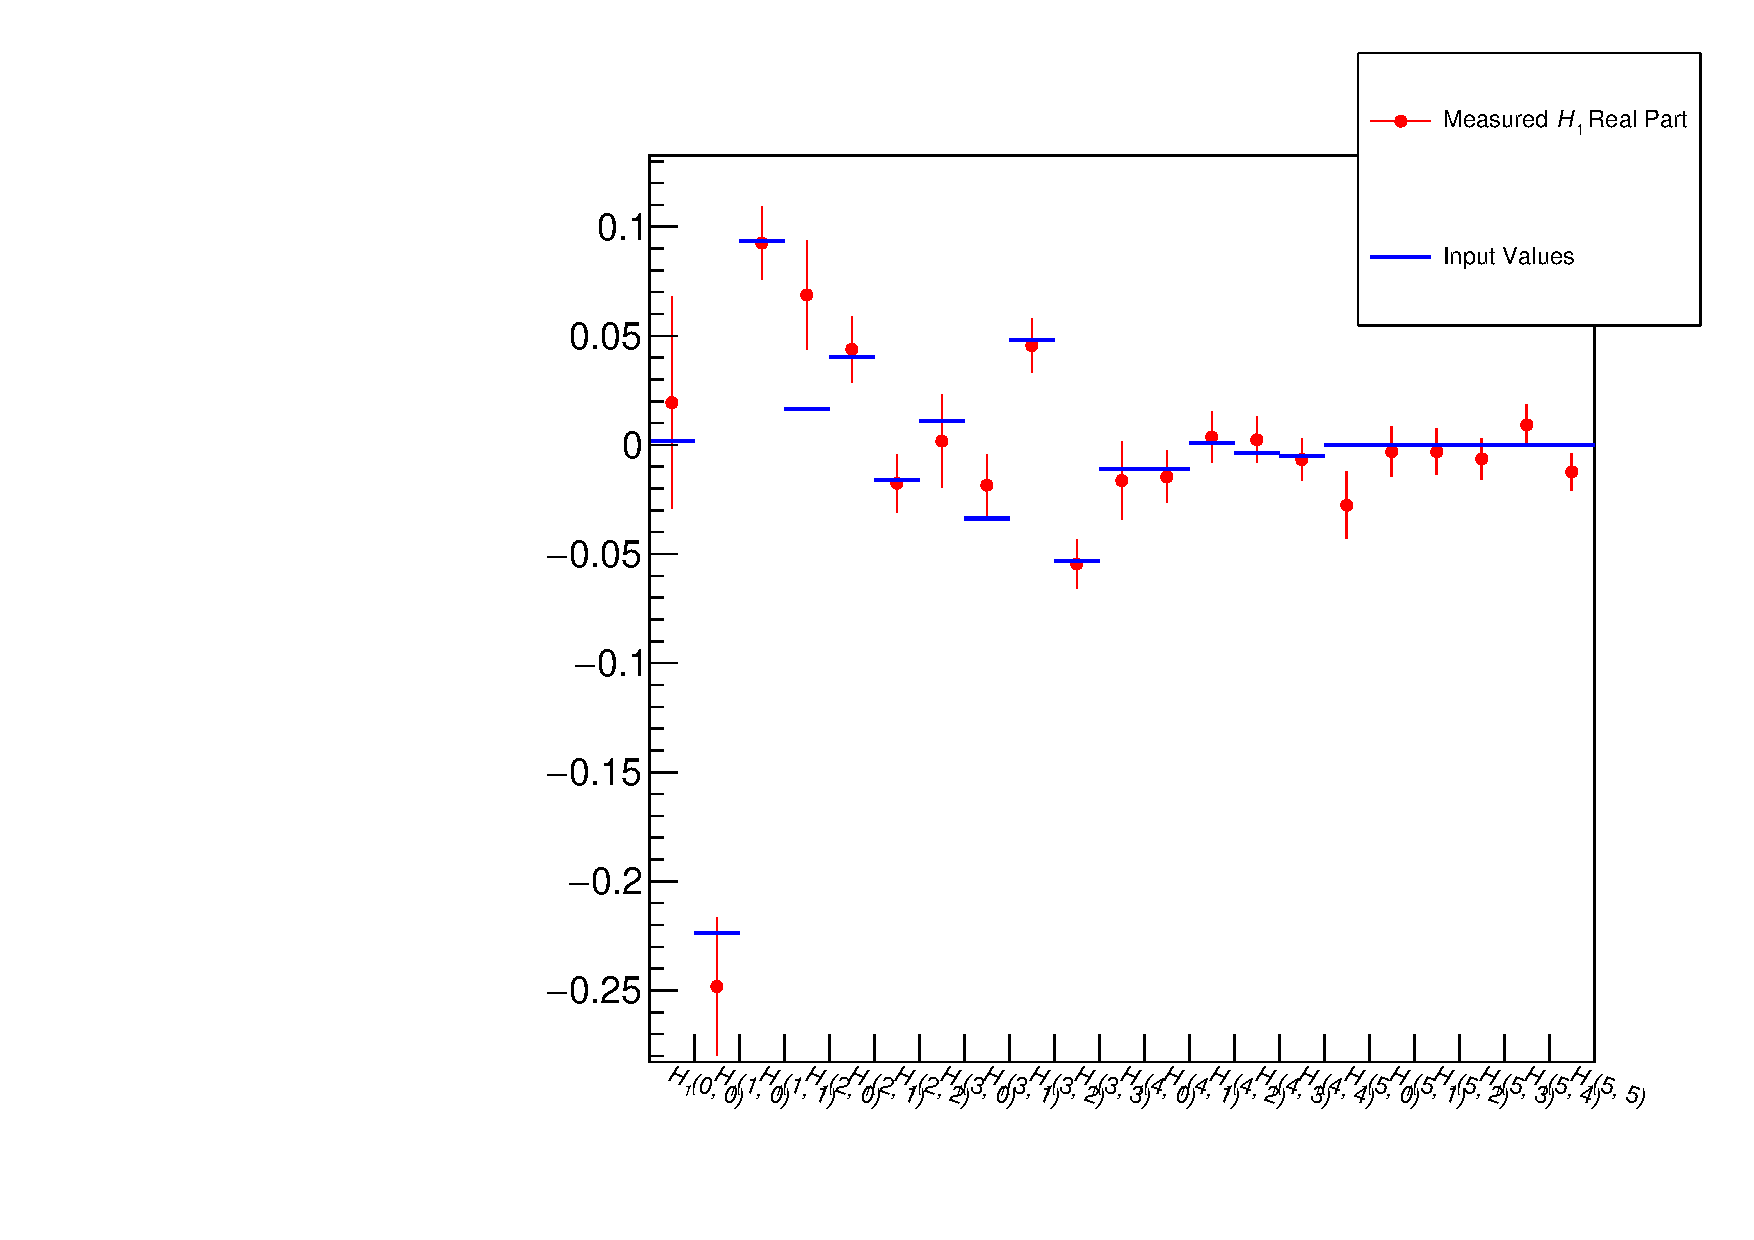
\includegraphics[width=0.5\textwidth]{photoprod/acc_1/hCompare_H1_Re}%
  }%
  \subfloat[][]{%
    \label{fig:photoprod_study_comparison_H1_im}%
    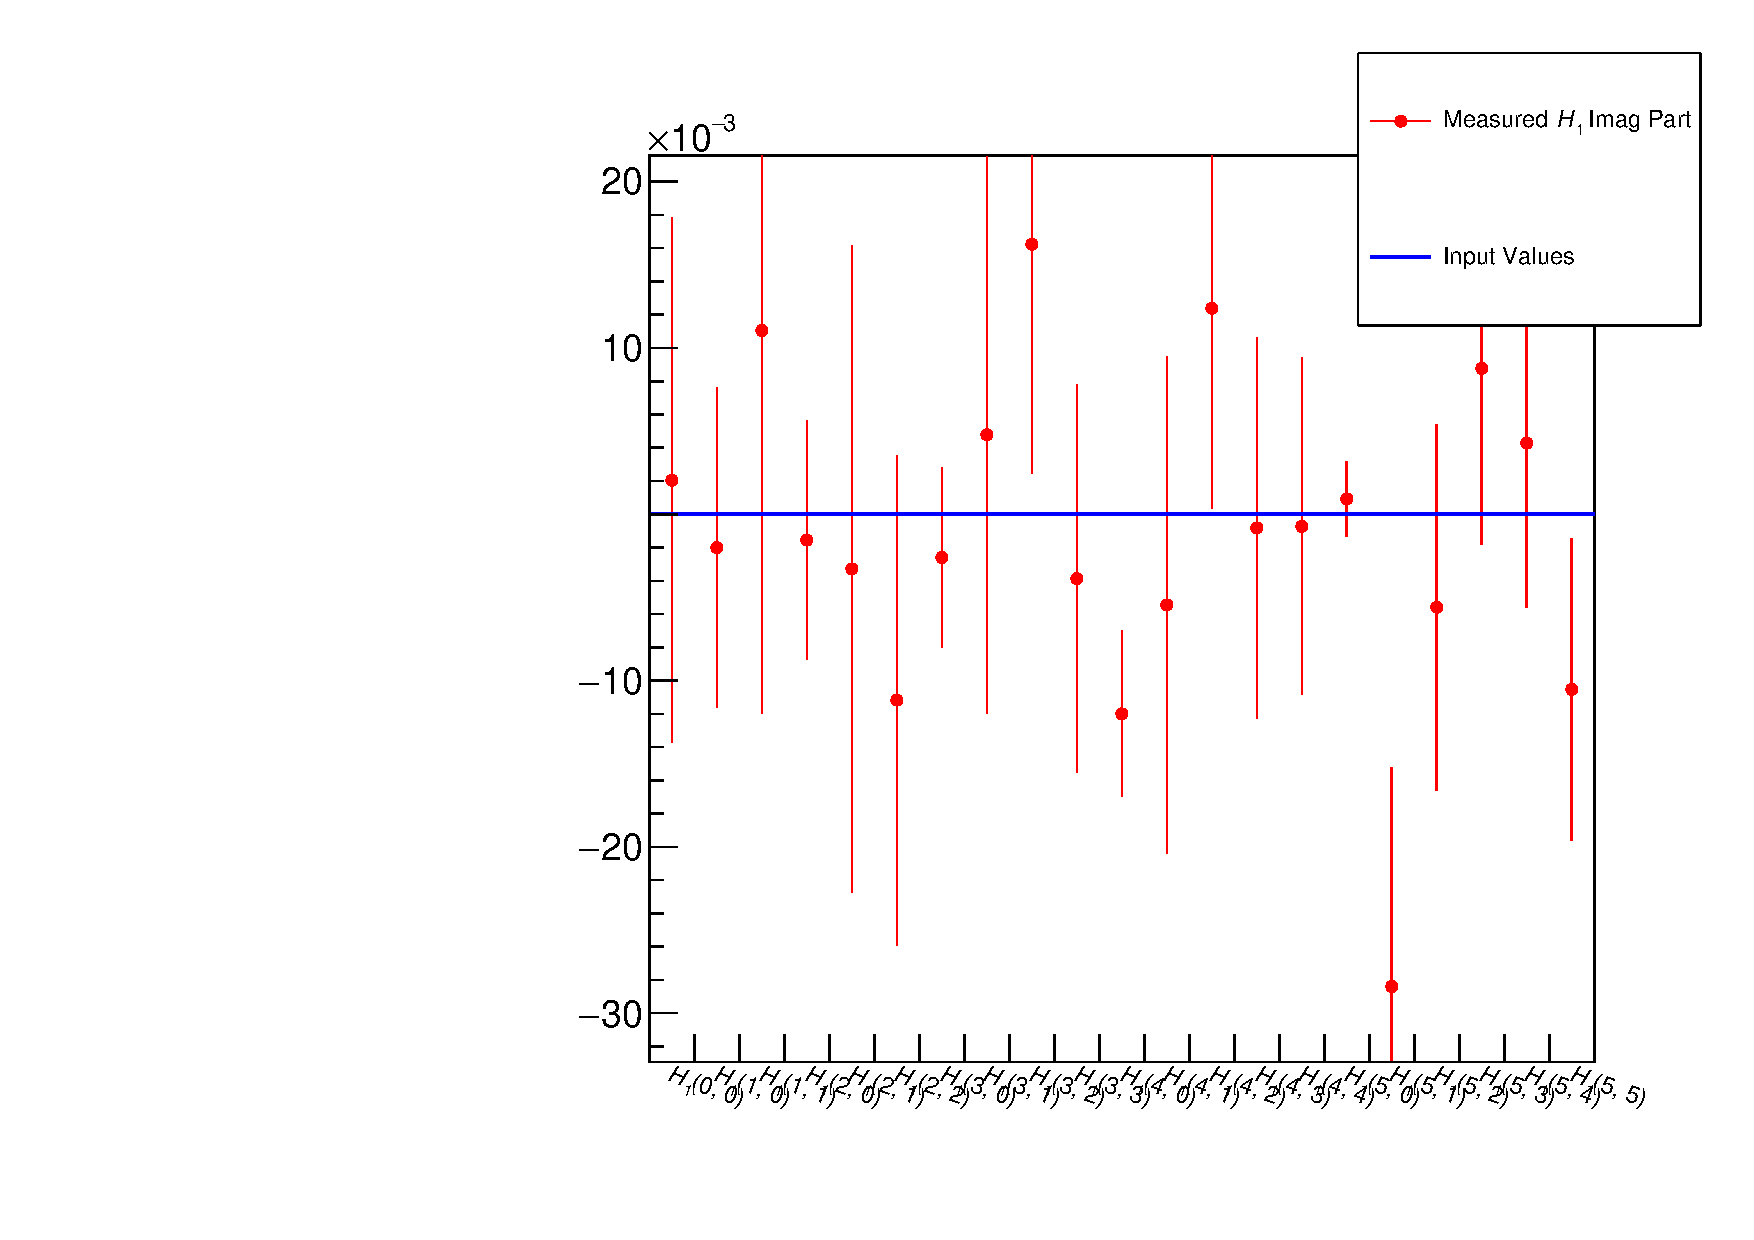
\includegraphics[width=0.5\textwidth]{photoprod/acc_1/hCompare_H1_Im}%
  }%
  \\%
  \subfloat[][]{%
    \label{fig:photoprod_study_residual_H1_re}%
    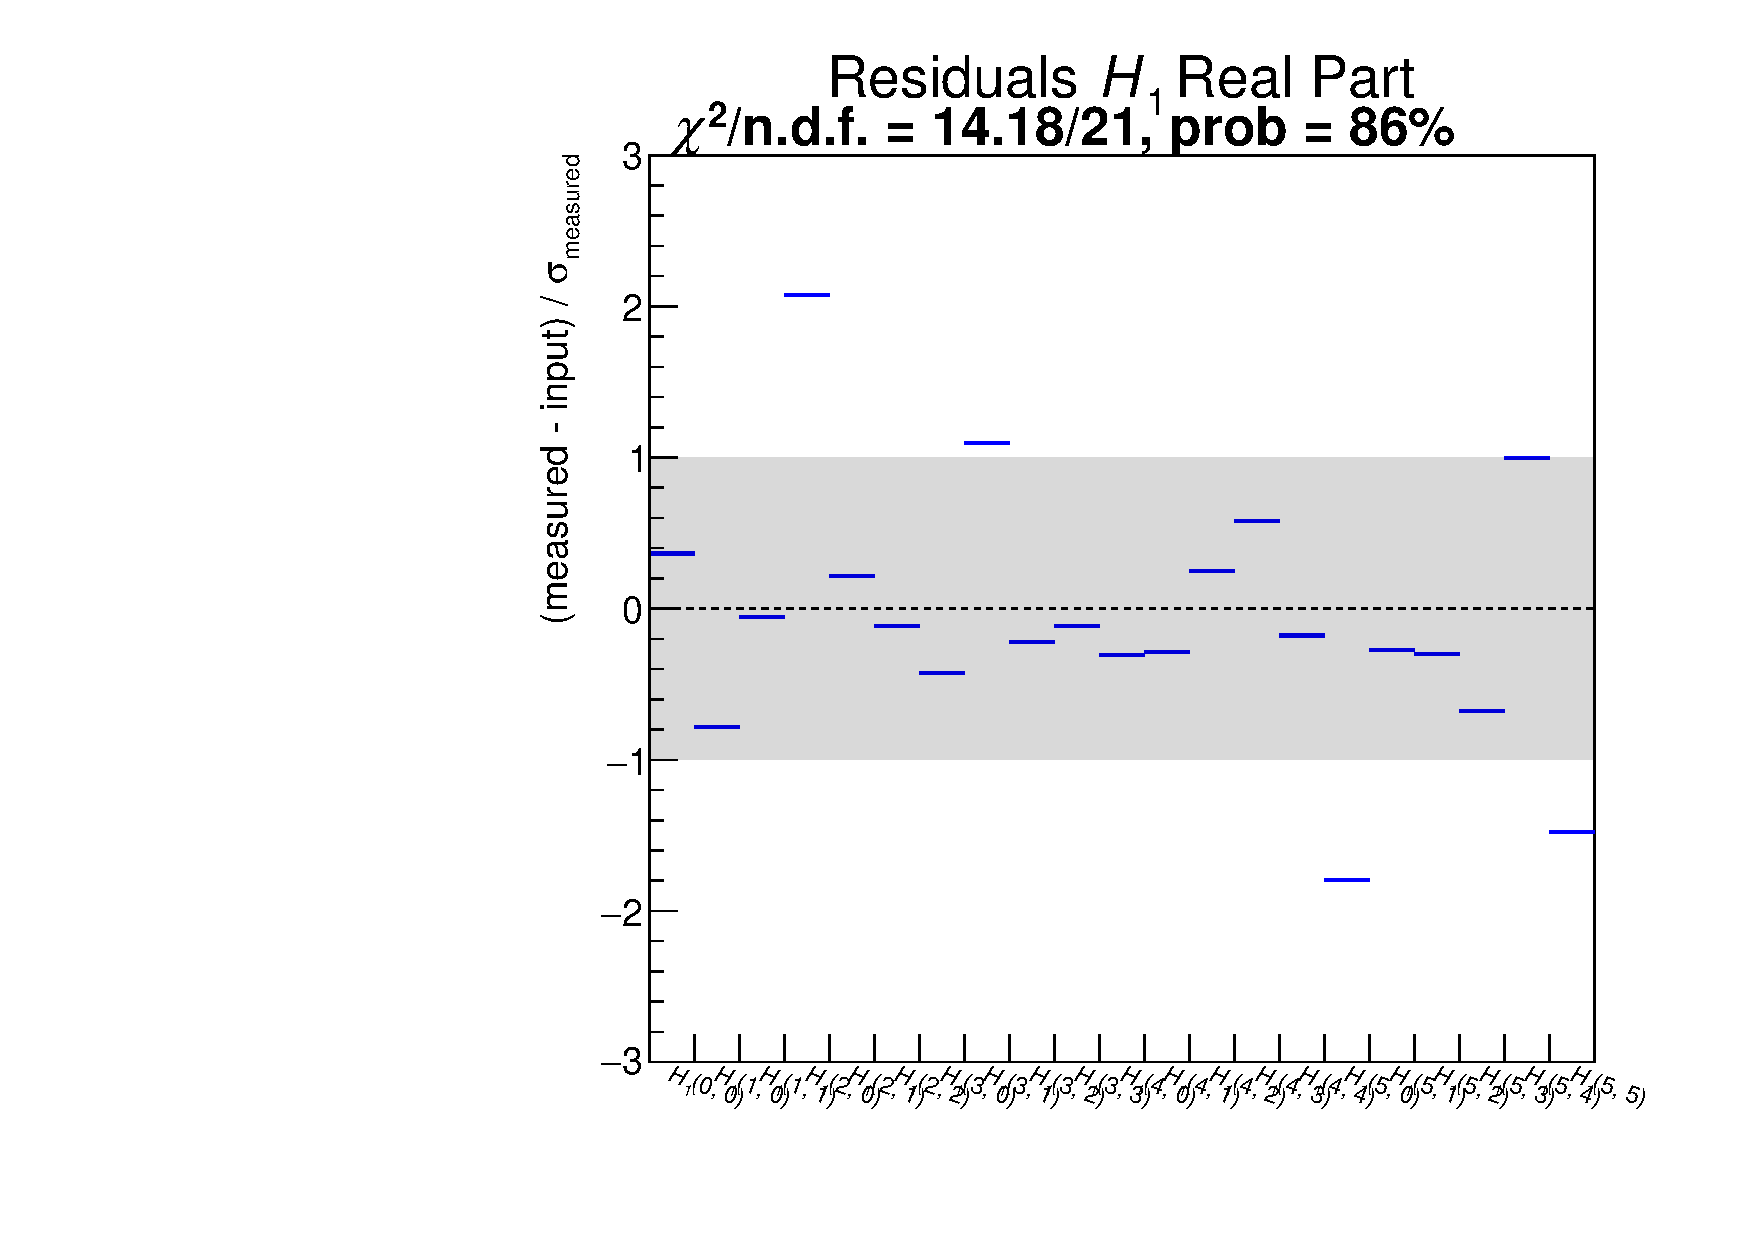
\includegraphics[width=0.5\textwidth]{photoprod/acc_1/hResiduals_H1_Re}%
  }%
  \subfloat[][]{%
    \label{fig:photoprod_study_residual_H1_im}%
    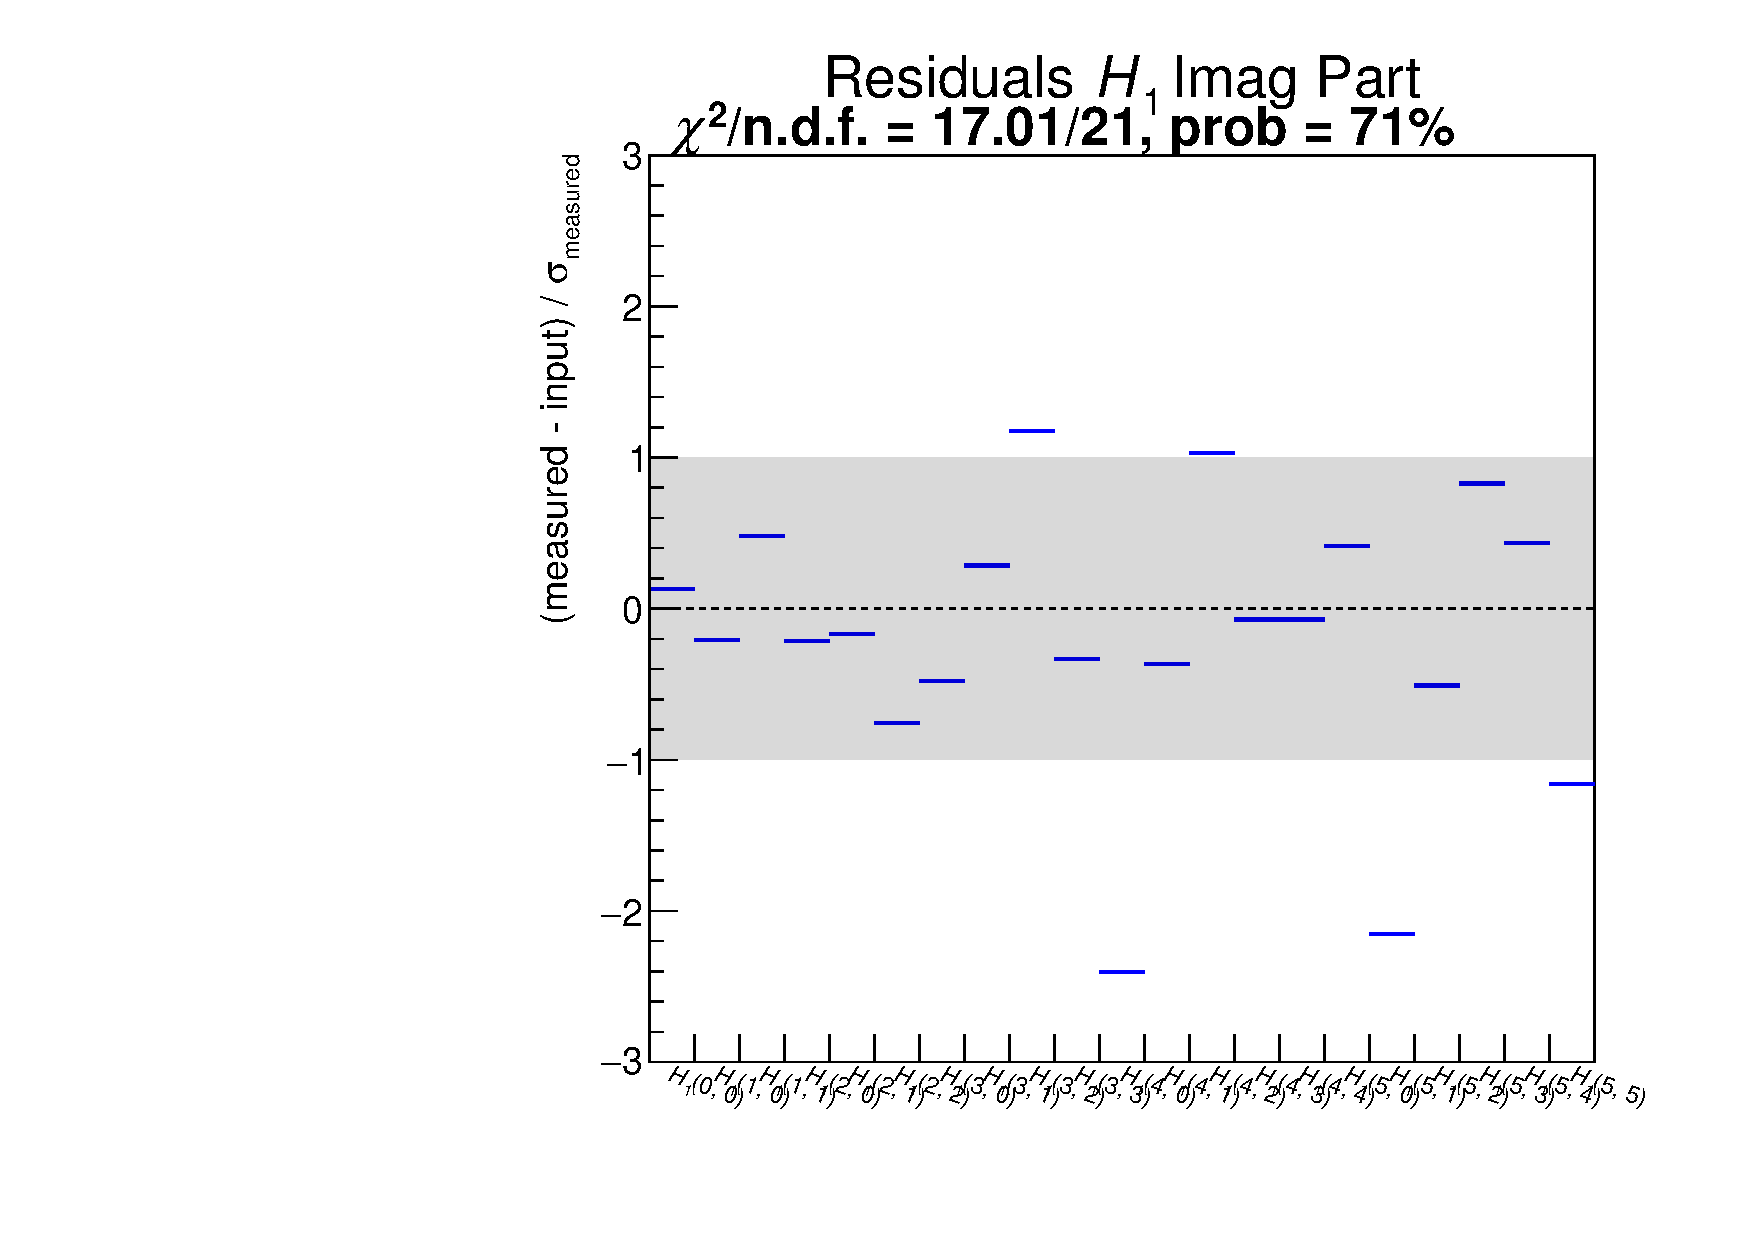
\includegraphics[width=0.5\textwidth]{photoprod/acc_1/hResiduals_H1_Im}%
  }%
  \caption{Same as \cref{fig:photoprod_study_output_H0} but for
  $H_1(L, M)$.}%
  \label{fig:photoprod_study_output_H1}%
\end{figure}

\begin{figure}[tbp]
  \centering%
  \subfloat[][]{%
    \label{fig:photoprod_study_comparison_H2_re}%
    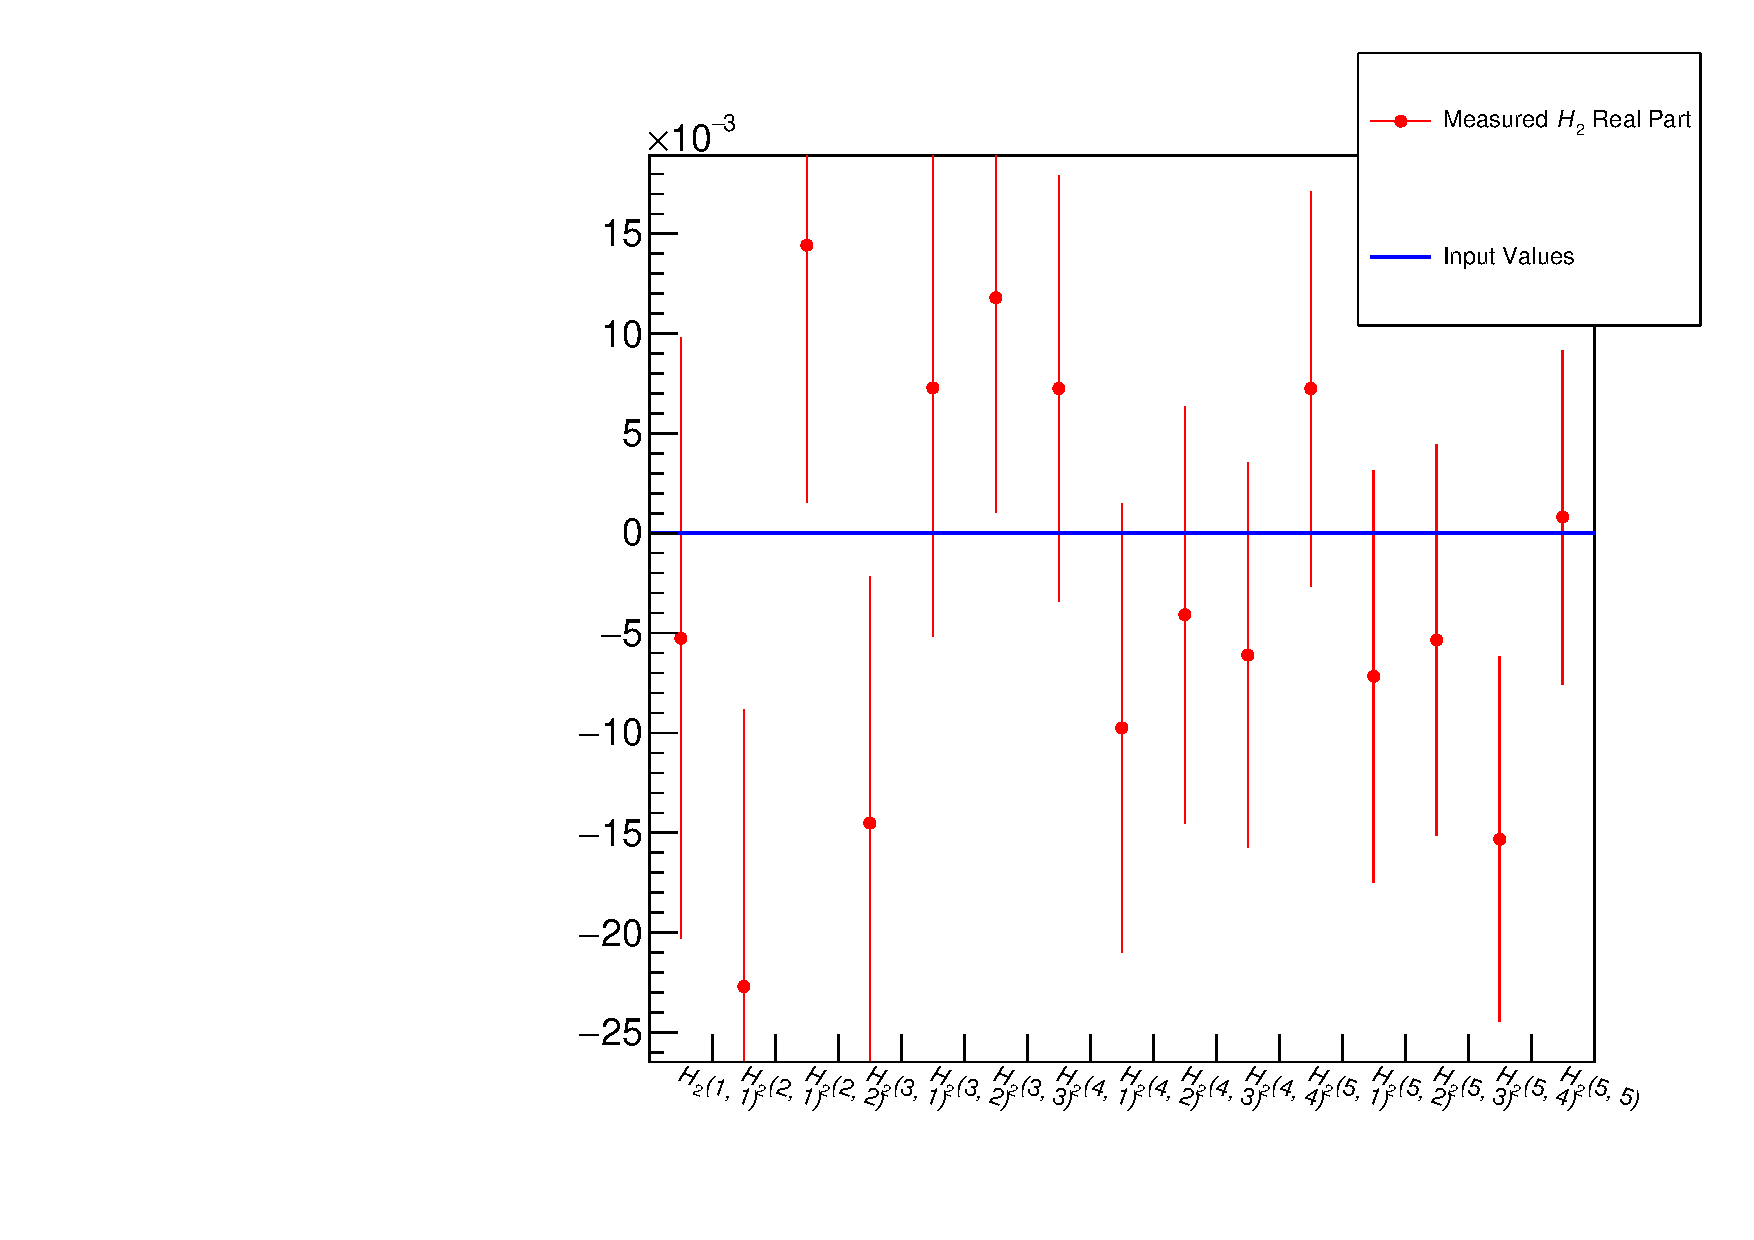
\includegraphics[width=0.5\textwidth]{photoprod/acc_1/hCompare_H2_Re}%
  }%
  \subfloat[][]{%
    \label{fig:photoprod_study_comparison_H2_im}%
    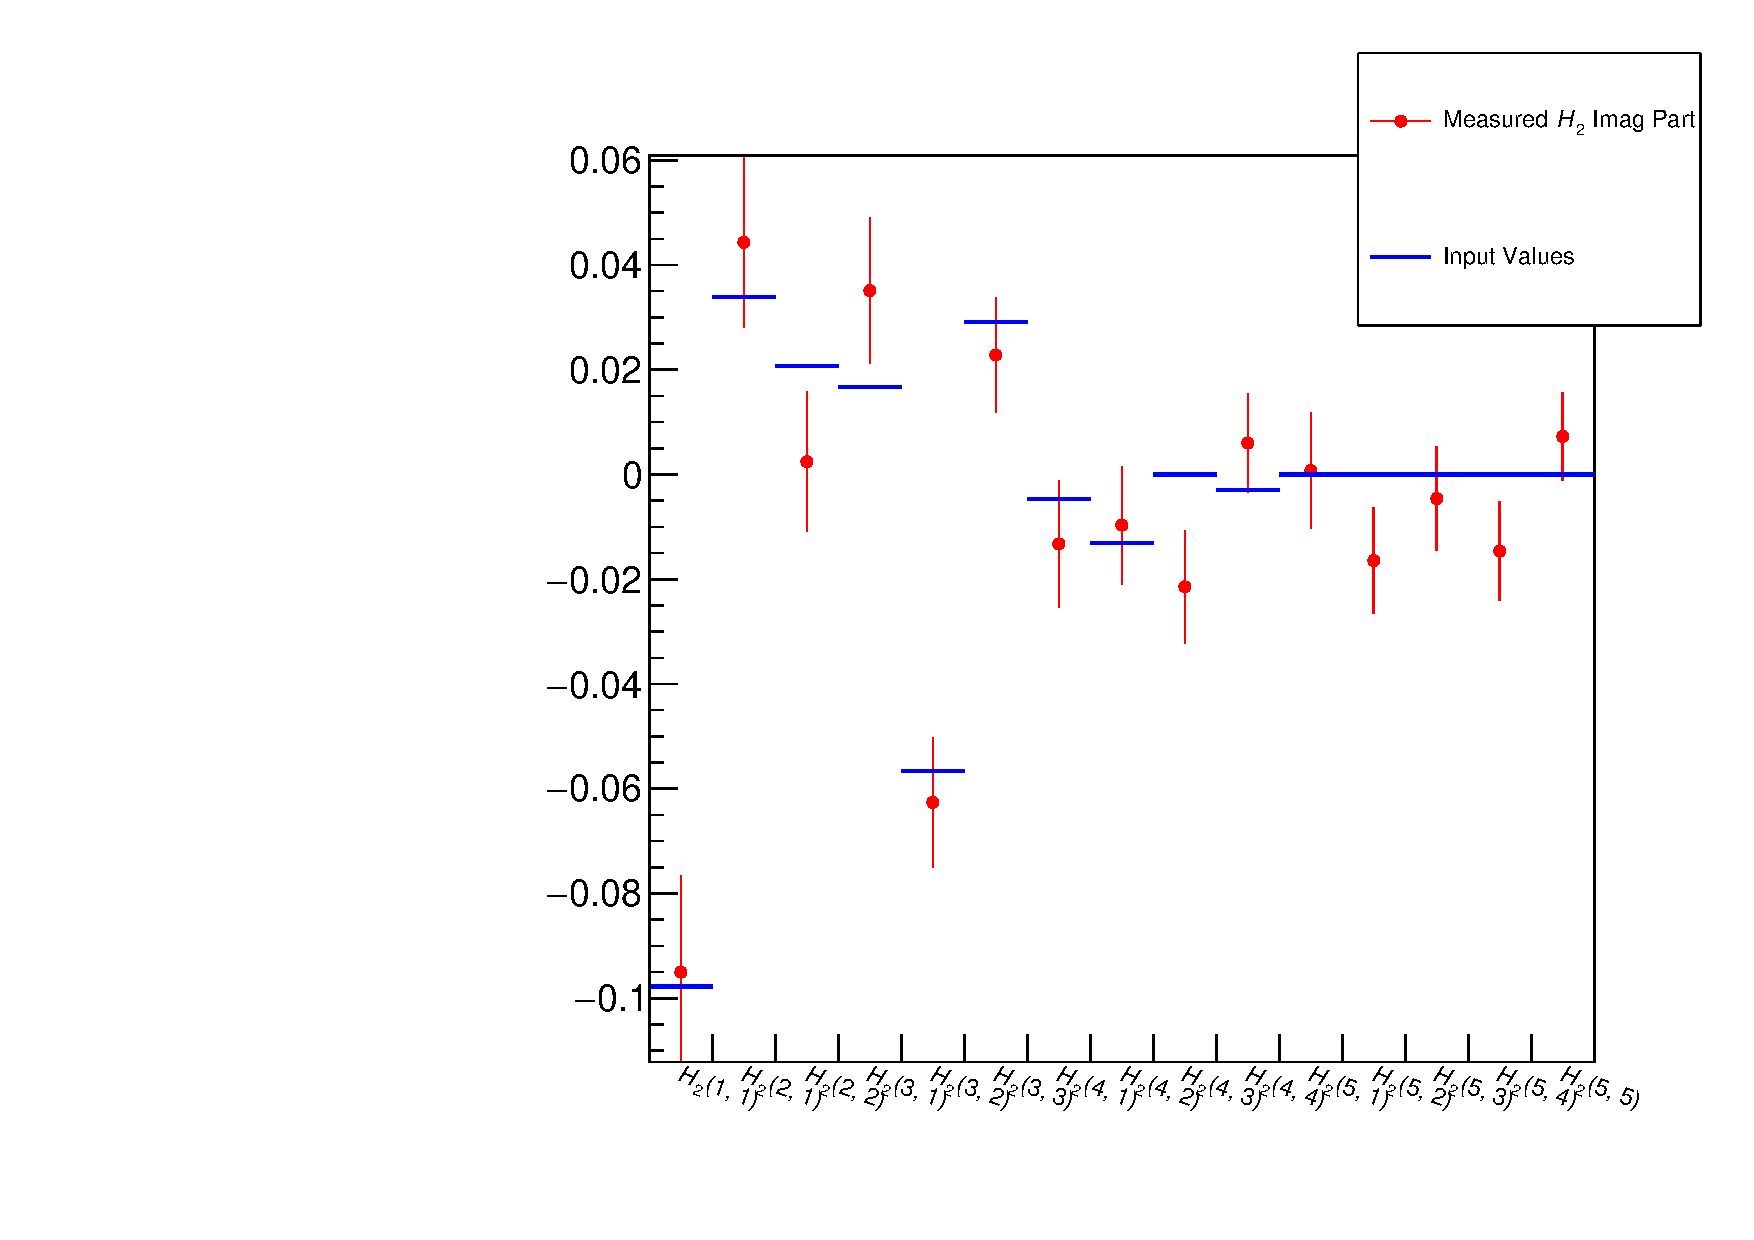
\includegraphics[width=0.5\textwidth]{photoprod/acc_1/hCompare_H2_Im}%
  }%
  \\%
  \subfloat[][]{%
    \label{fig:photoprod_study_residual_H2_re}%
    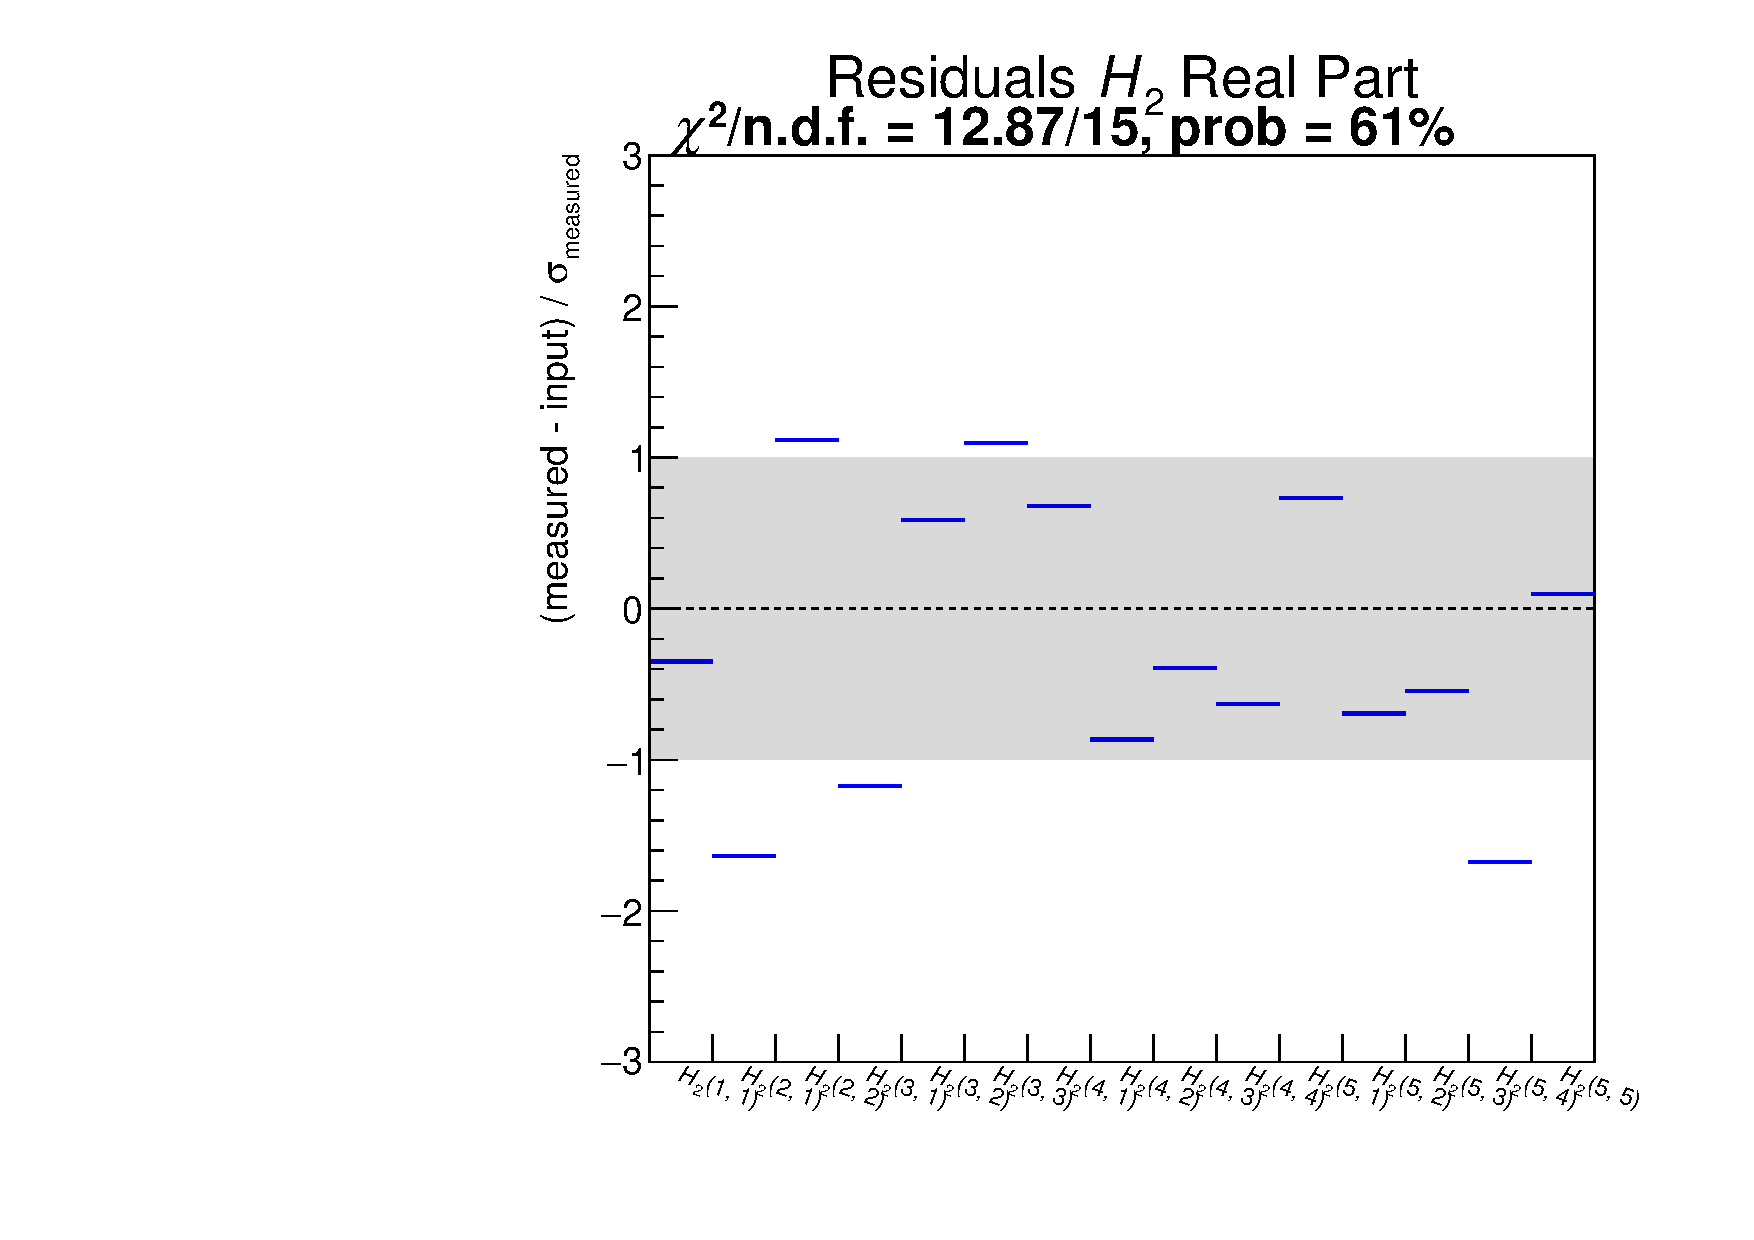
\includegraphics[width=0.5\textwidth]{photoprod/acc_1/hResiduals_H2_Re}%
  }%
  \subfloat[][]{%
    \label{fig:photoprod_study_residual_H2_im}%
    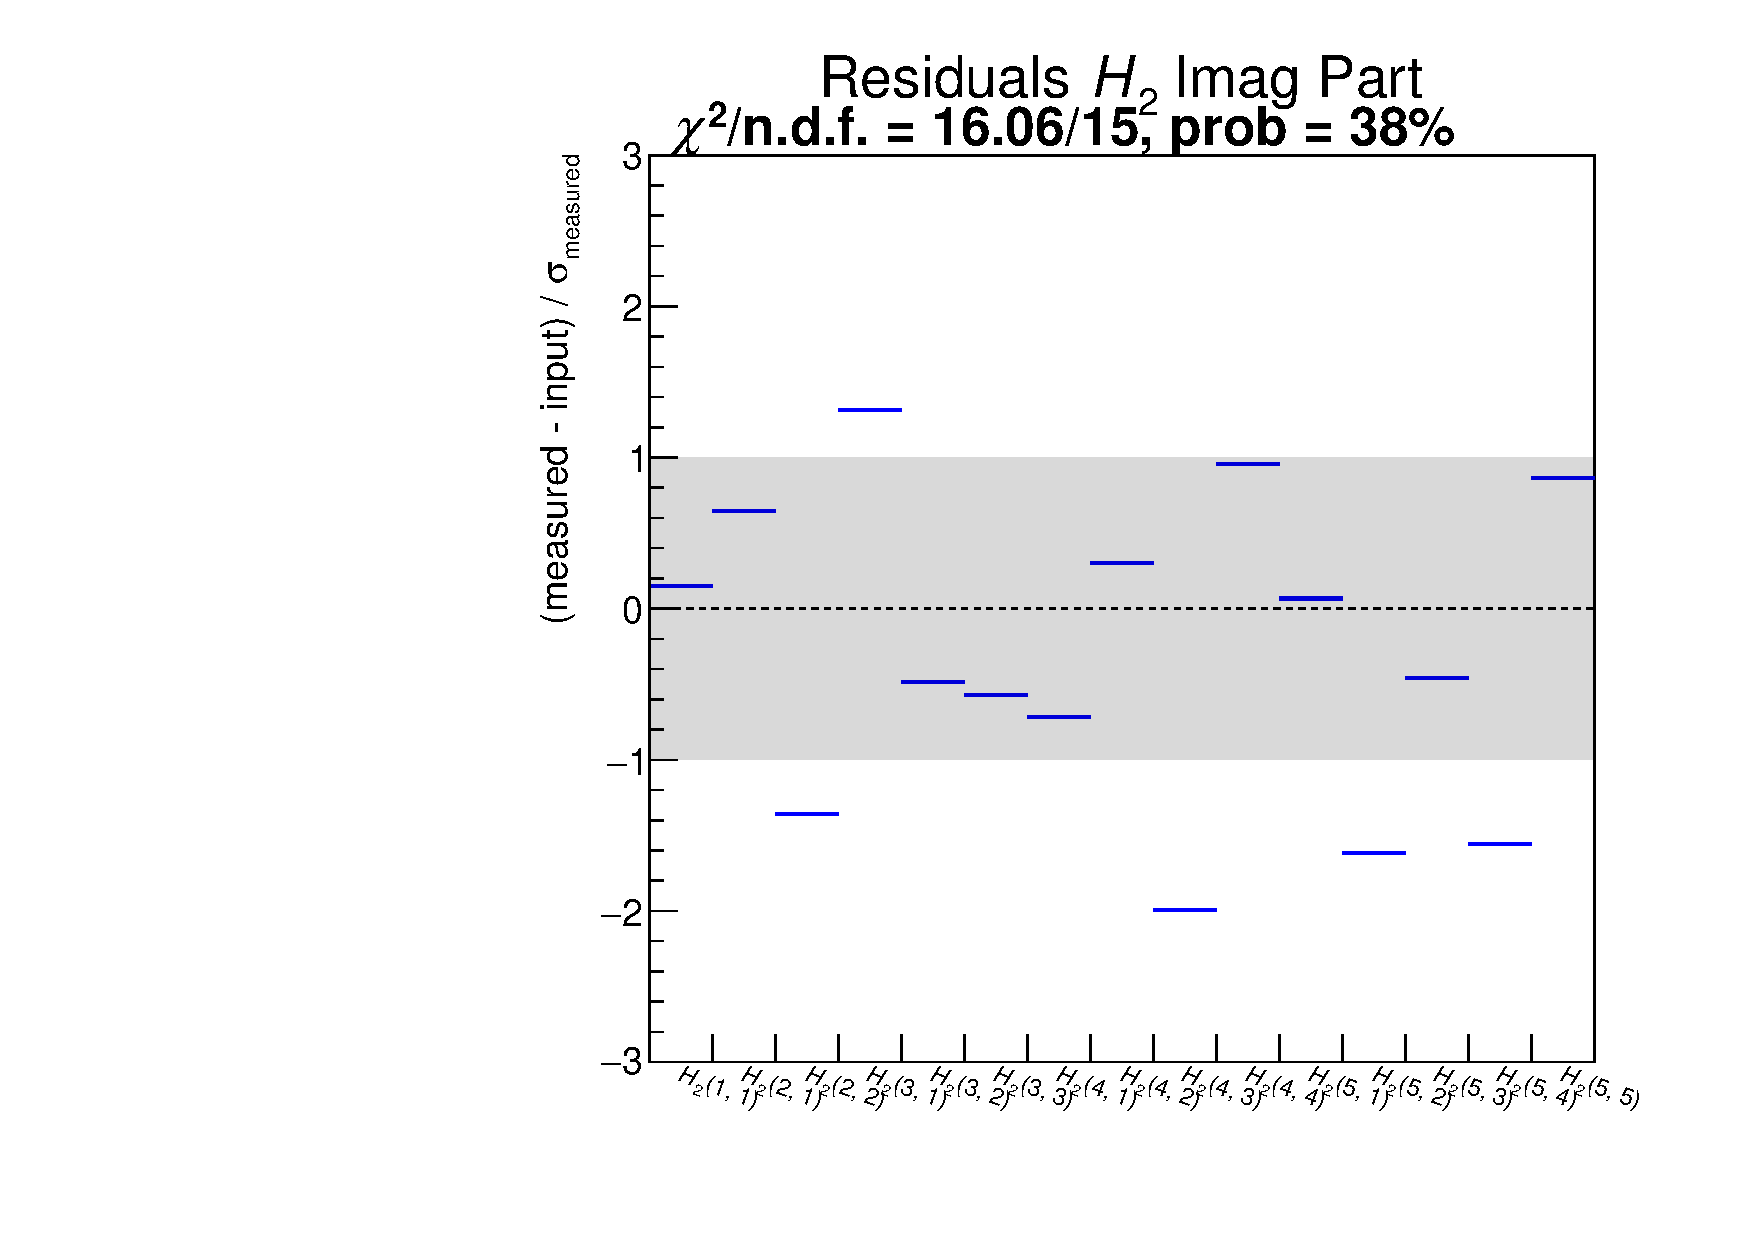
\includegraphics[width=0.5\textwidth]{photoprod/acc_1/hResiduals_H2_Im}%
  }%
  \caption{Same as \cref{fig:photoprod_study_output_H0} but for
  $H_2(L, M)$.}%
  \label{fig:photoprod_study_output_H2}%
\end{figure}


\clearpage
\subsubsection{Weighted events}%
\label{sec:photoprod:example_weighted}

To test the case of weighted events, we perform a Monte Carlo
input-output study where the physical intensity distribution is given
by the sum of a signal and a background contribution, which both have
different angular distributions.  The angular distribution of the
signal is defined by the same partial-wave amplitudes already used in
\cref{sec:photoprod:example_unweighted} (see
\cref{tab:photoprod_study_waveset}).  For the angular distribution of
the background component, we use the same set of waves, but different
amplitude values, which are listed in
\cref{tab:photoprod_study_waveset_bkg}.  In both cases, we again
assume ideal beam-photon polarization, \ie $P_\gamma = 1$.  The two
angular distributions of the intensity components are shown in
\cref{fig:photoprod_study_weighted_intensity_sig,fig:photoprod_study_weighted_intensity_bkg}.

\begin{table}[tbp]
  \centering%
  \renewcommand{\arraystretch}{1.2}%
  \caption{Partial-wave amplitude values used to generate pseudodata
  for the background component.  The wave notation is
  $\ell_m^{(\refl)}$.}%
  \label{tab:photoprod_study_waveset_bkg}%
  \vspace*{1ex}%
  \hfill%
  \begin{tabular}{ll}
    \toprule
    \textbf{Partial wave} &
    \textbf{Amplitude value} \\
    \midrule
    % negative-reflectivity waves
    $S_0^{(-)}$    & $\hphantom{-}1.0$ \\
    $P_{-1}^{(-)}$ & $-0.9 + 0.7 \imag$ \\
    $P_0^{(-)}$    & $-0.6 + 0.4 \imag$ \\
    $P_{+1}^{(-)}$ & $-0.9 - 0.8 \imag$ \\
    $D_{-2}^{(-)}$ & $-1.0 - 0.7 \imag$ \\
    $D_{-1}^{(-)}$ & $-0.8 - 0.7 \imag$ \\
    $D_0^{(-)}$    & $\hphantom{-}0.4 + 0.3 \imag$ \\
    $D_{+1}^{(-)}$ & $-0.6 - 0.1 \imag$ \\
    $D_{+2}^{(-)}$ & $-0.1 - 0.9 \imag$ \\
    \bottomrule
  \end{tabular}
  \hfill%
  \begin{tabular}{ll}
    \toprule
    \textbf{Partial wave} &
    \textbf{Amplitude value} \\
    \midrule
    % positive-reflectivity waves
    $S_0^{(+)}$    & $\hphantom{-}0.5$ \\
    $P_{-1}^{(+)}$ & $-1.0 + 0.8 \imag$ \\
    $P_0^{(+)}$    & $-0.2 + 0.2 \imag$ \\
    $P_{+1}^{(+)}$ & $\hphantom{-}0.0 - 0.3 \imag$ \\
    $D_{-2}^{(+)}$ & $\hphantom{-}0.7 + 0.9 \imag$ \\
    $D_{-1}^{(+)}$ & $-0.4 - 0.5 \imag$ \\
    $D_0^{(+)}$    & $-0.3 + 0.2 \imag$ \\
    $D_{+1}^{(+)}$ & $-1.0 - 0.4 \imag$ \\
    $D_{+2}^{(+)}$ & $\hphantom{-}0.5 - 0.2 \imag$ \\
    \bottomrule
  \end{tabular}
  \hfill\null%
\end{table}

\begin{figure}[tbp]
  \centering%
  \subfloat[][]{%
    \label{fig:photoprod_study_weighted_intensity_sig}%
    \includegraphics[width=0.5\textwidth]{photoprod_weighted/no_acc/intensitySig}%
  }%
  \subfloat[][]{%
    \label{fig:photoprod_study_weighted_intensity_bkg}%
    \includegraphics[width=0.5\textwidth]{photoprod_weighted/no_acc/intensityBkg}%
  }%
  \\%
  \subfloat[][]{%
    \label{fig:photoprod_study_weighted_data_10M}%
    \includegraphics[width=0.5\textwidth]{photoprod_weighted/no_acc_10M/data}%
  }%
  \subfloat[][]{%
    \label{fig:photoprod_study_weighted_discr_var_10M}%
    \includegraphics[width=0.5\textwidth]{photoprod_weighted/no_acc_10M/hDiscrVariableSim}%
  }%
  \caption{\subfloatLabel{fig:photoprod_study_weighted_intensity_sig}~Intensity
  distribution used to generate the signal component as defined by the
  partial-wave amplitudes listed in
  \cref{tab:photoprod_study_waveset}.
  \subfloatLabel{fig:photoprod_study_weighted_intensity_bkg}~Intensity
  distribution used to generate the background component as defined by
  the partial-wave amplitudes listed in
  \cref{tab:photoprod_study_waveset_bkg}.
  \subfloatLabel{fig:photoprod_study_weighted_data_10M}~Total Monte
  Carlo data sample obtained by randomly drawing \num{e7}~events from
  each of the distributions
  in~\subfloatLabel{fig:photoprod_study_weighted_intensity_sig}
  and~\subfloatLabel{fig:photoprod_study_weighted_intensity_bkg}.
  \subfloatLabel{fig:photoprod_study_weighted_discr_var_10M}~Distribution
  of the discriminatory variable for the total Monte Carlo data sample
  in~\subfloatLabel{fig:photoprod_study_weighted_data_10M}.  The
  shaded regions indicate the signal and side bands.}%
  \label{fig:photoprod_study_weighted}%
\end{figure}

The angular distributions are disentangled by applying a
one-dimensional sideband subtraction in a hypothetical discriminating
variable, which covers the range $[-1, +1]$.\footnote{In practice,
this could be, for example, the invariant mass distribution of an
unstable daughter particle.}  In this variable, the signal is
generated according to a Gaussian, which is centered at~0 and has a
standard deviation of~0.1, while the background is generated
uniformly.  The signal band in the discriminating variable is $[-0.3,
+0.3]$.  Events in this range, are assigned a weight of $w_k = +1$.
The sidebands are $[-1.0, -0.4]$ and $[+0.4, +1.0]$.  Events in these
ranges are assigned a weight of $w_k = -1/2$.\todo{add bands as well
as signal and background components to
\cref{fig:photoprod_study_weighted_discr_var_10M}}

To verify that the sideband subtraction works, we generate a random
data sample containing \num{e7}~signal events and the same amount of
background events.  \Cref{fig:photoprod_study_weighted_data_10M} shows
the resulting angular distribution and
\cref{fig:photoprod_study_weighted_discr_var_10M}  the distribution of
the discriminatory variable.  As expected, we recover the angular
distribution of the signal component by applying the sideband
subtraction (\confer
\cref{fig:photoprod_study_weighted_data_sb_subtr_10M} with
\cref{fig:photoprod_study_weighted_intensity_sig}).

\begin{figure}[tbp]
  \centering%
  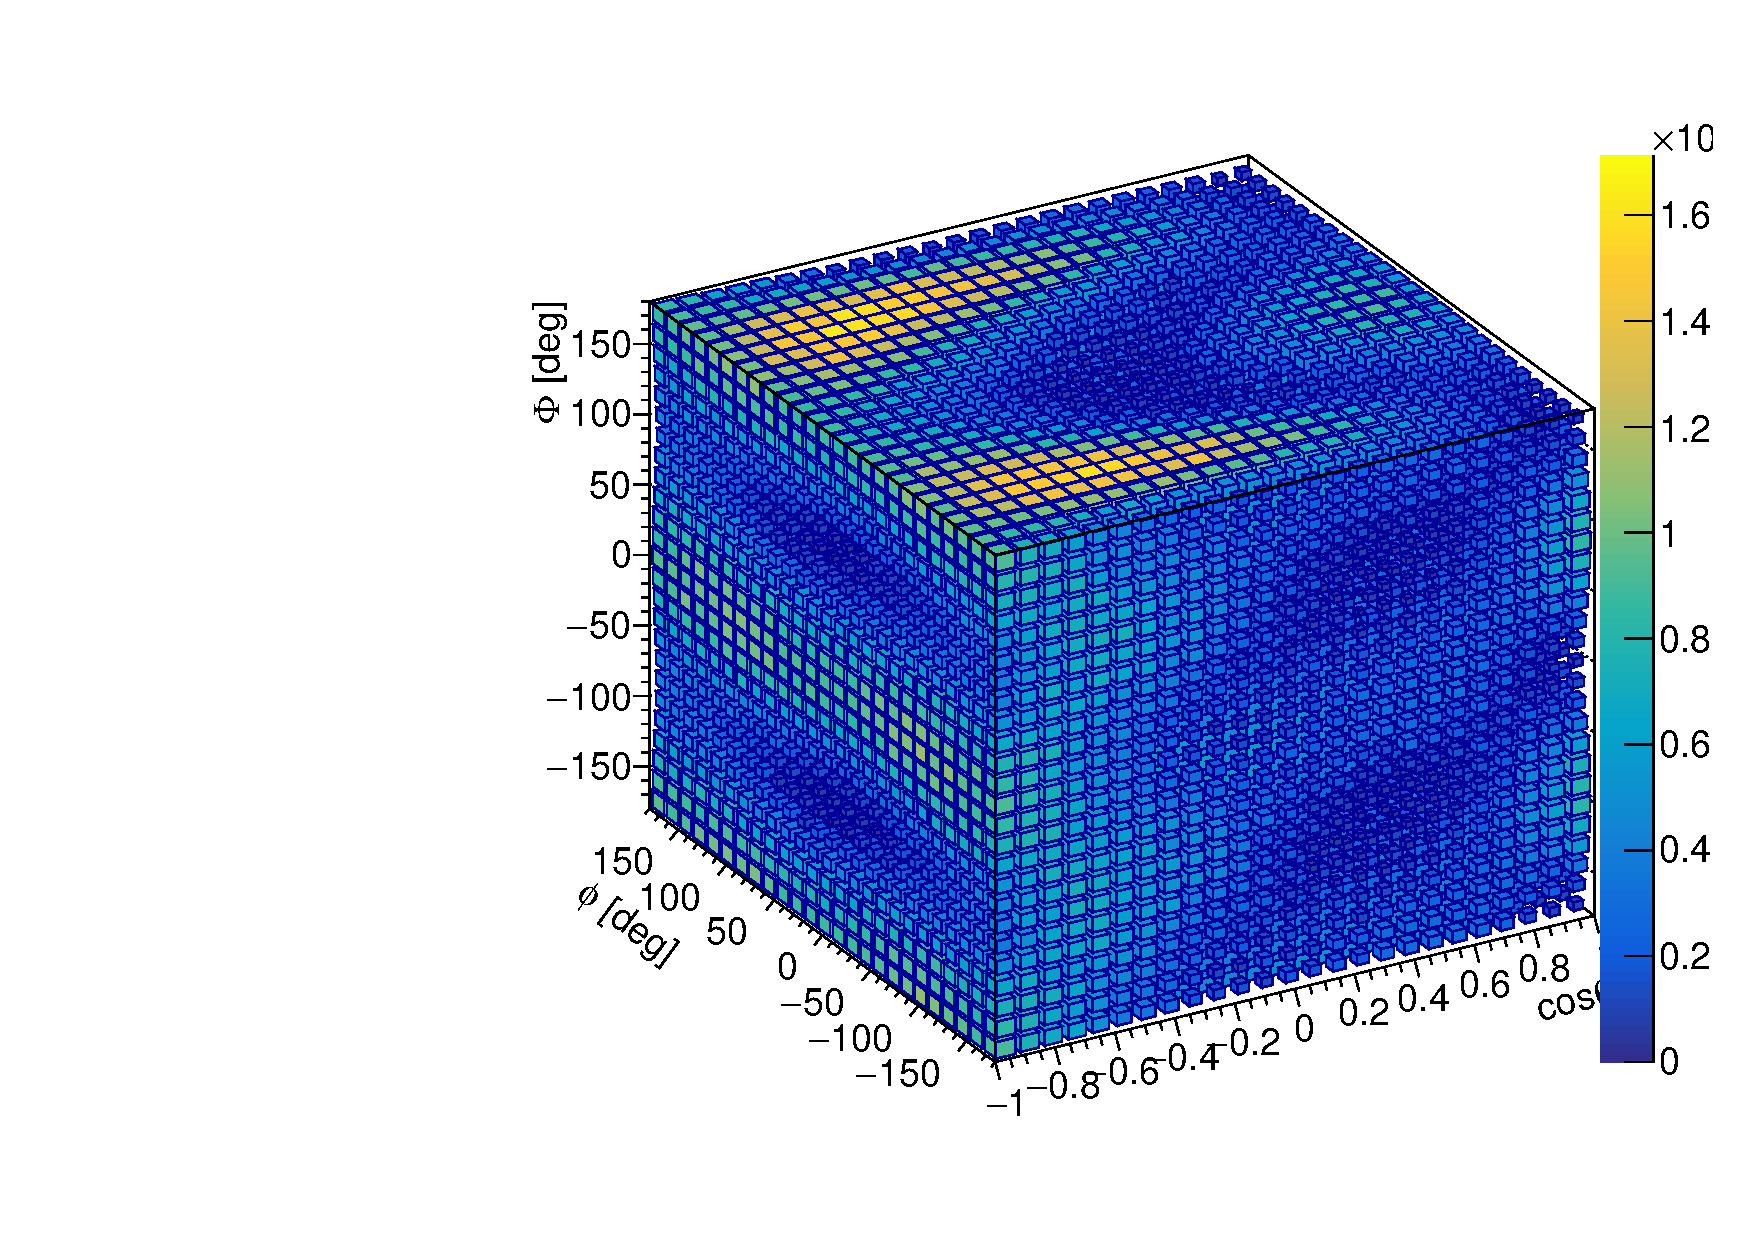
\includegraphics[width=0.5\textwidth]{photoprod_weighted/no_acc_10M/dataSbSubtr}%
  \caption{Signal sample with $N_\text{sig} = \num{9974322.5}$ signal
  events obtained from \cref{fig:photoprod_study_weighted_data_10M} by
  applying sideband subtraction using the discriminatory variable in
  \cref{fig:photoprod_study_weighted_discr_var_10M}.  Compare to
  \cref{fig:photoprod_study_weighted_intensity_sig}.}%
  \label{fig:photoprod_study_weighted_data_sb_subtr_10M}%
\end{figure}

For the moment analysis, we weight the intensity distributions of the
signal and the background component with the hypothetical detection
efficiency in \cref{eq:photoprod_study_acc1}, which is shown in
\cref{fig:photoprod_study_efficiency}.  From each of these weighted
intensity distributions (see
\cref{fig:photoprod_study_weighted_intensity_sig_acc,fig:photoprod_study_weighted_intensity_bkg_acc}),
we randomly draw a sample of \num{1000}~events.  The distribution of
the total sample in the discriminatory variable is shown in
\cref{fig:photoprod_study_weighted_discr_var}, the corresponding
angular distribution in \cref{fig:photoprod_study_weighted_data}.  The
sample is used to calculate the values of the measured
moments~$\hat{\vect{H}}_\text{meas}$ using
\cref{eq:photoprod_moments_meas_estimate_weighted} as well as their
augmented covariance matrix using the approach described in
\cref{fn:cov_aug_numpy}.

\begin{figure}[tbp]
  \centering%
  \subfloat[][]{%
    \label{fig:photoprod_study_weighted_intensity_sig_acc}%
    \includegraphics[width=0.5\textwidth]{photoprod_weighted/acc_1/intensitySig}%
  }%
  \subfloat[][]{%
    \label{fig:photoprod_study_weighted_intensity_bkg_acc}%
    \includegraphics[width=0.5\textwidth]{photoprod_weighted/acc_1/intensityBkg}%
  }%
  \\%
  \subfloat[][]{%
    \label{fig:photoprod_study_weighted_data}%
    \includegraphics[width=0.5\textwidth]{photoprod_weighted/acc_1/data}%
  }%
  \subfloat[][]{%
    \label{fig:photoprod_study_weighted_discr_var}%
    \includegraphics[width=0.5\textwidth]{photoprod_weighted/acc_1/hDiscrVariableSim}%
  }%
  \caption{\subfloatLabel{fig:photoprod_study_weighted_intensity_sig}~Intensity
  distribution used to generate the signal component as defined by the
  partial-wave amplitudes listed in
  \cref{tab:photoprod_study_waveset}.
  \subfloatLabel{fig:photoprod_study_weighted_intensity_bkg}~Intensity
  distribution used to generate the background component as defined by
  the partial-wave amplitudes listed in
  \cref{tab:photoprod_study_waveset_bkg}.
  \subfloatLabel{fig:photoprod_study_weighted_data_10M}~Total Monte
  Carlo data sample obtained by randomly drawing \num{e3}~events from
  each of the distributions
  in~\subfloatLabel{fig:photoprod_study_weighted_intensity_sig}
  and~\subfloatLabel{fig:photoprod_study_weighted_intensity_bkg}.
  \subfloatLabel{fig:photoprod_study_weighted_discr_var}~Distribution
  of the discriminatory variable for the total Monte Carlo data sample
  in~\subfloatLabel{fig:photoprod_study_weighted_data_10M}.  The
  shaded regions indicate the signal and side bands.}%
  \label{fig:photoprod_study_weighted_input}%
\end{figure}

Since the detection efficiency is the same as in the unweighted case,
we use the same acceptance integral matrix as in
\cref{sec:photoprod:example_unweighted} to calculate the physical
moments.
\Crefrange{fig:photoprod_study_weighted_output_H0}{fig:photoprod_study_weighted_output_H2}
show the physical moments of the signal component extracted from the
Monte Carlo data in \cref{fig:photoprod_study_weighted_data} and
compare them to the expected moment values calculated from the
partial-wave amplitudes in \cref{tab:photoprod_study_waveset} using
\crefrange{eq:photoprod_moment_0_pw_refl}{eq:photoprod_moment_2_pw_refl}.
As expected, the two sets of values  agree within statistical
uncertainties (see
\cref{fig:photoprod_study_weighted_residual_H0_re,fig:photoprod_study_weighted_residual_H1_re,fig:photoprod_study_weighted_residual_H2_im}).
Since the $H_0(L, M)$ and $H_1(L, M)$ are expected to be real-valued
and $H_2(L, M)$ to be purely imaginary (see
\cref{eq:photoprodP_moments_real_imag}), we also verify that the
imaginary parts of $H_{0, 1}(L, M)$ and the real parts of $H_2(L, M)$
are consistent with zero, which is indeed the case (see
\cref{fig:photoprod_study_weighted_comparison_H0_im,fig:photoprod_study_weighted_residual_H0_im,fig:photoprod_study_weighted_comparison_H1_im,fig:photoprod_study_weighted_residual_H1_im,fig:photoprod_study_weighted_comparison_H2_re,fig:photoprod_study_weighted_residual_H2_re}).

\begin{figure}[tbp]
  \centering%
  \subfloat[][]{%
    \label{fig:photoprod_study_weighted_comparison_H0_re}%
    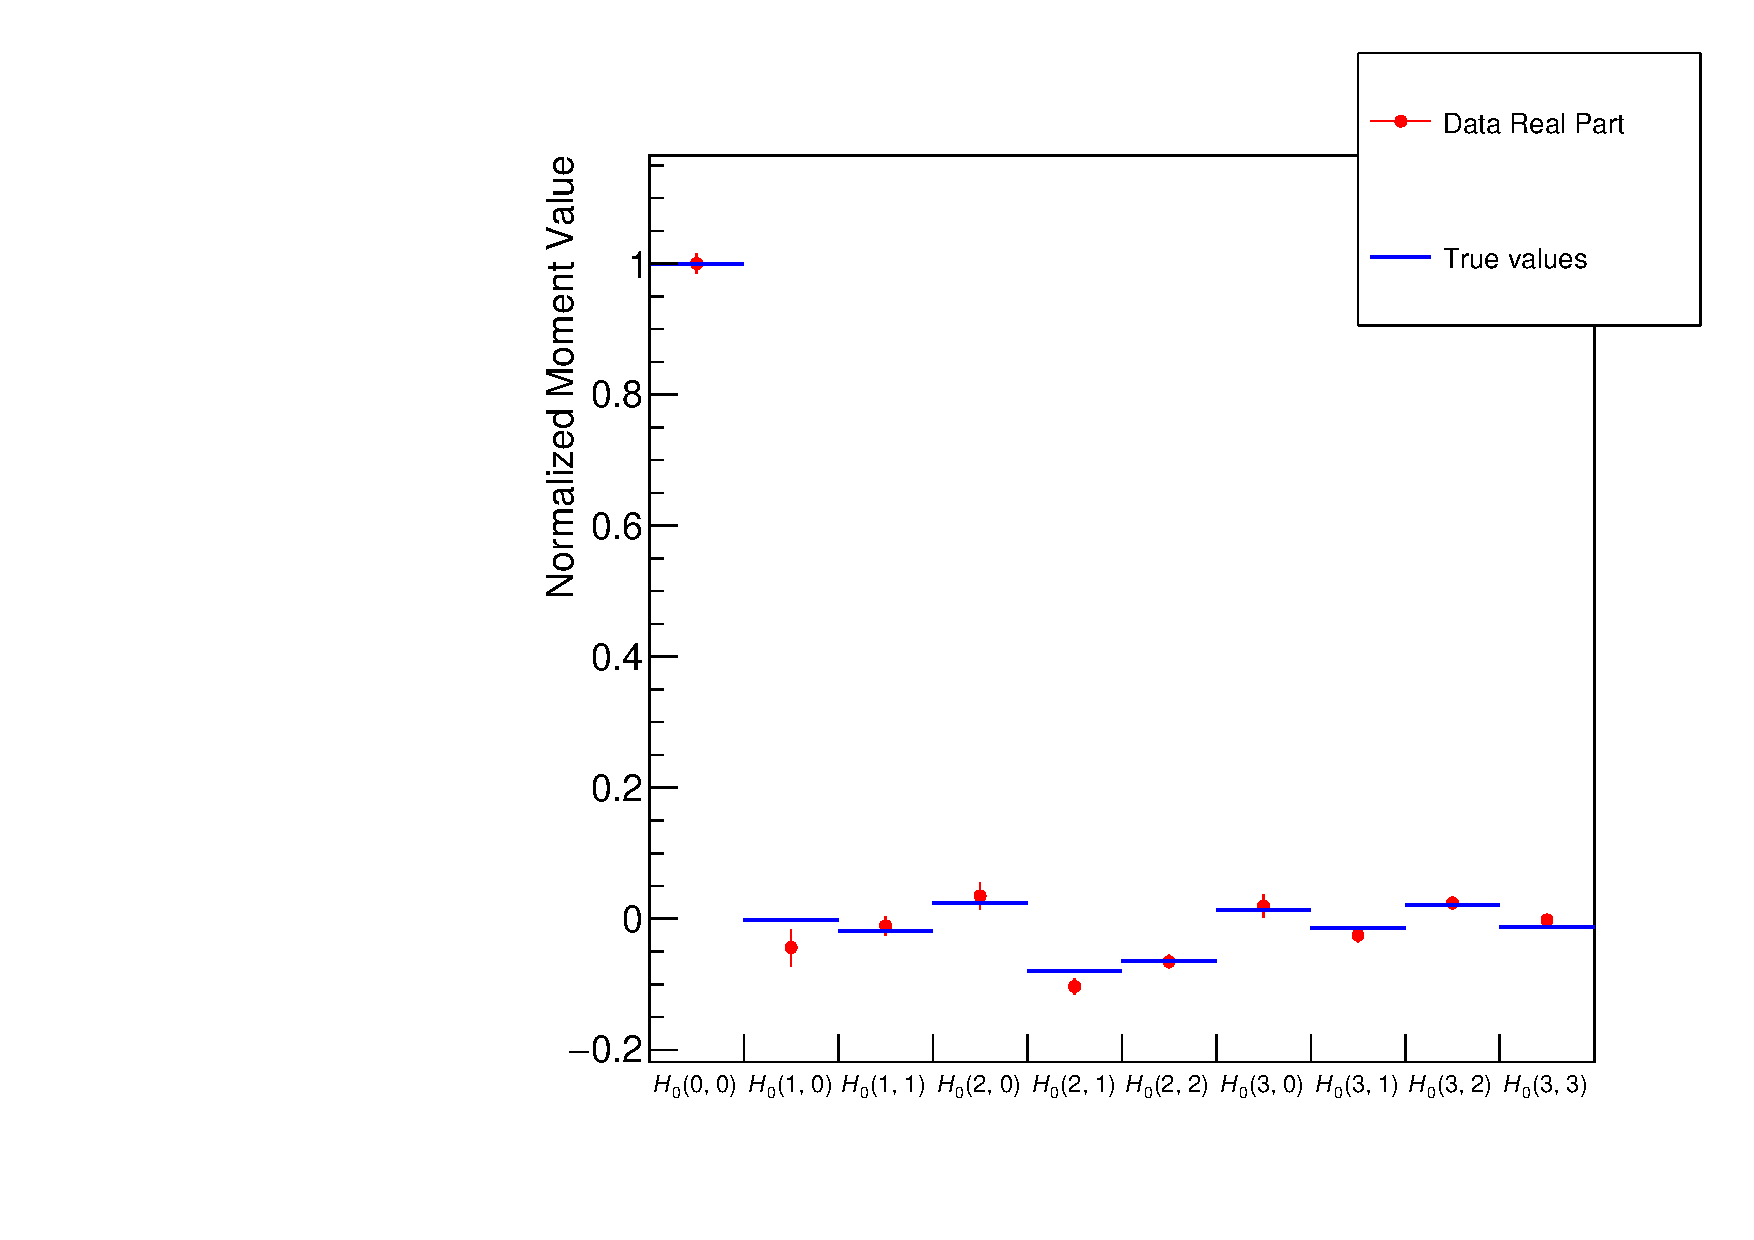
\includegraphics[width=0.5\textwidth]{photoprod_weighted/acc_1/hmass_1.50_Compare_H0_Re}%
  }%
  \subfloat[][]{%
    \label{fig:photoprod_study_weighted_comparison_H0_im}%
    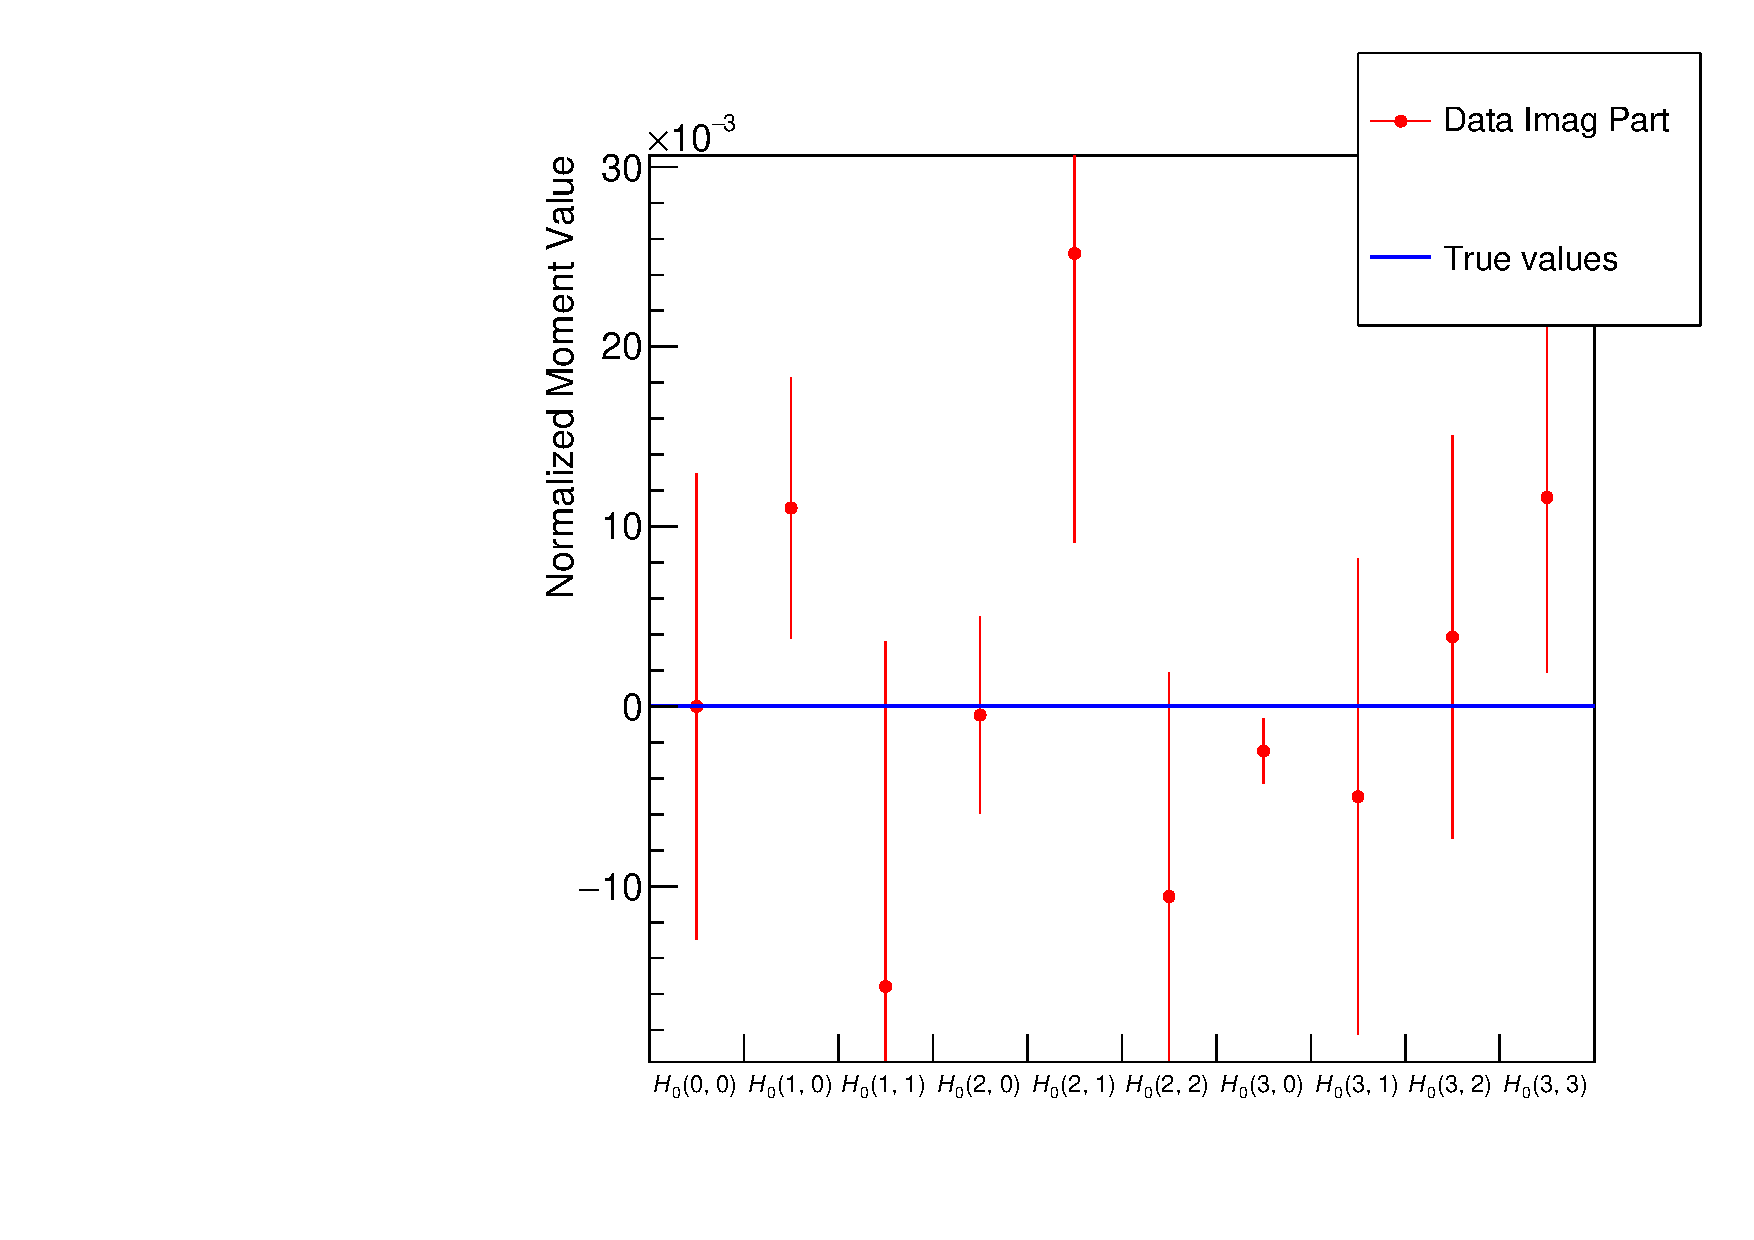
\includegraphics[width=0.5\textwidth]{photoprod_weighted/acc_1/hmass_1.50_Compare_H0_Im}%
  }%
  \\%
  \subfloat[][]{%
    \label{fig:photoprod_study_weighted_residual_H0_re}%
    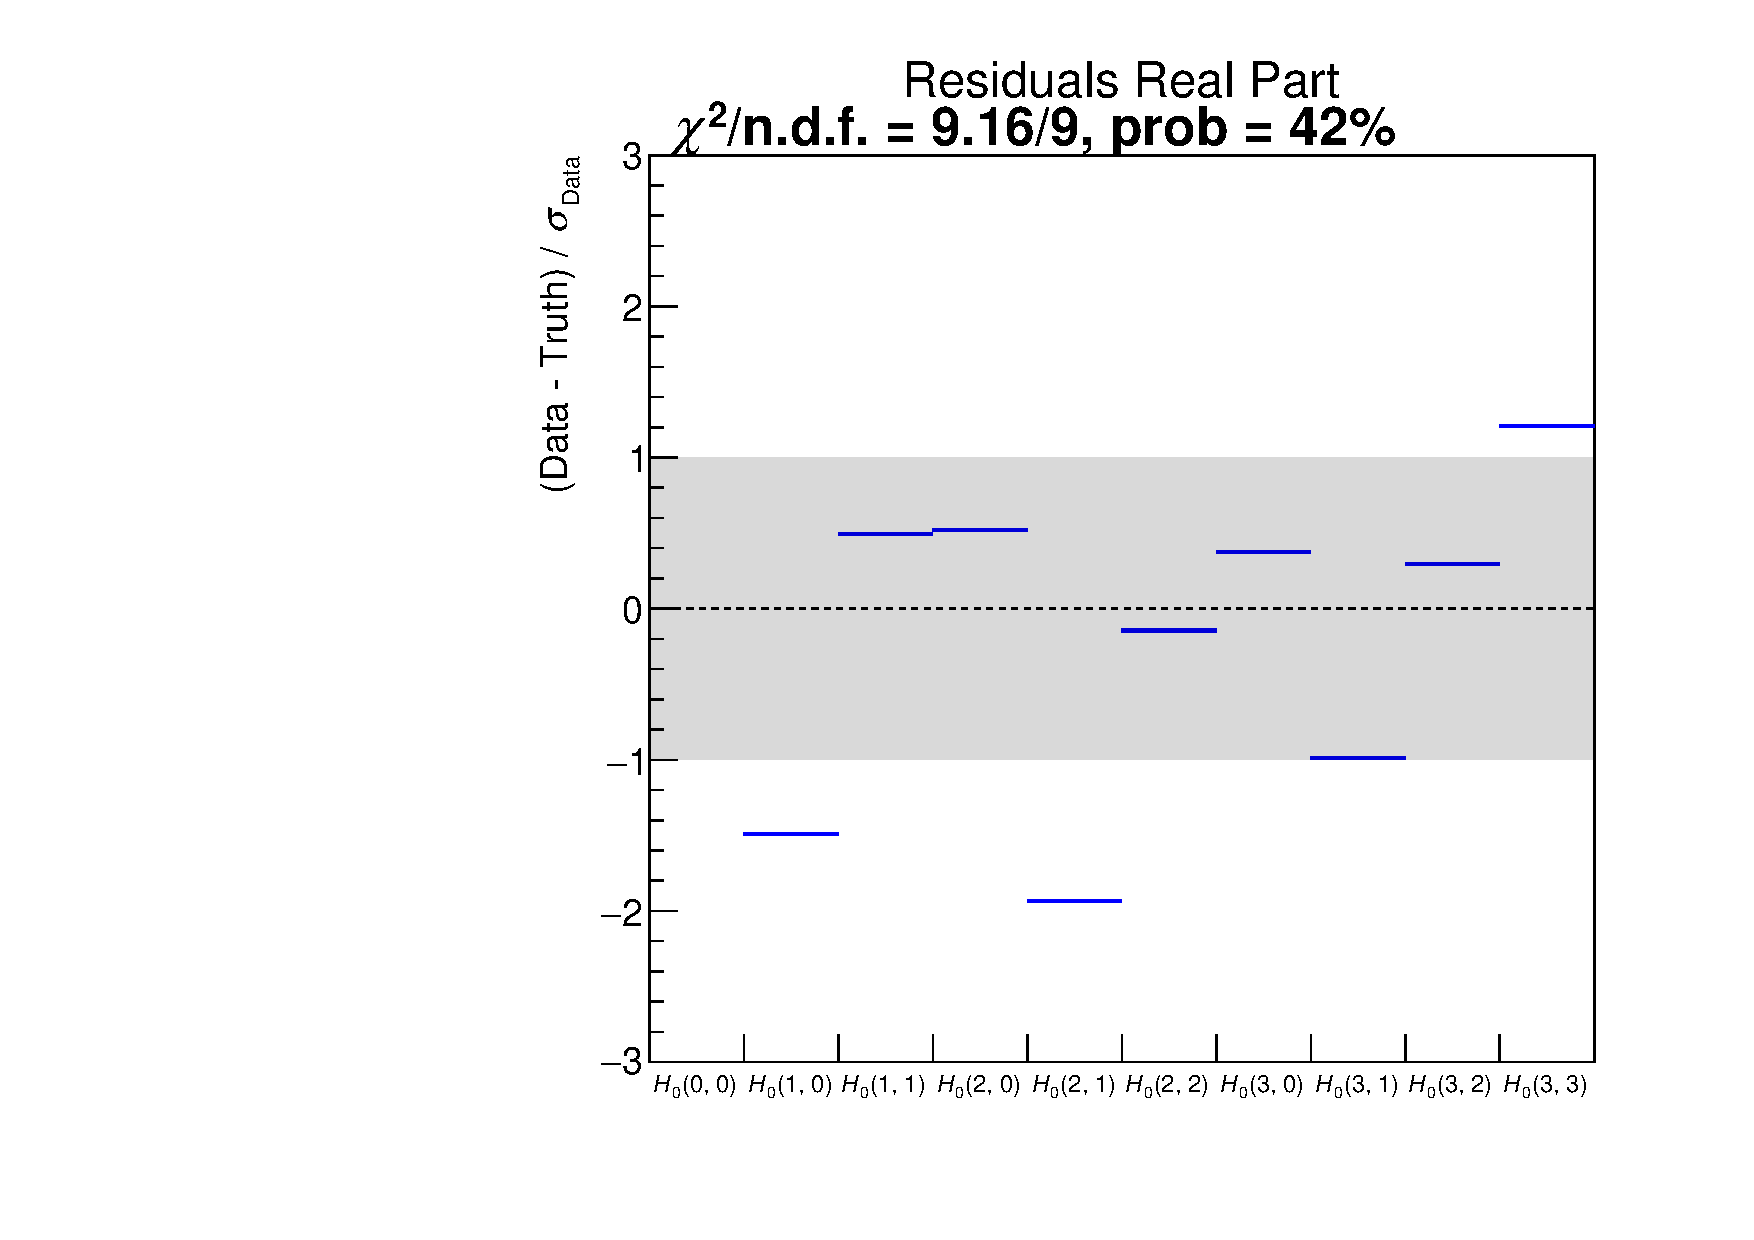
\includegraphics[width=0.5\textwidth]{photoprod_weighted/acc_1/hmass_1.50_Residuals_H0_Re}%
  }%
  \subfloat[][]{%
    \label{fig:photoprod_study_weighted_residual_H0_im}%
    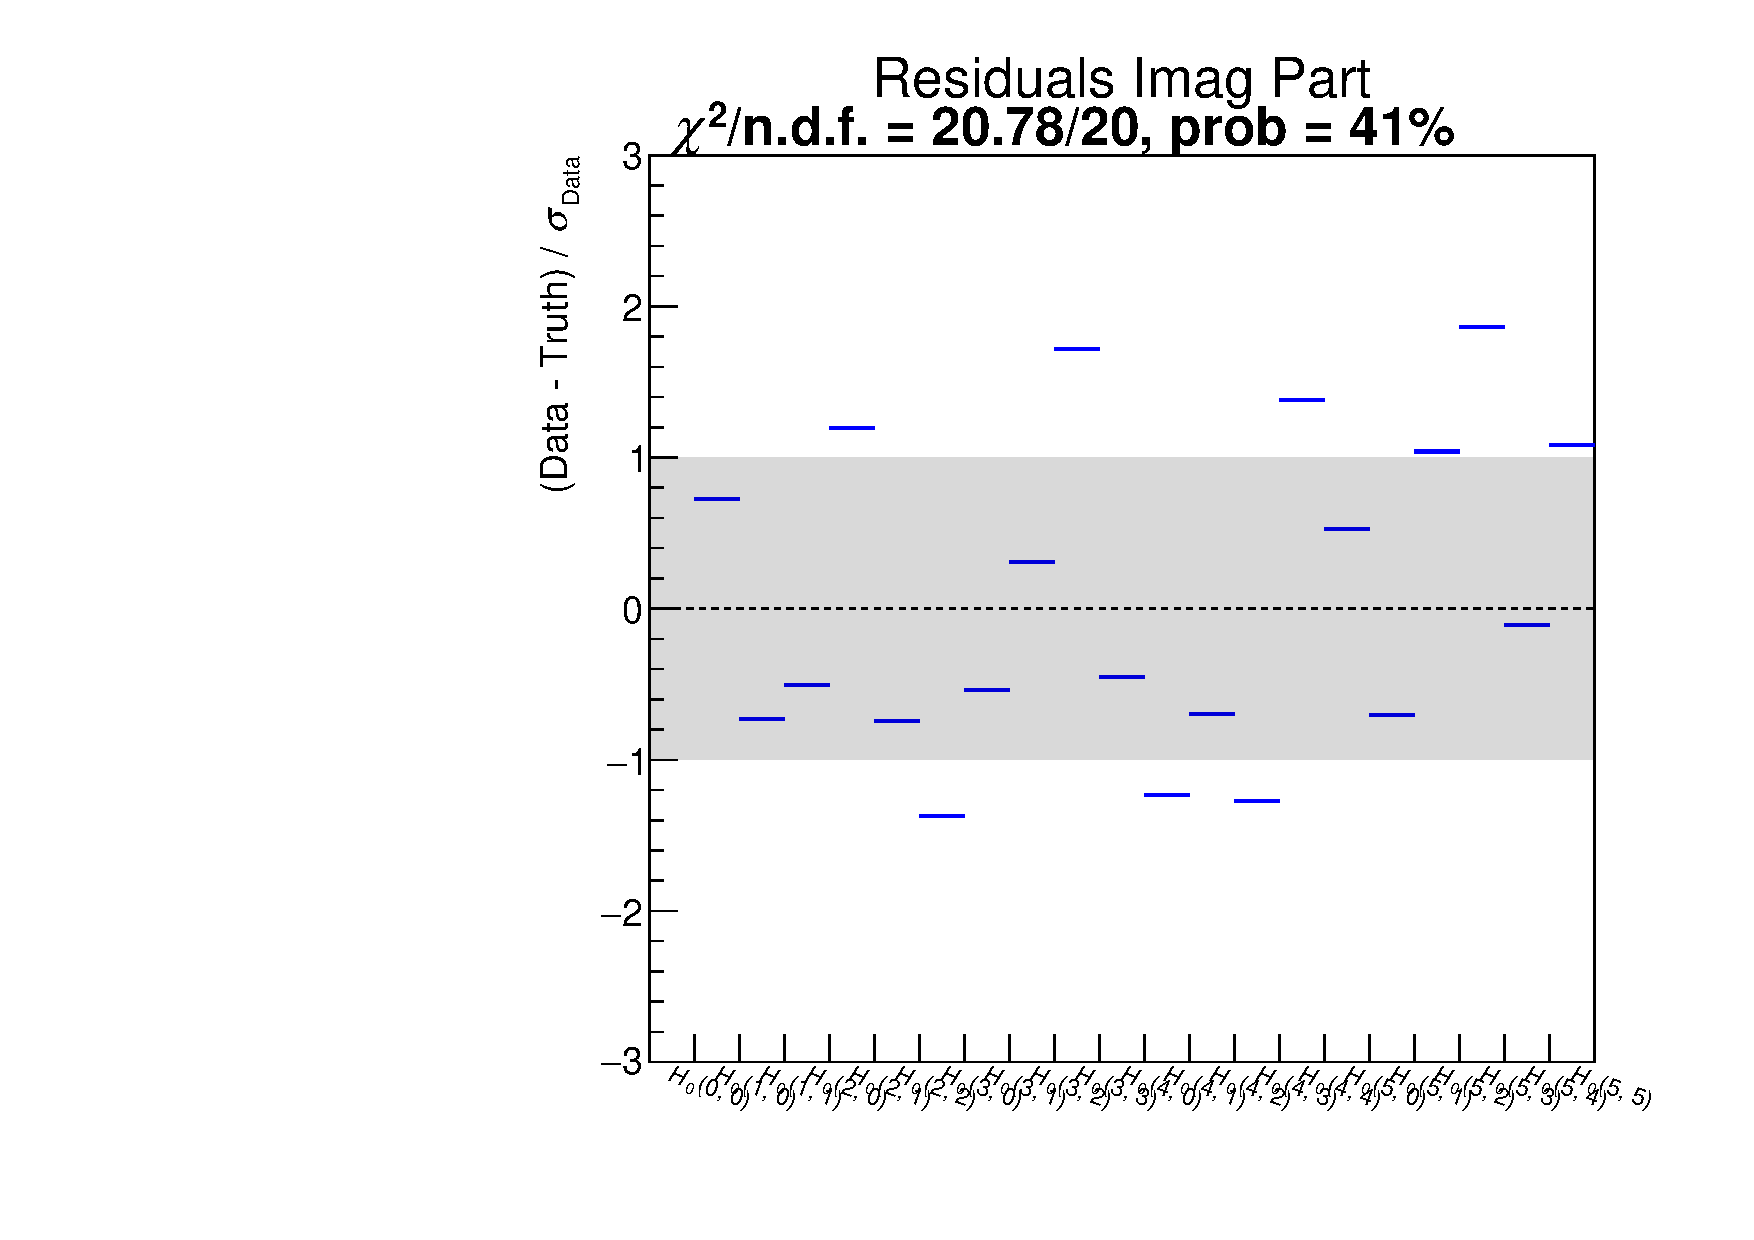
\includegraphics[width=0.5\textwidth]{photoprod_weighted/acc_1/hmass_1.50_Residuals_H0_Im}%
  }%
  \caption{Upper row: Comparison of the physical moments $H_0(L, M)$
  (red points with uncertainties) extracted from the
  sideband-subtracted Monte Carlo data, which are generated using the
  partial-wave amplitudes in
  \cref{tab:photoprod_study_waveset,tab:photoprod_study_waveset_bkg}
  and the detection efficiency in \cref{eq:photoprod_study_acc1}, with
  the expected values (blue lines).  Both sets of values are
  normalized to the value of $H_0(0, 0)$ in the respective set.
  \subfloatLabel{fig:photoprod_study_comparison_H0_re}~shows the real
  part of $H_0(L, M)$,
  \subfloatLabel{fig:photoprod_study_comparison_H0_im}~the imaginary
  part.  Note that moments with $L > 4$ are expected to be zero due to
  the chosen wave set.  Lower row: corresponding residuals.}%
  \label{fig:photoprod_study_weighted_output_H0}%
\end{figure}

\begin{figure}[tbp]
  \centering%
  \subfloat[][]{%
    \label{fig:photoprod_study_weighted_comparison_H1_re}%
    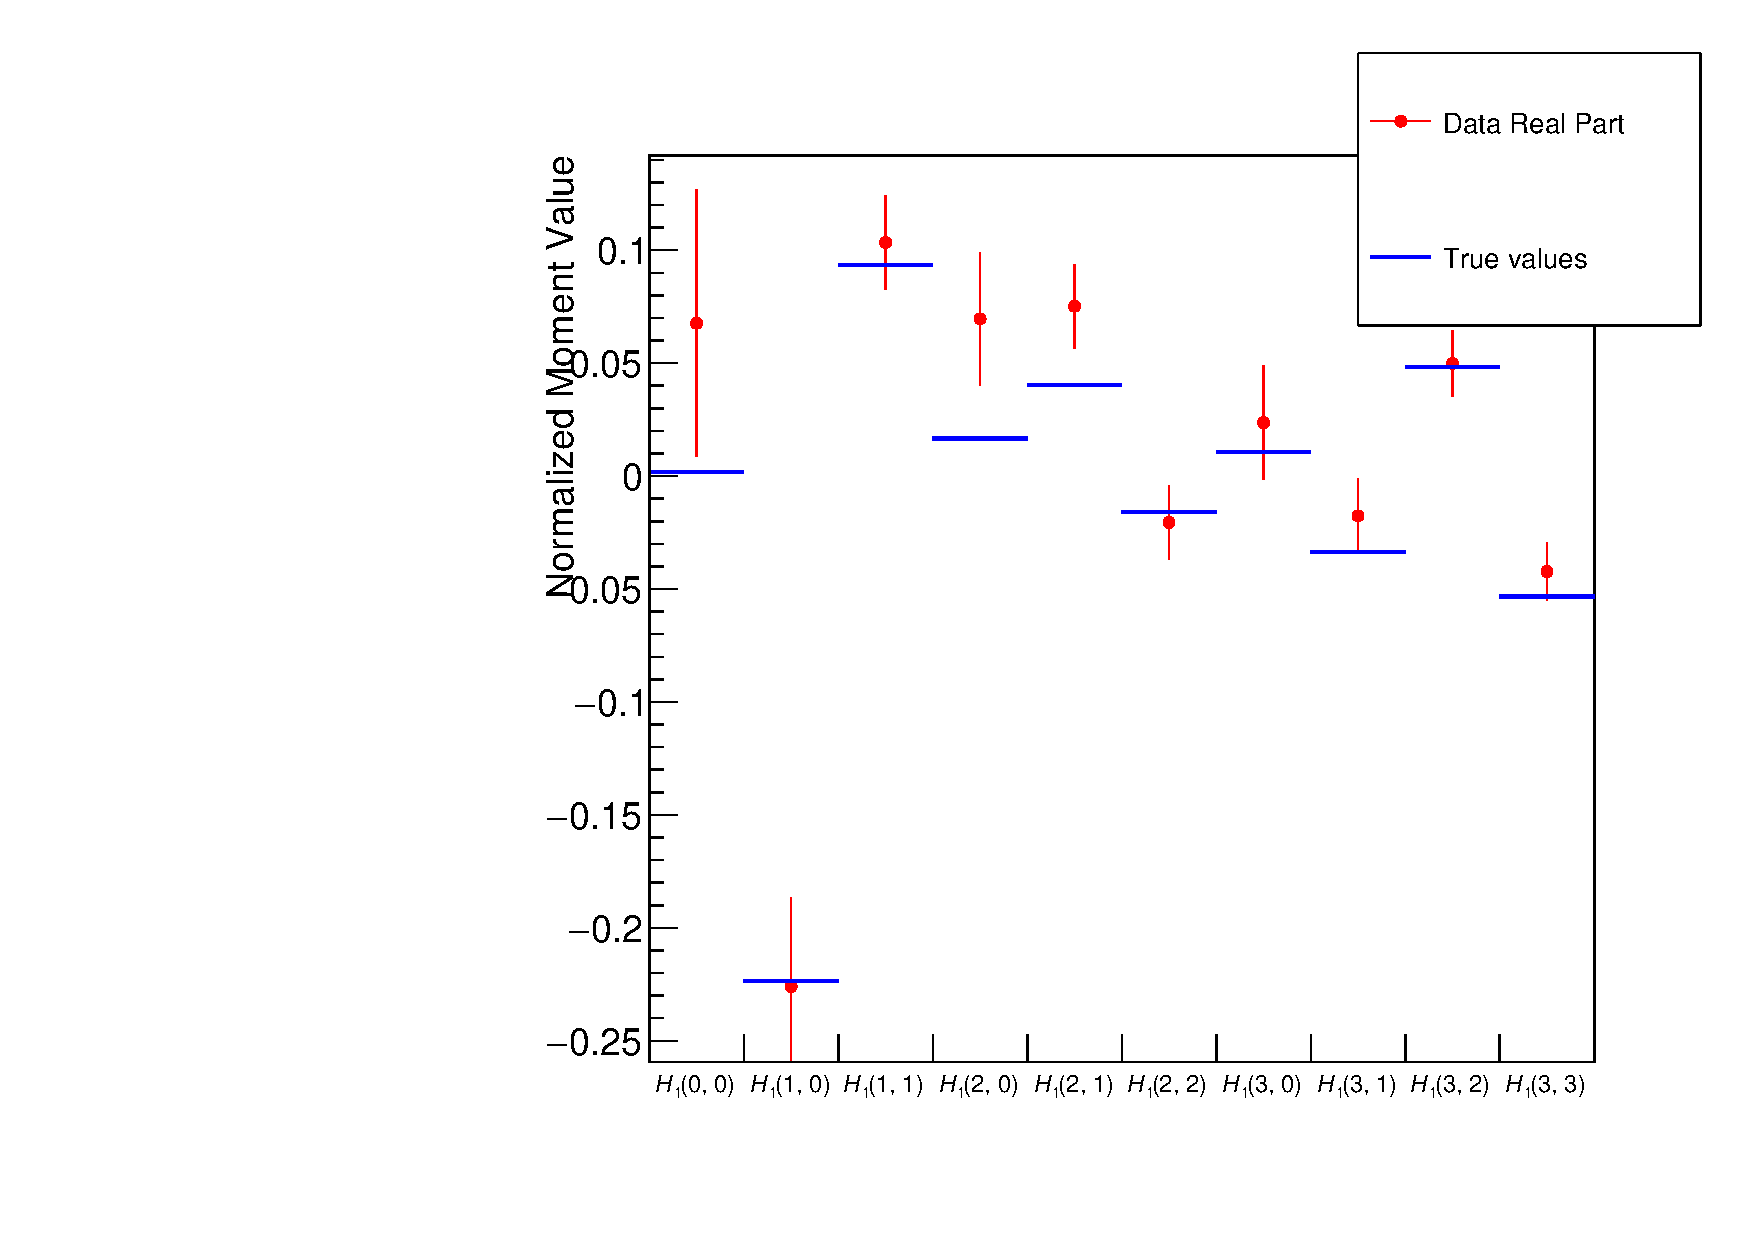
\includegraphics[width=0.5\textwidth]{photoprod_weighted/acc_1/hmass_1.50_Compare_H1_Re}%
  }%
  \subfloat[][]{%
    \label{fig:photoprod_study_weighted_comparison_H1_im}%
    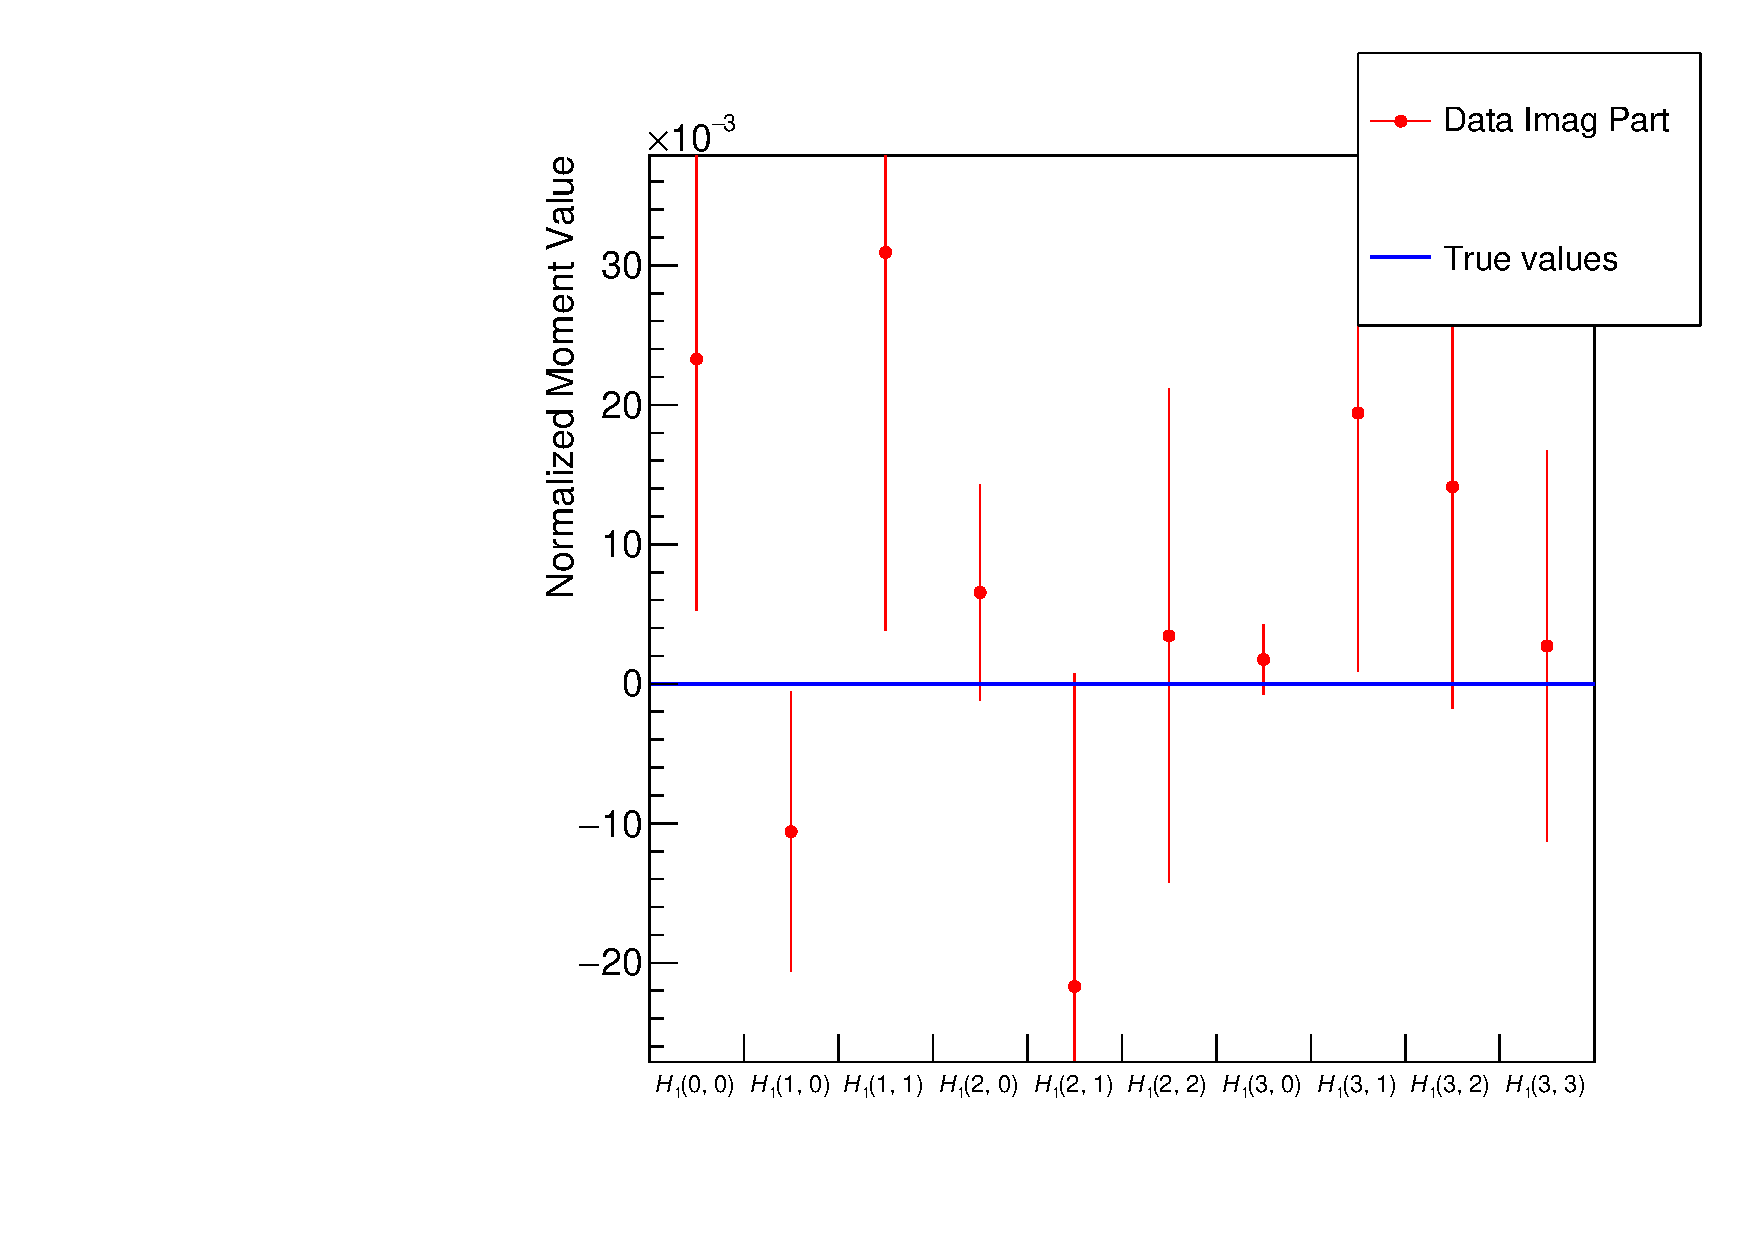
\includegraphics[width=0.5\textwidth]{photoprod_weighted/acc_1/hmass_1.50_Compare_H1_Im}%
  }%
  \\%
  \subfloat[][]{%
    \label{fig:photoprod_study_weighted_residual_H1_re}%
    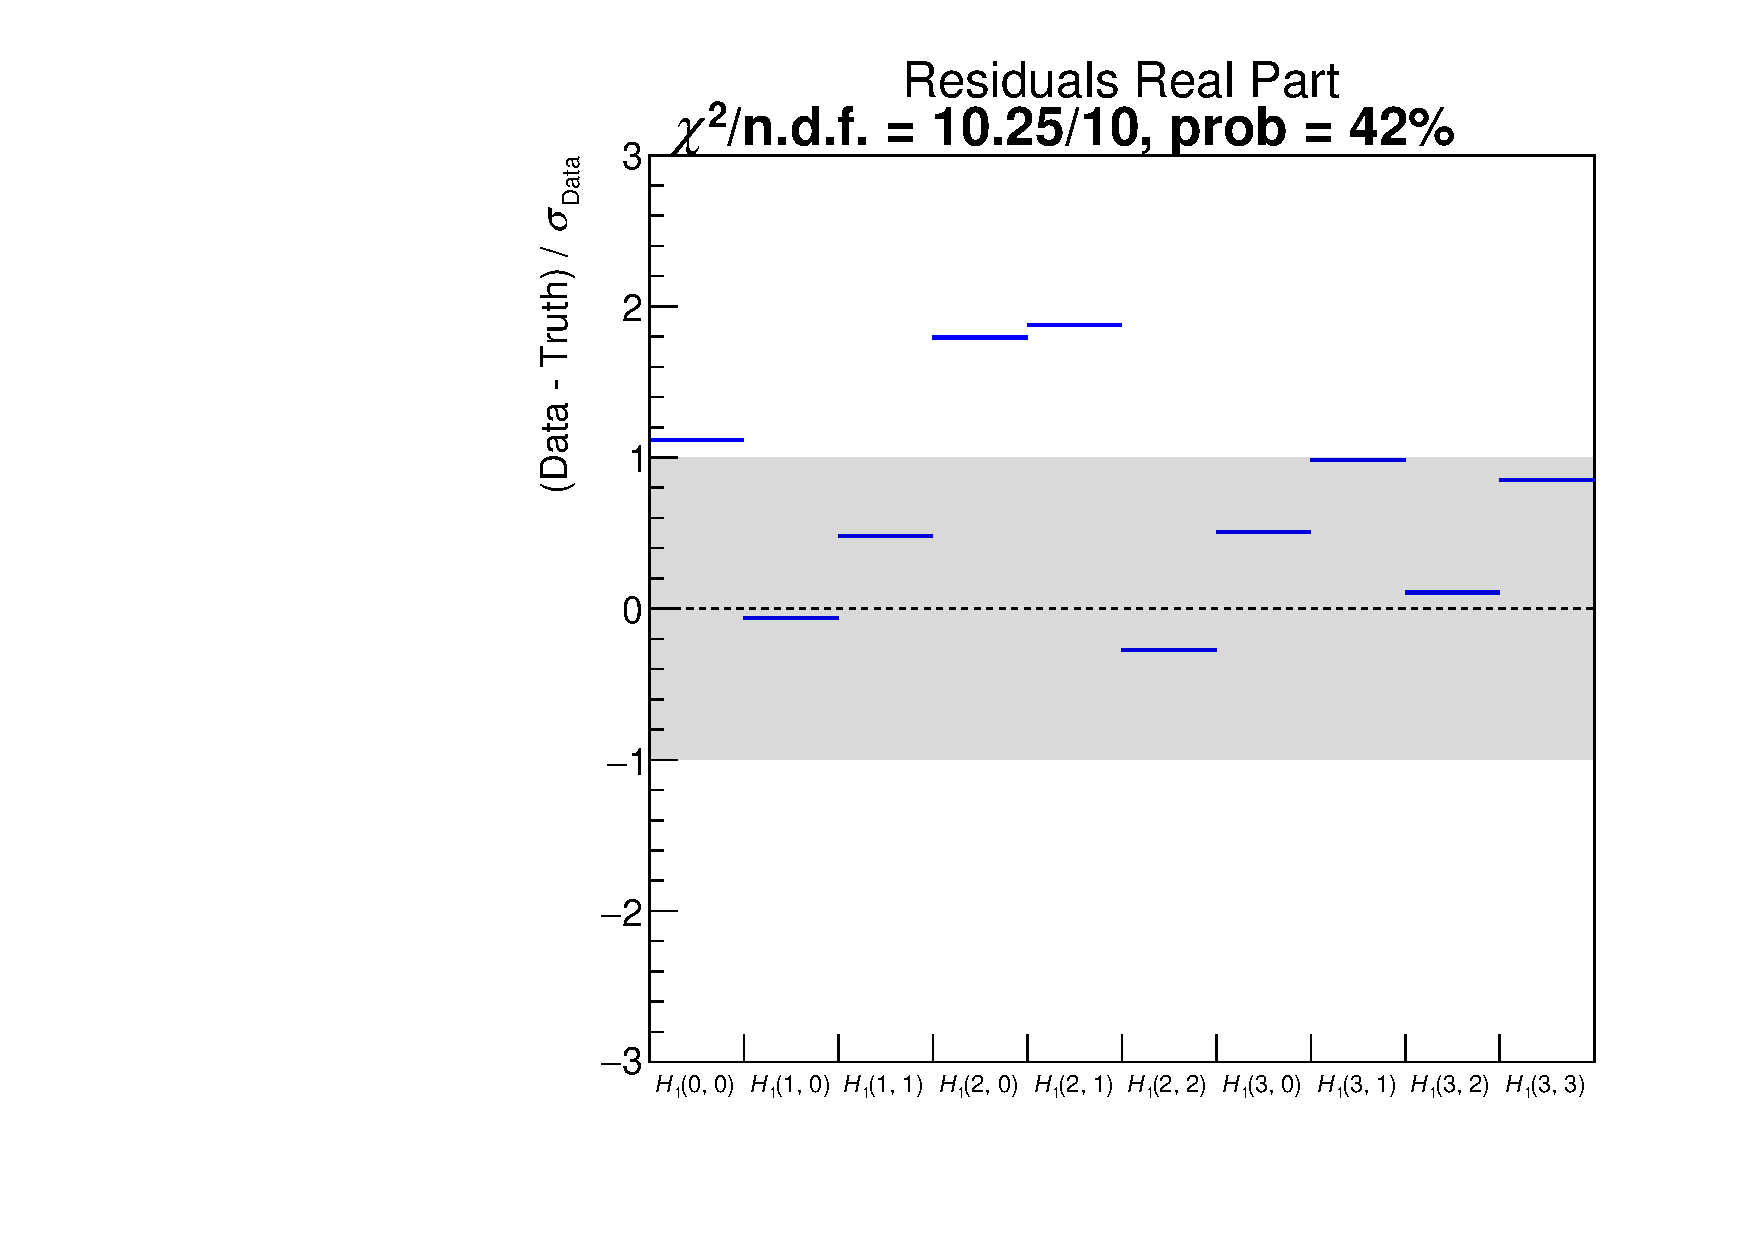
\includegraphics[width=0.5\textwidth]{photoprod_weighted/acc_1/hmass_1.50_Residuals_H1_Re}%
  }%
  \subfloat[][]{%
    \label{fig:photoprod_study_weighted_residual_H1_im}%
    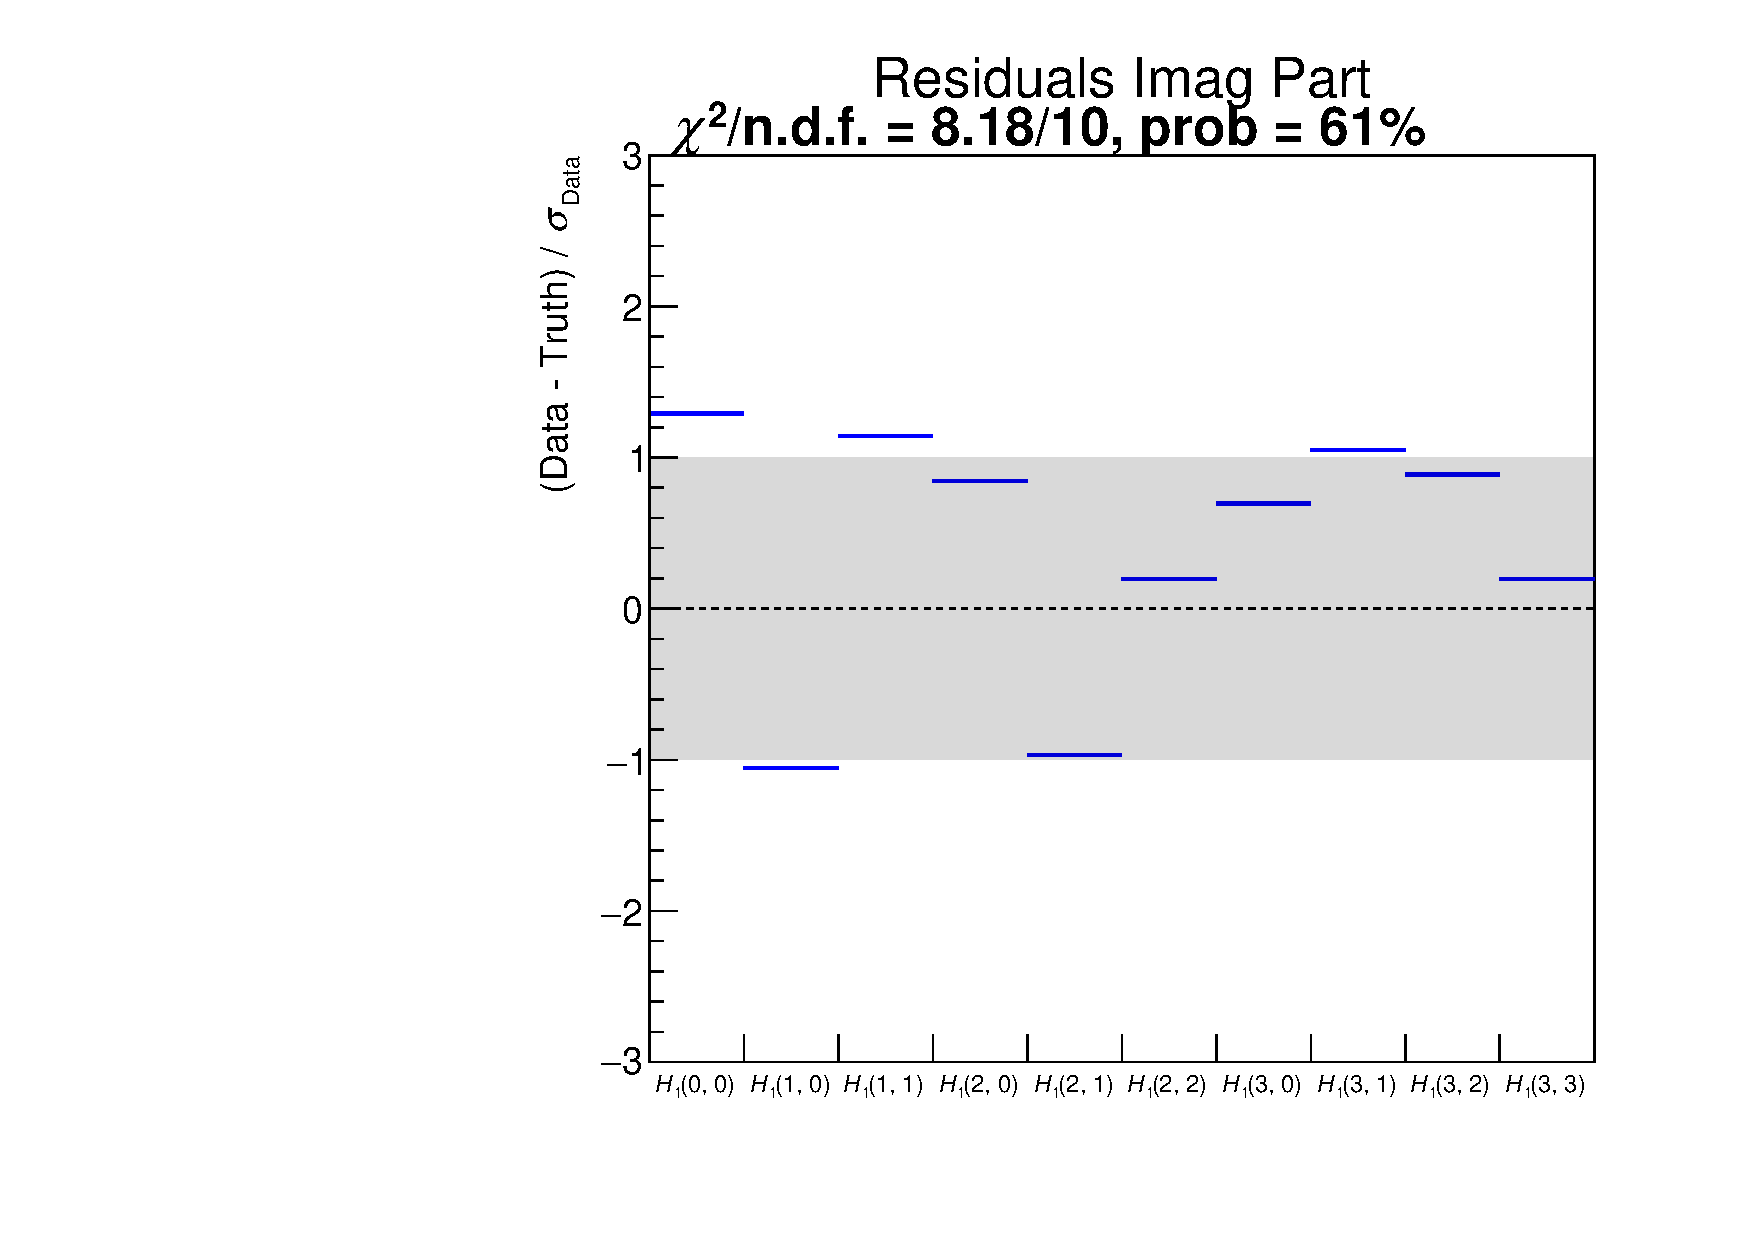
\includegraphics[width=0.5\textwidth]{photoprod_weighted/acc_1/hmass_1.50_Residuals_H1_Im}%
  }%
  \caption{Same as \cref{fig:photoprod_study_weighted_output_H0} but
  for $H_1(L, M)$.}%
  \label{fig:photoprod_study_weighted_output_H1}%
\end{figure}

\begin{figure}[tbp]
  \centering%
  \subfloat[][]{%
    \label{fig:photoprod_study_weighted_comparison_H2_re}%
    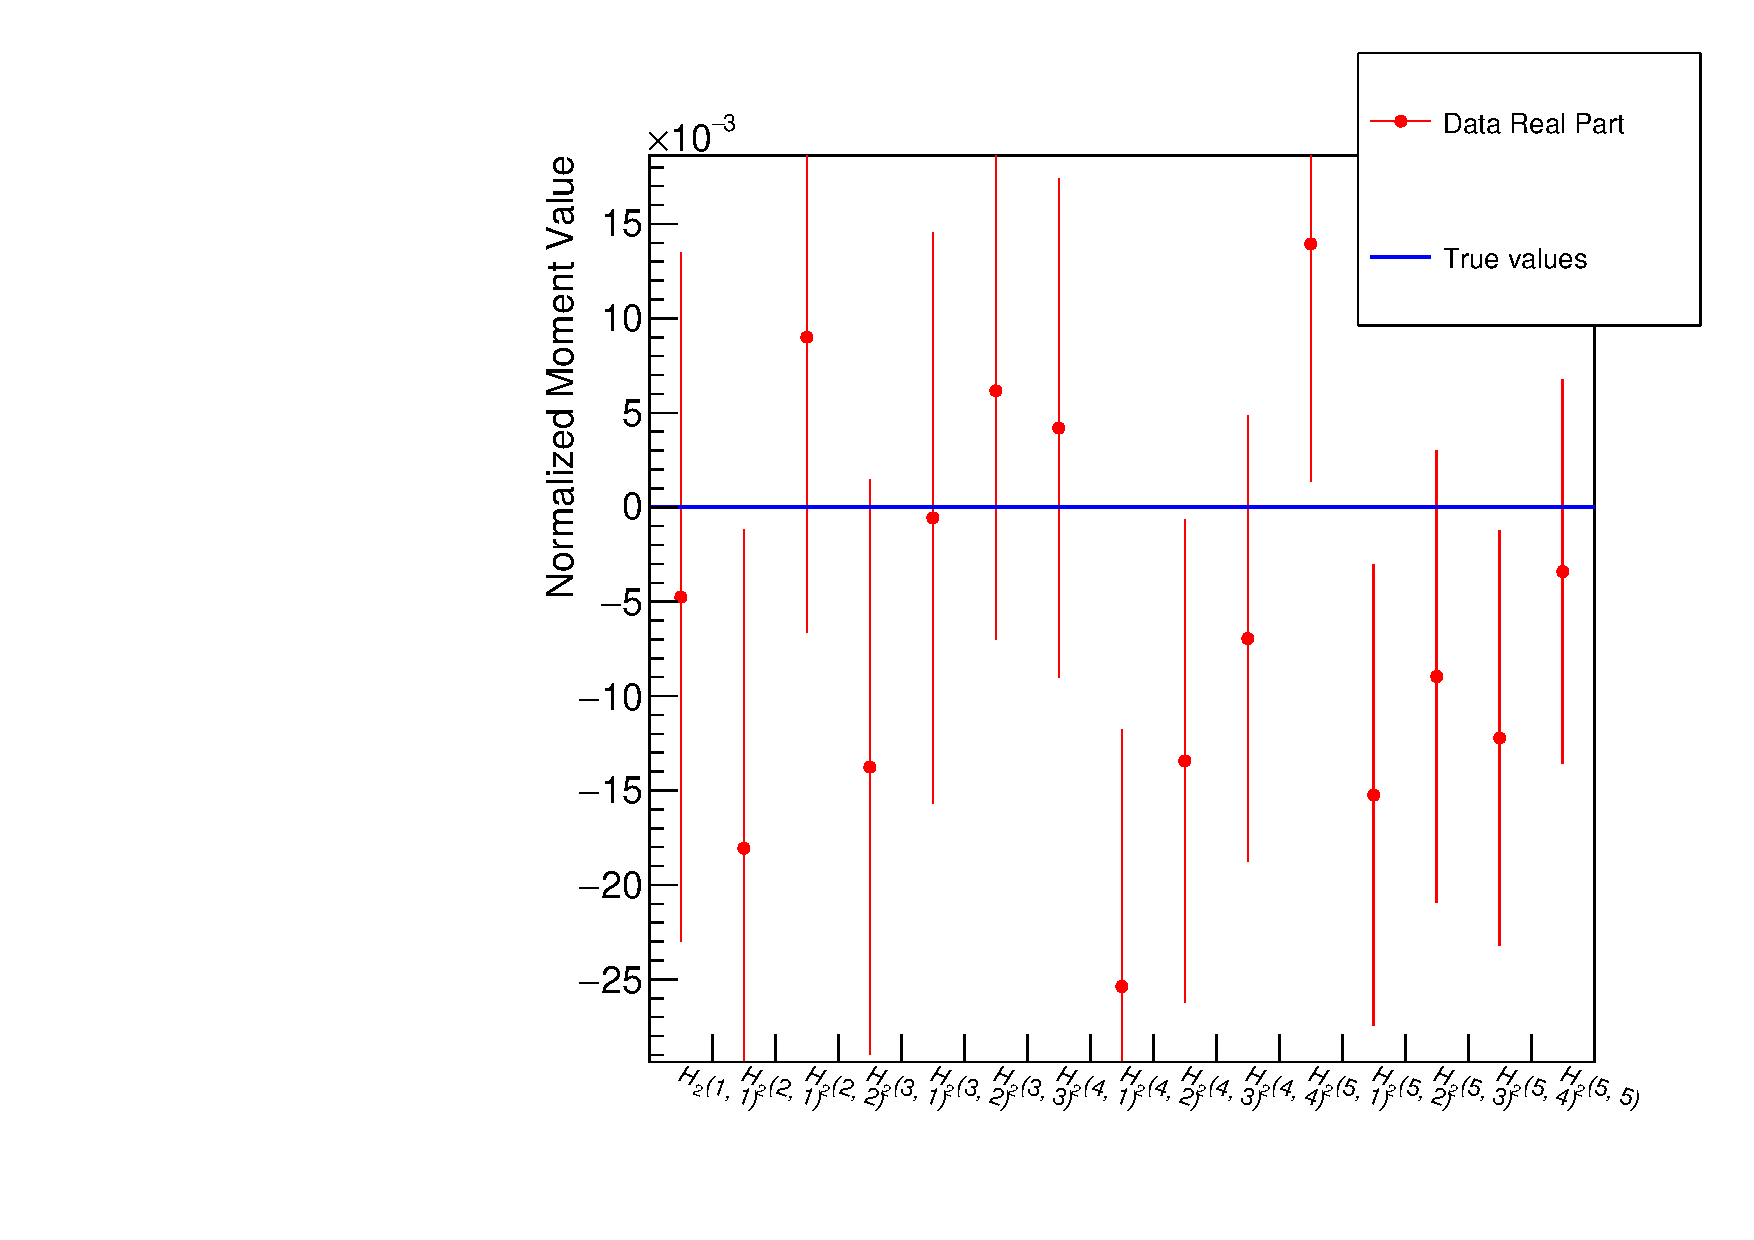
\includegraphics[width=0.5\textwidth]{photoprod_weighted/acc_1/hmass_1.50_Compare_H2_Re}%
  }%
  \subfloat[][]{%
    \label{fig:photoprod_study_weighted_comparison_H2_im}%
    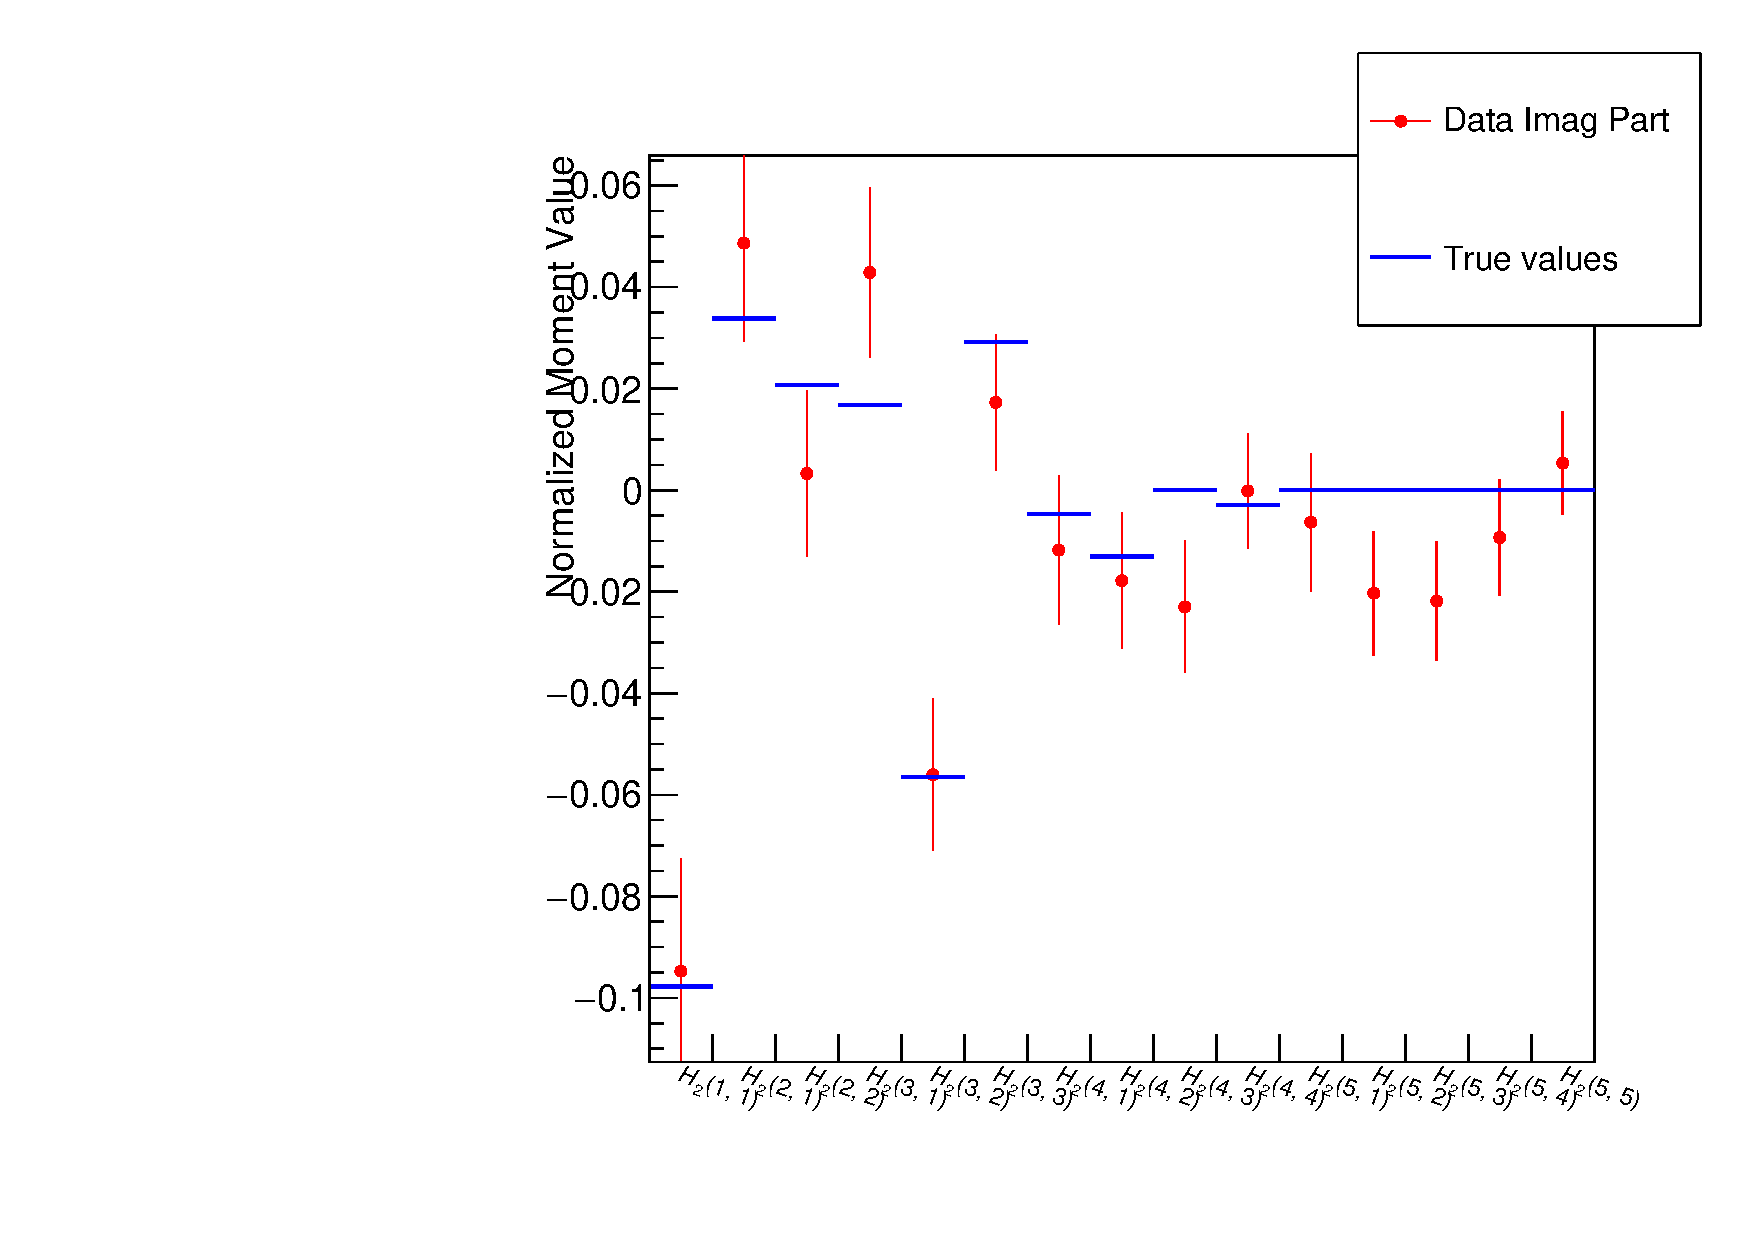
\includegraphics[width=0.5\textwidth]{photoprod_weighted/acc_1/hmass_1.50_Compare_H2_Im}%
  }%
  \\%
  \subfloat[][]{%
    \label{fig:photoprod_study_weighted_residual_H2_re}%
    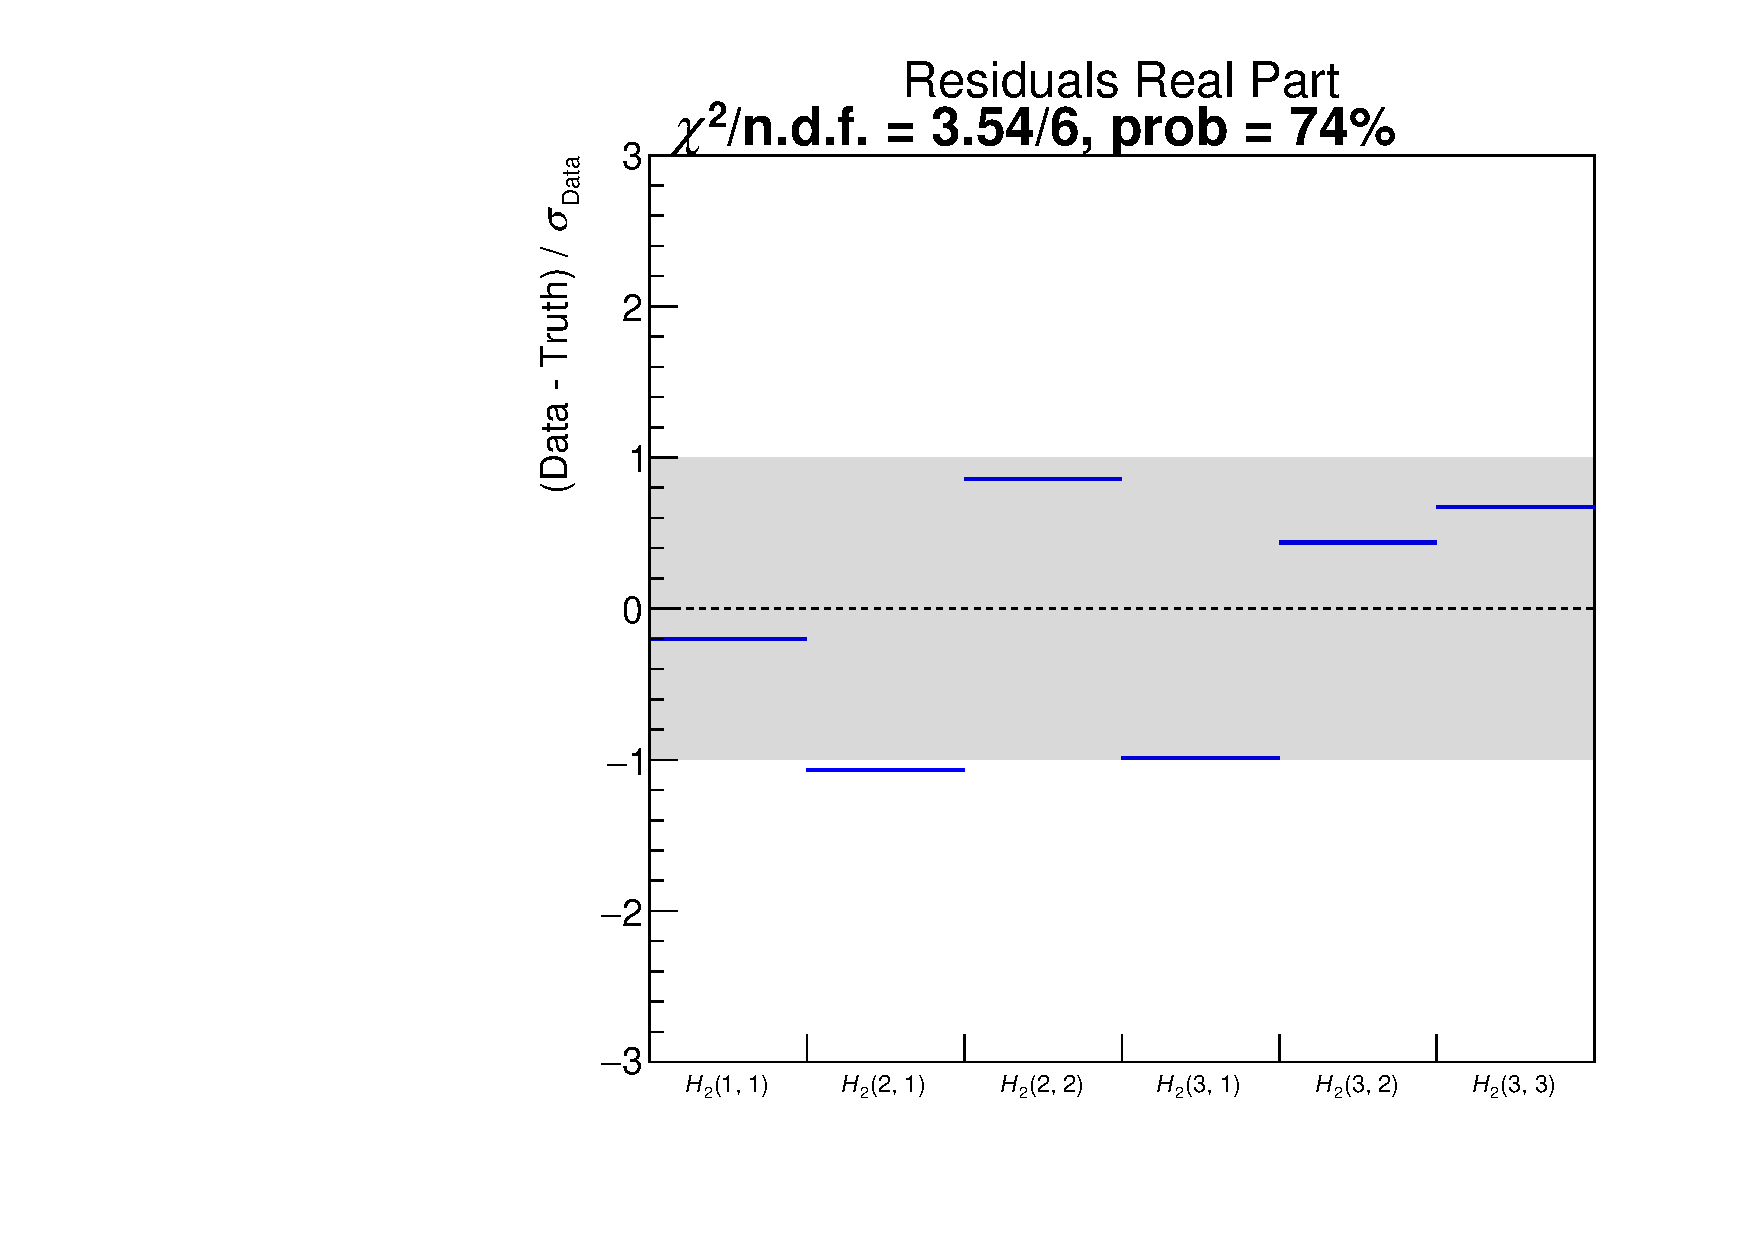
\includegraphics[width=0.5\textwidth]{photoprod_weighted/acc_1/hmass_1.50_Residuals_H2_Re}%
  }%
  \subfloat[][]{%
    \label{fig:photoprod_study_weighted_residual_H2_im}%
    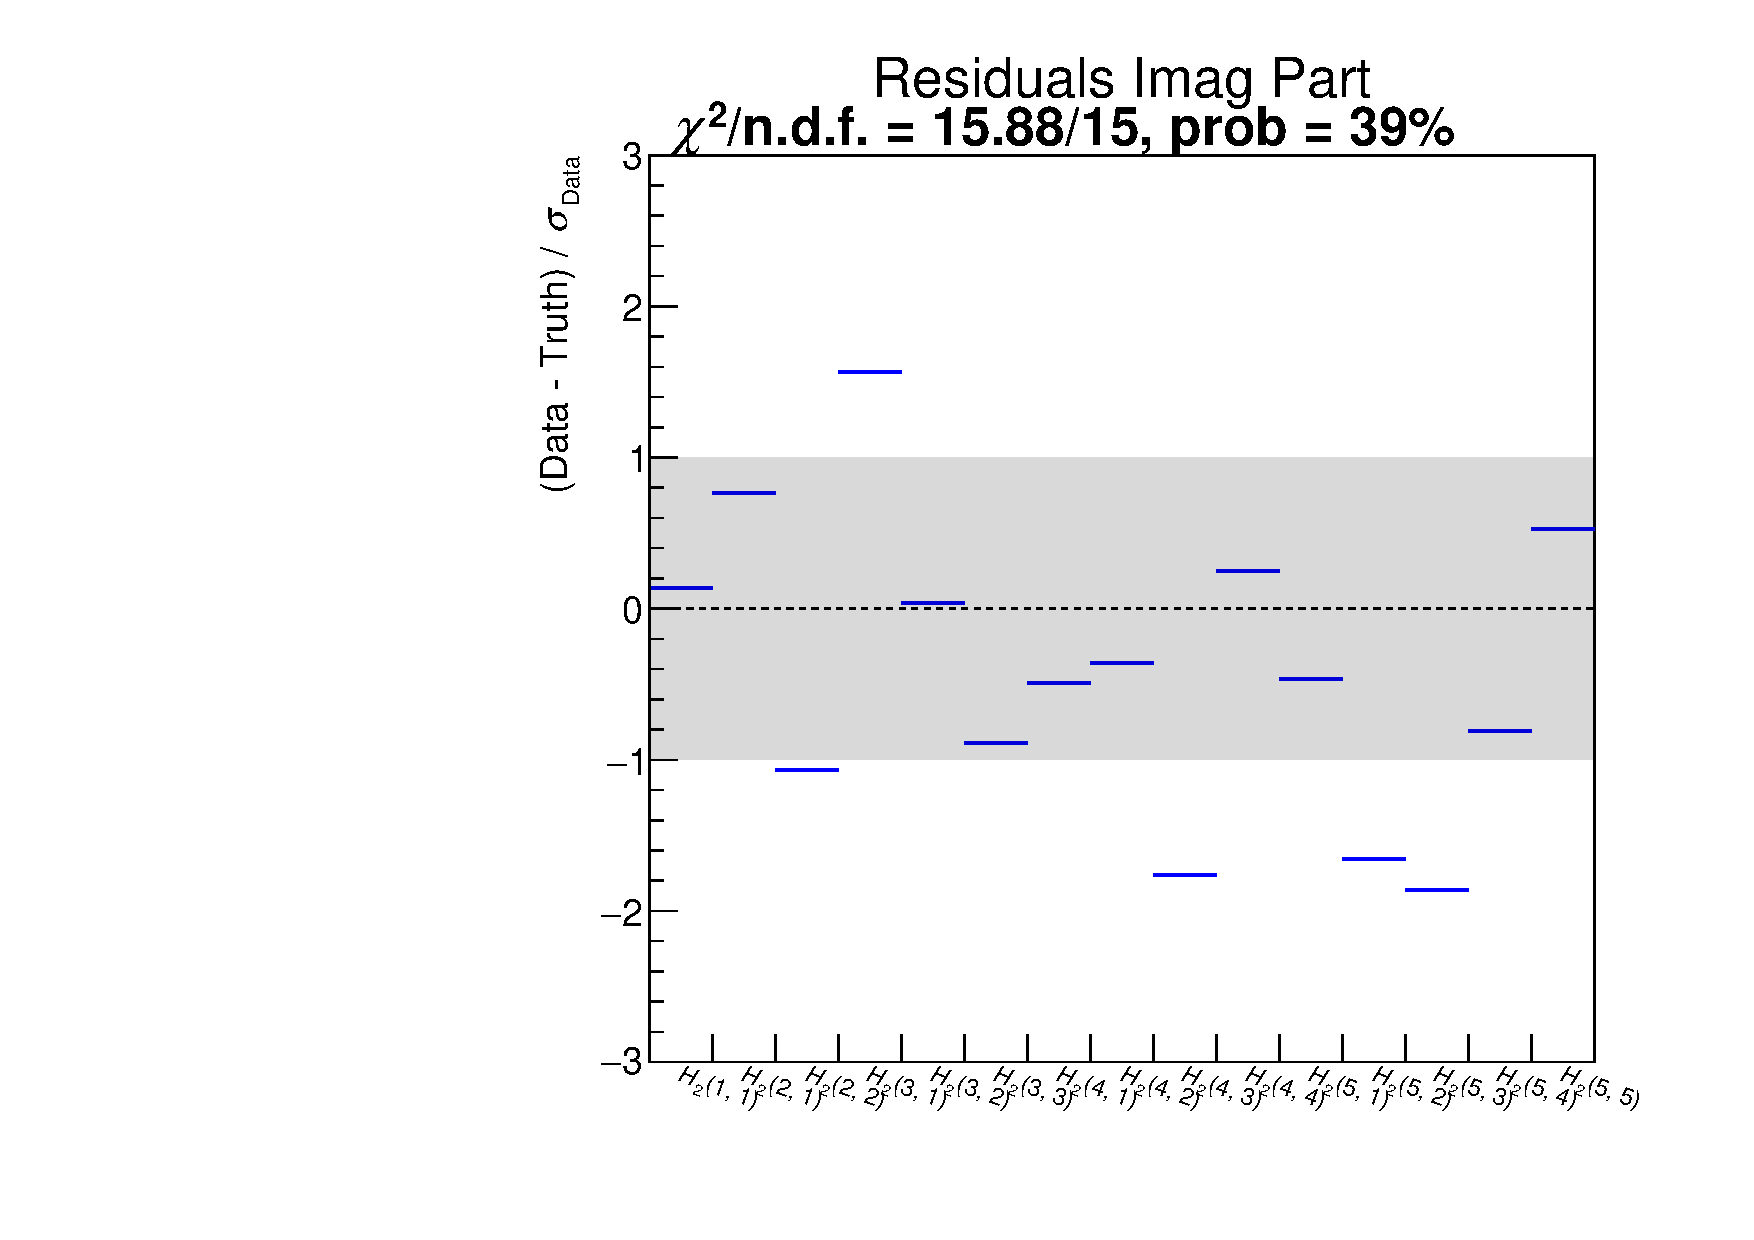
\includegraphics[width=0.5\textwidth]{photoprod_weighted/acc_1/hmass_1.50_Residuals_H2_Im}%
  }%
  \caption{Same as \cref{fig:photoprod_study_weighted_output_H0} but
  for $H_2(L, M)$.}%
  \label{fig:photoprod_study_weighted_output_H2}%
\end{figure}


\clearpage
\subsection{Combining data samples and taking into account time dependence}%
\label{sec:photoprod:comb_data}

Up to now, we assumed that the experimental data used to
estimate~$\vect{H}_\text{meas}$ were taken using the same experimental
conditions.  However, in practice one often has several data samples
that were taken with different experimental conditions, which one
wants to combine.  This means that in general the photon-beam
polarization~$P_\gamma$, the detection efficiency $\eta(\Omega,
\Phi)$, and consequently also the acceptance integral
matrix~$\mat{I}^\text{acc}$ are functions of time.

Given $N_\text{sample}$~data samples indexed by~$j$, each of which
taken using constant experimental conditions represented
by~$\prescript{(j)}{}{P_\gamma}$ and $\prescript{(j)}{}{\eta}(\Omega,
\Phi)$, we calculate the
set~$\Set[1]{\prescript{(j)}{}{\vphantom{\vect{H}}}\hat{\vect{H}}_\text{meas}}$
and the corresponding set of covariance matrices for all data samples
using
\cref{eq:photoprod_moments_meas_estimate_weighted,eq:photoprod_sample_cov_hermit_meas,eq:photoprod_sample_cov_pseudo_meas}.
For each data sample, we also generate an accepted phase-space Monte
Carlo data sample using $\prescript{(j)}{}{\eta}(\Omega, \Phi)$.
Based on these Monte Carlo data, we
calculate~$\prescript{(j)}{}{\mat{I}}^\text{acc}$ using
\cref{eq:photoprod_integral_matrix_mc_weighted}.  Finally, we calculate the
estimates for the physical moments for each data sample using
\cref{eq:diffraction_phys_moments}, \ie
\begin{equation}
  \prescript{(j)}{}{\vphantom{\vect{H}}}\hat{\vect{H}}
  = \rBrk[1]{\prescript{(j)}{}{\mat{I}}^\text{acc}}^{-1}\, \prescript{(j)}{}{\vphantom{\vect{H}}}\hat{\vect{H}}_\text{meas}.
\end{equation}
Note that since the data samples are statistically independent and we
corrected for the different experimental conditions, the set
$\Set[1]{\prescript{(j)}{}{\vphantom{\vect{H}}}\hat{\vect{H}}}$ of
estimates for the physical moments from the various data samples
should be statistically consistent.  Consequently, the values of the
physical moments can be combined using the weighted
average:\footnote{%
This is a straight-forward generalization of the weighted average for
a scalar quantity, which for a data sample $\rbrk{x_1, x_2, \ldots,
x_N}$ of independent measurements~$x_j$ is given by
\begin{equation}
  \mean{x}
  = \frac{\sum_{j = 1}^N w_j\, x_j}{\sum_{j = 1}^N w_j}
  \quad\text{with}\quad
  w_j = \frac{1}{\prescript{(j)}{}{\sigma}_x^2} = \frac{1}{\prescript{(j)}{}{\var{x}}}
  \quad\text{and}\quad
  \var{\mean{x}} = \frac{1}{\sum_{j = 1}^N w_j}.
\end{equation}}
\begin{equation}
  \label{eq:photoprod_datasets_weighted_average}
  \mean{\underaccent{\bar}{\hat{\vect{H}}}}
  = \dUnderbrace{\sBrk[4]{\sum_{j = 1}^{N_\text{sample}} \prescript{(j)}{}{\underaccent{\bar}{\mat{W}}}}^{-1}}{= \hat{\underaccent{\bar}{\covMatSym}}_{\mean{\underaccent{\bar}{\hat{\vect{H}}}}}}
  \sBrk[4]{\sum_{j = 1}^{N_\text{sample}} \prescript{(j)}{}{\underaccent{\bar}{\mat{W}}}\,
  \prescript{(j)}{}{\vphantom{\vect{H}}}\underaccent{\bar}{\hat{\vect{H}}}},
  \quad\text{where}\quad
  \prescript{(j)}{}{\underaccent{\bar}{\mat{W}}}
  = \rBrk[1]{\hat{\underaccent{\bar}{\covMatSym}}_{\!\hat{\vect{H}}}}^{-1}
\end{equation}
is the weight matrix, which is also called precision matrix.  The
statistical consistency of the moment values across the data samples
should be verified by calculating the $P$-value of the
$\chi^2$~statistic of the weighted average.  The $\chi^2$~statistic
for \cref{eq:photoprod_datasets_weighted_average} is
\begin{equation}
  \chi^2
  = \sum_{j = 1}^{N_\text{sample}}
  \sBrk[2]{\prescript{(j)}{}{\vphantom{\vect{H}}}\underaccent{\bar}{\hat{\vect{H}}} - \mean{\underaccent{\bar}{\hat{\vect{H}}}}}^T
  \prescript{(j)}{}{\underaccent{\bar}{\mat{W}}}
  \sBrk[2]{\prescript{(j)}{}{\vphantom{\vect{H}}}\underaccent{\bar}{\hat{\vect{H}}} - \mean{\underaccent{\bar}{\hat{\vect{H}}}}}
\end{equation}
\todo{What is the NDF for weighted events?}


\todo{Discuss separation of reflectivities}

\todo{Add $\eta \pi^0$ example}
